\documentclass[11pt,a4paper]{article}

\usepackage[T1]{fontenc}
\usepackage[utf8]{inputenc}
\usepackage{lmodern}
\usepackage[margin=2.5cm]{geometry}
\usepackage{amsmath,amssymb}
\usepackage{booktabs}
\usepackage{graphicx}
\usepackage{caption}
\usepackage{float}
\usepackage{array}
\newcolumntype{L}[1]{>{\raggedright\arraybackslash}p{#1}}
\newcolumntype{R}[1]{>{\raggedleft\arraybackslash}p{#1}}
\usepackage[nobottomtitles*]{titlesec}
\usepackage{needspace}
\usepackage{placeins}
\usepackage{fancyhdr}
\usepackage{microtype}
\usepackage[hidelinks]{hyperref}
\hypersetup{pdftitle={Scalable Data Loading and Preprocessing with tf.data and TFRecord}, pdfauthor={Xaysomvang (Tom) Thammavong}}

\graphicspath{{../figures/}{../../docs/images/}}

\titleformat{\section}{\large\bfseries}{\thesection}{0.8em}{}
\titleformat{\subsection}{\normalsize\bfseries}{\thesubsection}{0.8em}{}
\titleformat{\paragraph}[runin]{\normalfont\normalsize\bfseries}{}{0em}{}
\titlespacing*{\paragraph}{0pt}{0.9ex plus 0.3ex}{0.7em}
\renewcommand{\bottomtitlespace}{0.15\textheight}
\setlength{\parindent}{0pt}
\widowpenalty=10000
\clubpenalty=10000
% floats: let a figure share a page with text instead of sitting alone on a nearly empty page
\renewcommand{\topfraction}{0.9}
\renewcommand{\bottomfraction}{0.8}
\renewcommand{\textfraction}{0.1}
\renewcommand{\floatpagefraction}{0.8}
\setcounter{topnumber}{3}
\setcounter{totalnumber}{4}
\makeatletter
\setlength{\@fptop}{0pt}
\setlength{\@fpsep}{10pt plus 1fil}
\setlength{\@fpbot}{0pt plus 1fil}
\makeatother
\setlength{\emergencystretch}{2em}
\setlength{\parskip}{0.6em}
\renewcommand{\arraystretch}{1.12}
\captionsetup{font=small,labelfont=bf,labelsep=period}

\pagestyle{fancy}
\fancyhf{}
\renewcommand{\headrulewidth}{0pt}
\fancyfoot[C]{\thepage}

% Generated by make_tables.py. Do not edit.
\newcommand{\metric}[2]{\csname m:#1:#2\endcsname}
\expandafter\newcommand\csname m:A:n_train_rows\endcsname{12,384}
\expandafter\newcommand\csname m:A:pipeline_max_abs_diff_inputs\endcsname{$2.9\times 10^{-6}$}
\expandafter\newcommand\csname m:A:pipeline_max_abs_diff_targets\endcsname{$2.4\times 10^{-7}$}
\expandafter\newcommand\csname m:A:strict_serial_examples_per_s\endcsname{13,412}
\expandafter\newcommand\csname m:A:strict_book_examples_per_s\endcsname{20,606}
\expandafter\newcommand\csname m:A:default_serial_examples_per_s\endcsname{21,484}
\expandafter\newcommand\csname m:A:default_book_examples_per_s\endcsname{19,168}
\expandafter\newcommand\csname m:A:numpy_examples_per_s\endcsname{354,718}
\expandafter\newcommand\csname m:A:numpy_resident_mb\endcsname{1.49}
\expandafter\newcommand\csname m:A:prefetch_speedup_at_slowest_step\endcsname{1.29}
\expandafter\newcommand\csname m:A:slowest_step_ms\endcsname{4}
\expandafter\newcommand\csname m:A:shuffle_spearman_no_shuffle\endcsname{1.0000}
\expandafter\newcommand\csname m:A:shuffle_spearman_buffer_max\endcsname{0.0608}
\expandafter\newcommand\csname m:A:shuffle_buffer_max\endcsname{10,000}
\expandafter\newcommand\csname p:A:batch_size\endcsname{32}
\expandafter\newcommand\csname p:A:repeats\endcsname{5}
\expandafter\newcommand\csname p:A:step_ms_values\endcsname{[0.0, 4.0]}
\expandafter\newcommand\csname p:A:buffer_sizes\endcsname{[100, 1000, 10000]}
\expandafter\newcommand\csname p:A:n_csv_shards\endcsname{20}
\expandafter\newcommand\csname p:A:n_readers\endcsname{5}
\expandafter\newcommand\csname m:B:csv_bytes\endcsname{856,778}
\expandafter\newcommand\csname m:B:csv_gz_bytes\endcsname{287,248}
\expandafter\newcommand\csname m:B:tfrecord_bytes\endcsname{3,576,363}
\expandafter\newcommand\csname m:B:tfrecord_gz_bytes\endcsname{483,662}
\expandafter\newcommand\csname m:B:tfrecord_over_csv\endcsname{4.17}
\expandafter\newcommand\csname m:B:tfrecord_gz_over_csv\endcsname{0.5645}
\expandafter\newcommand\csname m:B:csv_examples_per_s\endcsname{16,602}
\expandafter\newcommand\csname m:B:tfrecord_single_examples_per_s\endcsname{17,964}
\expandafter\newcommand\csname m:B:tfrecord_batch_examples_per_s\endcsname{60,155}
\expandafter\newcommand\csname m:B:tfrecord_gz_batch_examples_per_s\endcsname{62,195}
\expandafter\newcommand\csname m:B:csv_tfrecord_max_abs_diff\endcsname{0}
\expandafter\newcommand\csname m:B:csv_tfrecord_category_equal\endcsname{1}
\expandafter\newcommand\csname m:B:wire_formula_matches_all\endcsname{1}
\expandafter\newcommand\csname m:B:wire_file_bytes_exact\endcsname{1}
\expandafter\newcommand\csname m:B:corruption_all_detected\endcsname{1}
\expandafter\newcommand\csname m:B:missing_feature_default_ok\endcsname{1}
\expandafter\newcommand\csname m:B:scale_rows_max\endcsname{1,238,400}
\expandafter\newcommand\csname m:B:scale_stream_growth_mb_max\endcsname{30.71}
\expandafter\newcommand\csname m:B:scale_pandas_growth_mb_max\endcsname{182}
\expandafter\newcommand\csname m:B:scale_stream_examples_per_s_max\endcsname{60,434}
\expandafter\newcommand\csname p:B:batch_size\endcsname{32}
\expandafter\newcommand\csname p:B:repeats\endcsname{5}
\expandafter\newcommand\csname p:B:scale_copies\endcsname{[1, 10, 100]}
\expandafter\newcommand\csname m:C:n_feature_sets\endcsname{9}
\expandafter\newcommand\csname m:C:n_seeds\endcsname{5}
\expandafter\newcommand\csname m:C:best_feature_set_valid_rmse\endcsname{52,002}
\expandafter\newcommand\csname m:C:best_feature_set_test_rmse\endcsname{50,668}
\expandafter\newcommand\csname m:C:layer_check_max_abs_diff\endcsname{$2.9\times 10^{-6}$}
\expandafter\newcommand\csname m:C:hash_cells\endcsname{400}
\expandafter\newcommand\csname m:C:hash_buckets\endcsname{1,000}
\expandafter\newcommand\csname m:C:hash_cells_with_training_rows\endcsname{133}
\expandafter\newcommand\csname m:C:hash_distinct_buckets_all_cells\endcsname{335}
\expandafter\newcommand\csname m:C:hash_expected_distinct_buckets_all_cells\endcsname{330}
\expandafter\newcommand\csname m:C:hash_distinct_buckets_occupied_cells\endcsname{130}
\expandafter\newcommand\csname m:C:hash_occupied_cells_sharing_a_bucket\endcsname{6}
\expandafter\newcommand\csname m:C:hash_training_rows_in_shared_buckets\endcsname{94}
\expandafter\newcommand\csname m:C:hash_training_rows_in_shared_buckets_pct\endcsname{0.7590}
\expandafter\newcommand\csname m:C:linear_baseline_valid_rmse\endcsname{68,856}
\expandafter\newcommand\csname m:C:linear_best_valid_rmse\endcsname{63,211}
\expandafter\newcommand\csname m:C:linear_n_significant_gains\endcsname{6}
\expandafter\newcommand\csname m:C:mlp_baseline_valid_rmse\endcsname{52,616}
\expandafter\newcommand\csname m:C:mlp_best_valid_rmse\endcsname{52,002}
\expandafter\newcommand\csname m:C:mlp_n_significant_gains\endcsname{1}
\expandafter\newcommand\csname p:C:feature_sets\endcsname{['numeric only', '+ ocean one-hot', '+ ocean embedding', '+ income buckets', '+ age x ocean', '+ grid one-hot (400)', '+ grid embedding (400)', '+ hashed grid (1000)', 'all features']}
\expandafter\newcommand\csname p:C:n_seeds\endcsname{5}
\expandafter\newcommand\csname p:C:heads\endcsname{\{'linear': \{'hidden': [], 'learning\_rate': 0.005, 'epochs': 150, 'patience': 15\}, 'mlp': \{'hidden': [64, 64], 'learning\_rate': 0.002, 'epochs': 100, 'patience': 10\}\}}
\expandafter\newcommand\csname p:C:select_head\endcsname{mlp}
\expandafter\newcommand\csname p:C:best_feature_set\endcsname{+ hashed grid (1000)}
\expandafter\newcommand\csname p:C:batch_size\endcsname{128}
\expandafter\newcommand\csname p:C:compression\endcsname{GZIP}
\expandafter\newcommand\csname m:D:tfds_source_is_mirror\endcsname{1}
\expandafter\newcommand\csname m:D:train_batches\endcsname{1,875}
\expandafter\newcommand\csname m:D:test_batches\endcsname{313}
\expandafter\newcommand\csname m:D:n_train_images\endcsname{60,000}
\expandafter\newcommand\csname m:D:raw_bytes_per_image\endcsname{838}
\expandafter\newcommand\csname m:D:all_encodings_lossless\endcsname{1}
\expandafter\newcommand\csname m:D:tfds_load_test_accuracy\endcsname{0.9757}
\expandafter\newcommand\csname m:D:tfrecord_test_accuracy\endcsname{0.9764}
\expandafter\newcommand\csname p:D:source\endcsname{mirror}
\expandafter\newcommand\csname p:D:epochs\endcsname{5}
\expandafter\newcommand\csname p:D:n_seeds\endcsname{3}
\expandafter\newcommand\csname p:D:n_shards\endcsname{10}
\expandafter\newcommand\csname p:D:element_spec\endcsname{([None, 28, 28, 1], 'uint8')}
\expandafter\newcommand\csname m:E:test_rmse\endcsname{50,751}
\expandafter\newcommand\csname m:E:test_mae\endcsname{34,573}
\expandafter\newcommand\csname m:E:test_r2\endcsname{0.8024}
\expandafter\newcommand\csname m:E:baseline_linear_test_rmse\endcsname{67,368}
\expandafter\newcommand\csname m:E:skew_max_abs_usd\endcsname{0}
\expandafter\newcommand\csname m:E:unknown_category_ok\endcsname{1}
\expandafter\newcommand\csname m:E:missing_value_ok\endcsname{1}
\expandafter\newcommand\csname m:E:valid_rmse\endcsname{52,495}
\expandafter\newcommand\csname m:E:valid_r2\endcsname{0.7954}
\expandafter\newcommand\csname m:E:baseline_mean_test_rmse\endcsname{114,164}
\expandafter\newcommand\csname m:E:roundtrip_max_abs_usd\endcsname{0}
\expandafter\newcommand\csname m:E:epochs_run\endcsname{55}
\expandafter\newcommand\csname m:E:best_epoch\endcsname{45}
\expandafter\newcommand\csname m:E:train_seconds\endcsname{17.72}
\expandafter\newcommand\csname m:E:n_params\endcsname{13,697}
\expandafter\newcommand\csname m:E:rows_with_missing_value\endcsname{49}
\expandafter\newcommand\csname m:E:rows_outside_training_range\endcsname{3}
\expandafter\newcommand\csname p:E:feature_set\endcsname{+ hashed grid (1000)}
\expandafter\newcommand\csname p:E:hidden\endcsname{[64, 64]}
\expandafter\newcommand\csname p:E:compression\endcsname{GZIP}
\expandafter\newcommand\csname p:E:seed\endcsname{42}
\newcommand{\val}[1]{\csname v:#1\endcsname}
\expandafter\newcommand\csname v:abl:default:0:1\endcsname{21,484}
\expandafter\newcommand\csname v:abl:default:0:2\endcsname{19,019}
\expandafter\newcommand\csname v:abl:default:0:3\endcsname{19,189}
\expandafter\newcommand\csname v:abl:default:0:4\endcsname{25,885}
\expandafter\newcommand\csname v:abl:default:0:5\endcsname{19,168}
\expandafter\newcommand\csname v:abl:default:0:6\endcsname{15,104}
\expandafter\newcommand\csname v:ablr:default:0:2:1\endcsname{0.89}
\expandafter\newcommand\csname v:ablr:default:0:3:2\endcsname{1.01}
\expandafter\newcommand\csname v:ablr:default:0:4:3\endcsname{1.35}
\expandafter\newcommand\csname v:ablr:default:0:5:4\endcsname{0.74}
\expandafter\newcommand\csname v:ablr:default:0:6:5\endcsname{0.79}
\expandafter\newcommand\csname v:ablr:default:0:5:1\endcsname{0.89}
\expandafter\newcommand\csname v:ablr:default:0:5:6\endcsname{1.27}
\expandafter\newcommand\csname v:abl:default:4:1\endcsname{6,822}
\expandafter\newcommand\csname v:abl:default:4:2\endcsname{6,851}
\expandafter\newcommand\csname v:abl:default:4:3\endcsname{6,711}
\expandafter\newcommand\csname v:abl:default:4:4\endcsname{6,686}
\expandafter\newcommand\csname v:abl:default:4:5\endcsname{6,692}
\expandafter\newcommand\csname v:abl:default:4:6\endcsname{6,612}
\expandafter\newcommand\csname v:ablr:default:4:2:1\endcsname{1.00}
\expandafter\newcommand\csname v:ablr:default:4:3:2\endcsname{0.98}
\expandafter\newcommand\csname v:ablr:default:4:4:3\endcsname{1.00}
\expandafter\newcommand\csname v:ablr:default:4:5:4\endcsname{1.00}
\expandafter\newcommand\csname v:ablr:default:4:6:5\endcsname{0.99}
\expandafter\newcommand\csname v:ablr:default:4:5:1\endcsname{0.98}
\expandafter\newcommand\csname v:ablr:default:4:5:6\endcsname{1.01}
\expandafter\newcommand\csname v:abl:strict:0:1\endcsname{13,412}
\expandafter\newcommand\csname v:abl:strict:0:2\endcsname{15,632}
\expandafter\newcommand\csname v:abl:strict:0:3\endcsname{16,039}
\expandafter\newcommand\csname v:abl:strict:0:4\endcsname{18,935}
\expandafter\newcommand\csname v:abl:strict:0:5\endcsname{20,606}
\expandafter\newcommand\csname v:abl:strict:0:6\endcsname{15,525}
\expandafter\newcommand\csname v:ablr:strict:0:2:1\endcsname{1.17}
\expandafter\newcommand\csname v:ablr:strict:0:3:2\endcsname{1.03}
\expandafter\newcommand\csname v:ablr:strict:0:4:3\endcsname{1.18}
\expandafter\newcommand\csname v:ablr:strict:0:5:4\endcsname{1.09}
\expandafter\newcommand\csname v:ablr:strict:0:6:5\endcsname{0.75}
\expandafter\newcommand\csname v:ablr:strict:0:5:1\endcsname{1.54}
\expandafter\newcommand\csname v:ablr:strict:0:5:6\endcsname{1.33}
\expandafter\newcommand\csname v:abl:strict:4:1\endcsname{4,826}
\expandafter\newcommand\csname v:abl:strict:4:2\endcsname{4,792}
\expandafter\newcommand\csname v:abl:strict:4:3\endcsname{4,969}
\expandafter\newcommand\csname v:abl:strict:4:4\endcsname{5,275}
\expandafter\newcommand\csname v:abl:strict:4:5\endcsname{6,794}
\expandafter\newcommand\csname v:abl:strict:4:6\endcsname{6,646}
\expandafter\newcommand\csname v:ablr:strict:4:2:1\endcsname{0.99}
\expandafter\newcommand\csname v:ablr:strict:4:3:2\endcsname{1.04}
\expandafter\newcommand\csname v:ablr:strict:4:4:3\endcsname{1.06}
\expandafter\newcommand\csname v:ablr:strict:4:5:4\endcsname{1.29}
\expandafter\newcommand\csname v:ablr:strict:4:6:5\endcsname{0.98}
\expandafter\newcommand\csname v:ablr:strict:4:5:1\endcsname{1.41}
\expandafter\newcommand\csname v:ablr:strict:4:5:6\endcsname{1.02}
\expandafter\newcommand\csname v:gain:strict:0:min\endcsname{1.03}
\expandafter\newcommand\csname v:gain:strict:0:max\endcsname{1.18}
\expandafter\newcommand\csname v:abl:strict:4:min14\endcsname{4,792}
\expandafter\newcommand\csname v:abl:strict:4:max14\endcsname{5,275}
\expandafter\newcommand\csname v:abl:default:4:spread\endcsname{3.6}
\expandafter\newcommand\csname v:abl:default:0:min\endcsname{15,104}
\expandafter\newcommand\csname v:abl:default:0:max\endcsname{25,885}
\expandafter\newcommand\csname v:abl:0:max\endcsname{25,885}
\expandafter\newcommand\csname v:numpy:0\endcsname{354,718}
\expandafter\newcommand\csname v:numpy:4\endcsname{7,530}
\expandafter\newcommand\csname v:numpy:over:book:0\endcsname{17.2}
\expandafter\newcommand\csname v:numpy:book:share:4\endcsname{90}
\expandafter\newcommand\csname v:bound:4\endcsname{8,000}
\expandafter\newcommand\csname v:sweep:over:min\endcsname{0.66}
\expandafter\newcommand\csname v:sweep:over:max\endcsname{0.76}
\expandafter\newcommand\csname v:sweep:serial:over:min\endcsname{0.38}
\expandafter\newcommand\csname v:sweep:serial:over:max\endcsname{0.59}
\expandafter\newcommand\csname v:eq:missing\endcsname{124}
\expandafter\newcommand\csname v:eq:rows\endcsname{12,384}
\expandafter\newcommand\csname v:sweep:batches\endcsname{387}
\expandafter\newcommand\csname v:shuf:no-shuffling:rho\endcsname{1.000}
\expandafter\newcommand\csname v:shuf:no-shuffling:div\endcsname{0.006}
\expandafter\newcommand\csname v:shuf:random-file-order-only:rho\endcsname{$-$0.011}
\expandafter\newcommand\csname v:shuf:random-file-order-only:div\endcsname{0.058}
\expandafter\newcommand\csname v:shuf:interleave-5-files:rho\endcsname{0.005}
\expandafter\newcommand\csname v:shuf:interleave-5-files:div\endcsname{0.920}
\expandafter\newcommand\csname v:shuf:buffer-100:rho\endcsname{1.000}
\expandafter\newcommand\csname v:shuf:buffer-100:div\endcsname{0.033}
\expandafter\newcommand\csname v:shuf:buffer-100:pred\endcsname{1.000}
\expandafter\newcommand\csname v:shuf:buffer-1000:rho\endcsname{0.965}
\expandafter\newcommand\csname v:shuf:buffer-1000:div\endcsname{0.267}
\expandafter\newcommand\csname v:shuf:buffer-1000:pred\endcsname{0.963}
\expandafter\newcommand\csname v:shuf:buffer-10000:rho\endcsname{0.061}
\expandafter\newcommand\csname v:shuf:buffer-10000:div\endcsname{0.974}
\expandafter\newcommand\csname v:shuf:interleave-5-buffer-100:rho\endcsname{0.005}
\expandafter\newcommand\csname v:shuf:interleave-5-buffer-100:div\endcsname{0.916}
\expandafter\newcommand\csname v:shuf:interleave-5-buffer-1000:rho\endcsname{0.006}
\expandafter\newcommand\csname v:shuf:interleave-5-buffer-1000:div\endcsname{0.943}
\expandafter\newcommand\csname v:shuf:interleave-5-buffer-10000:rho\endcsname{$-$0.010}
\expandafter\newcommand\csname v:shuf:interleave-5-buffer-10000:div\endcsname{0.987}
\expandafter\newcommand\csname v:shuf:buf10000:frac\endcsname{81}
\expandafter\newcommand\csname v:shuf:npred\endcsname{2}
\expandafter\newcommand\csname v:shuf:maxdev\endcsname{0.002}
\expandafter\newcommand\csname v:c:linear:numeric-only:valid\endcsname{69,626}
\expandafter\newcommand\csname v:c:linear:numeric-only:test\endcsname{68,473}
\expandafter\newcommand\csname v:c:linear:numeric-only:r2\endcsname{0.640}
\expandafter\newcommand\csname v:c:linear:numeric-only:params\endcsname{9}
\expandafter\newcommand\csname v:c:linear:numeric-only:features\endcsname{8}
\expandafter\newcommand\csname v:c:linear:numeric-only:diff\endcsname{770}
\expandafter\newcommand\csname v:c:linear:numeric-only:difflo\endcsname{746}
\expandafter\newcommand\csname v:c:linear:numeric-only:diffhi\endcsname{793}
\expandafter\newcommand\csname v:c:linear:numeric-only:pct\endcsname{1.1}
\expandafter\newcommand\csname v:c:linear:ocean-one-hot:valid\endcsname{68,856}
\expandafter\newcommand\csname v:c:linear:ocean-one-hot:test\endcsname{67,490}
\expandafter\newcommand\csname v:c:linear:ocean-one-hot:r2\endcsname{0.651}
\expandafter\newcommand\csname v:c:linear:ocean-one-hot:params\endcsname{15}
\expandafter\newcommand\csname v:c:linear:ocean-one-hot:features\endcsname{14}
\expandafter\newcommand\csname v:c:linear:ocean-embedding:valid\endcsname{68,902}
\expandafter\newcommand\csname v:c:linear:ocean-embedding:test\endcsname{67,462}
\expandafter\newcommand\csname v:c:linear:ocean-embedding:r2\endcsname{0.651}
\expandafter\newcommand\csname v:c:linear:ocean-embedding:params\endcsname{23}
\expandafter\newcommand\csname v:c:linear:ocean-embedding:features\endcsname{10}
\expandafter\newcommand\csname v:c:linear:ocean-embedding:diff\endcsname{46}
\expandafter\newcommand\csname v:c:linear:ocean-embedding:difflo\endcsname{2}
\expandafter\newcommand\csname v:c:linear:ocean-embedding:diffhi\endcsname{89}
\expandafter\newcommand\csname v:c:linear:ocean-embedding:pct\endcsname{0.1}
\expandafter\newcommand\csname v:c:linear:income-buckets:valid\endcsname{67,980}
\expandafter\newcommand\csname v:c:linear:income-buckets:test\endcsname{66,604}
\expandafter\newcommand\csname v:c:linear:income-buckets:r2\endcsname{0.660}
\expandafter\newcommand\csname v:c:linear:income-buckets:params\endcsname{20}
\expandafter\newcommand\csname v:c:linear:income-buckets:features\endcsname{19}
\expandafter\newcommand\csname v:c:linear:income-buckets:diff\endcsname{876}
\expandafter\newcommand\csname v:c:linear:income-buckets:difflo\endcsname{901}
\expandafter\newcommand\csname v:c:linear:income-buckets:diffhi\endcsname{850}
\expandafter\newcommand\csname v:c:linear:income-buckets:pct\endcsname{1.3}
\expandafter\newcommand\csname v:c:linear:age-x-ocean:valid\endcsname{68,580}
\expandafter\newcommand\csname v:c:linear:age-x-ocean:test\endcsname{67,149}
\expandafter\newcommand\csname v:c:linear:age-x-ocean:r2\endcsname{0.654}
\expandafter\newcommand\csname v:c:linear:age-x-ocean:params\endcsname{419}
\expandafter\newcommand\csname v:c:linear:age-x-ocean:features\endcsname{18}
\expandafter\newcommand\csname v:c:linear:age-x-ocean:diff\endcsname{276}
\expandafter\newcommand\csname v:c:linear:age-x-ocean:difflo\endcsname{309}
\expandafter\newcommand\csname v:c:linear:age-x-ocean:diffhi\endcsname{243}
\expandafter\newcommand\csname v:c:linear:age-x-ocean:pct\endcsname{0.4}
\expandafter\newcommand\csname v:c:linear:grid-one-hot-400:valid\endcsname{64,226}
\expandafter\newcommand\csname v:c:linear:grid-one-hot-400:test\endcsname{62,546}
\expandafter\newcommand\csname v:c:linear:grid-one-hot-400:r2\endcsname{0.700}
\expandafter\newcommand\csname v:c:linear:grid-one-hot-400:params\endcsname{415}
\expandafter\newcommand\csname v:c:linear:grid-one-hot-400:features\endcsname{414}
\expandafter\newcommand\csname v:c:linear:grid-one-hot-400:diff\endcsname{4,630}
\expandafter\newcommand\csname v:c:linear:grid-one-hot-400:difflo\endcsname{4,657}
\expandafter\newcommand\csname v:c:linear:grid-one-hot-400:diffhi\endcsname{4,602}
\expandafter\newcommand\csname v:c:linear:grid-one-hot-400:pct\endcsname{6.7}
\expandafter\newcommand\csname v:c:linear:grid-embedding-400:valid\endcsname{64,583}
\expandafter\newcommand\csname v:c:linear:grid-embedding-400:test\endcsname{62,787}
\expandafter\newcommand\csname v:c:linear:grid-embedding-400:r2\endcsname{0.698}
\expandafter\newcommand\csname v:c:linear:grid-embedding-400:params\endcsname{3,223}
\expandafter\newcommand\csname v:c:linear:grid-embedding-400:features\endcsname{22}
\expandafter\newcommand\csname v:c:linear:grid-embedding-400:diff\endcsname{4,273}
\expandafter\newcommand\csname v:c:linear:grid-embedding-400:difflo\endcsname{4,371}
\expandafter\newcommand\csname v:c:linear:grid-embedding-400:diffhi\endcsname{4,174}
\expandafter\newcommand\csname v:c:linear:grid-embedding-400:pct\endcsname{6.2}
\expandafter\newcommand\csname v:c:linear:hashed-grid-1000:valid\endcsname{64,675}
\expandafter\newcommand\csname v:c:linear:hashed-grid-1000:test\endcsname{62,846}
\expandafter\newcommand\csname v:c:linear:hashed-grid-1000:r2\endcsname{0.697}
\expandafter\newcommand\csname v:c:linear:hashed-grid-1000:params\endcsname{8,023}
\expandafter\newcommand\csname v:c:linear:hashed-grid-1000:features\endcsname{22}
\expandafter\newcommand\csname v:c:linear:hashed-grid-1000:diff\endcsname{4,182}
\expandafter\newcommand\csname v:c:linear:hashed-grid-1000:difflo\endcsname{4,352}
\expandafter\newcommand\csname v:c:linear:hashed-grid-1000:diffhi\endcsname{4,011}
\expandafter\newcommand\csname v:c:linear:hashed-grid-1000:pct\endcsname{6.1}
\expandafter\newcommand\csname v:c:linear:all-features:valid\endcsname{63,211}
\expandafter\newcommand\csname v:c:linear:all-features:test\endcsname{61,316}
\expandafter\newcommand\csname v:c:linear:all-features:r2\endcsname{0.712}
\expandafter\newcommand\csname v:c:linear:all-features:params\endcsname{8,432}
\expandafter\newcommand\csname v:c:linear:all-features:features\endcsname{31}
\expandafter\newcommand\csname v:c:linear:all-features:diff\endcsname{5,645}
\expandafter\newcommand\csname v:c:linear:all-features:difflo\endcsname{5,737}
\expandafter\newcommand\csname v:c:linear:all-features:diffhi\endcsname{5,553}
\expandafter\newcommand\csname v:c:linear:all-features:pct\endcsname{8.2}
\expandafter\newcommand\csname v:c:linear:base\endcsname{68,856}
\expandafter\newcommand\csname v:c:linear:base:test\endcsname{67,490}
\expandafter\newcommand\csname v:c:linear:nbetter\endcsname{6}
\expandafter\newcommand\csname v:c:linear:nworse\endcsname{2}
\expandafter\newcommand\csname v:c:linear:ncompared\endcsname{8}
\expandafter\newcommand\csname v:c:linear:best:name\endcsname{all features}
\expandafter\newcommand\csname v:c:linear:best\endcsname{63,211}
\expandafter\newcommand\csname v:c:mlp:numeric-only:valid\endcsname{52,303}
\expandafter\newcommand\csname v:c:mlp:numeric-only:test\endcsname{51,852}
\expandafter\newcommand\csname v:c:mlp:numeric-only:r2\endcsname{0.794}
\expandafter\newcommand\csname v:c:mlp:numeric-only:params\endcsname{4,801}
\expandafter\newcommand\csname v:c:mlp:numeric-only:features\endcsname{8}
\expandafter\newcommand\csname v:c:mlp:numeric-only:diff\endcsname{312}
\expandafter\newcommand\csname v:c:mlp:numeric-only:difflo\endcsname{1,088}
\expandafter\newcommand\csname v:c:mlp:numeric-only:diffhi\endcsname{464}
\expandafter\newcommand\csname v:c:mlp:numeric-only:pct\endcsname{0.6}
\expandafter\newcommand\csname v:c:mlp:ocean-one-hot:valid\endcsname{52,616}
\expandafter\newcommand\csname v:c:mlp:ocean-one-hot:test\endcsname{51,530}
\expandafter\newcommand\csname v:c:mlp:ocean-one-hot:r2\endcsname{0.796}
\expandafter\newcommand\csname v:c:mlp:ocean-one-hot:params\endcsname{5,185}
\expandafter\newcommand\csname v:c:mlp:ocean-one-hot:features\endcsname{14}
\expandafter\newcommand\csname v:c:mlp:ocean-embedding:valid\endcsname{52,180}
\expandafter\newcommand\csname v:c:mlp:ocean-embedding:test\endcsname{51,387}
\expandafter\newcommand\csname v:c:mlp:ocean-embedding:r2\endcsname{0.797}
\expandafter\newcommand\csname v:c:mlp:ocean-embedding:params\endcsname{4,941}
\expandafter\newcommand\csname v:c:mlp:ocean-embedding:features\endcsname{10}
\expandafter\newcommand\csname v:c:mlp:ocean-embedding:diff\endcsname{436}
\expandafter\newcommand\csname v:c:mlp:ocean-embedding:difflo\endcsname{1,159}
\expandafter\newcommand\csname v:c:mlp:ocean-embedding:diffhi\endcsname{287}
\expandafter\newcommand\csname v:c:mlp:ocean-embedding:pct\endcsname{0.8}
\expandafter\newcommand\csname v:c:mlp:income-buckets:valid\endcsname{53,079}
\expandafter\newcommand\csname v:c:mlp:income-buckets:test\endcsname{51,730}
\expandafter\newcommand\csname v:c:mlp:income-buckets:r2\endcsname{0.795}
\expandafter\newcommand\csname v:c:mlp:income-buckets:params\endcsname{5,505}
\expandafter\newcommand\csname v:c:mlp:income-buckets:features\endcsname{19}
\expandafter\newcommand\csname v:c:mlp:income-buckets:diff\endcsname{463}
\expandafter\newcommand\csname v:c:mlp:income-buckets:difflo\endcsname{133}
\expandafter\newcommand\csname v:c:mlp:income-buckets:diffhi\endcsname{1,059}
\expandafter\newcommand\csname v:c:mlp:income-buckets:pct\endcsname{0.9}
\expandafter\newcommand\csname v:c:mlp:age-x-ocean:valid\endcsname{52,706}
\expandafter\newcommand\csname v:c:mlp:age-x-ocean:test\endcsname{51,814}
\expandafter\newcommand\csname v:c:mlp:age-x-ocean:r2\endcsname{0.794}
\expandafter\newcommand\csname v:c:mlp:age-x-ocean:params\endcsname{5,841}
\expandafter\newcommand\csname v:c:mlp:age-x-ocean:features\endcsname{18}
\expandafter\newcommand\csname v:c:mlp:age-x-ocean:diff\endcsname{90}
\expandafter\newcommand\csname v:c:mlp:age-x-ocean:difflo\endcsname{488}
\expandafter\newcommand\csname v:c:mlp:age-x-ocean:diffhi\endcsname{669}
\expandafter\newcommand\csname v:c:mlp:age-x-ocean:pct\endcsname{0.2}
\expandafter\newcommand\csname v:c:mlp:grid-one-hot-400:valid\endcsname{52,759}
\expandafter\newcommand\csname v:c:mlp:grid-one-hot-400:test\endcsname{51,590}
\expandafter\newcommand\csname v:c:mlp:grid-one-hot-400:r2\endcsname{0.796}
\expandafter\newcommand\csname v:c:mlp:grid-one-hot-400:params\endcsname{30,785}
\expandafter\newcommand\csname v:c:mlp:grid-one-hot-400:features\endcsname{414}
\expandafter\newcommand\csname v:c:mlp:grid-one-hot-400:diff\endcsname{143}
\expandafter\newcommand\csname v:c:mlp:grid-one-hot-400:difflo\endcsname{356}
\expandafter\newcommand\csname v:c:mlp:grid-one-hot-400:diffhi\endcsname{642}
\expandafter\newcommand\csname v:c:mlp:grid-one-hot-400:pct\endcsname{0.3}
\expandafter\newcommand\csname v:c:mlp:grid-embedding-400:valid\endcsname{52,230}
\expandafter\newcommand\csname v:c:mlp:grid-embedding-400:test\endcsname{51,065}
\expandafter\newcommand\csname v:c:mlp:grid-embedding-400:r2\endcsname{0.800}
\expandafter\newcommand\csname v:c:mlp:grid-embedding-400:params\endcsname{8,897}
\expandafter\newcommand\csname v:c:mlp:grid-embedding-400:features\endcsname{22}
\expandafter\newcommand\csname v:c:mlp:grid-embedding-400:diff\endcsname{385}
\expandafter\newcommand\csname v:c:mlp:grid-embedding-400:difflo\endcsname{964}
\expandafter\newcommand\csname v:c:mlp:grid-embedding-400:diffhi\endcsname{193}
\expandafter\newcommand\csname v:c:mlp:grid-embedding-400:pct\endcsname{0.7}
\expandafter\newcommand\csname v:c:mlp:hashed-grid-1000:valid\endcsname{52,002}
\expandafter\newcommand\csname v:c:mlp:hashed-grid-1000:test\endcsname{50,668}
\expandafter\newcommand\csname v:c:mlp:hashed-grid-1000:r2\endcsname{0.803}
\expandafter\newcommand\csname v:c:mlp:hashed-grid-1000:params\endcsname{13,697}
\expandafter\newcommand\csname v:c:mlp:hashed-grid-1000:features\endcsname{22}
\expandafter\newcommand\csname v:c:mlp:hashed-grid-1000:diff\endcsname{614}
\expandafter\newcommand\csname v:c:mlp:hashed-grid-1000:difflo\endcsname{1,191}
\expandafter\newcommand\csname v:c:mlp:hashed-grid-1000:diffhi\endcsname{36}
\expandafter\newcommand\csname v:c:mlp:hashed-grid-1000:pct\endcsname{1.2}
\expandafter\newcommand\csname v:c:mlp:all-features:valid\endcsname{52,803}
\expandafter\newcommand\csname v:c:mlp:all-features:test\endcsname{51,606}
\expandafter\newcommand\csname v:c:mlp:all-features:r2\endcsname{0.796}
\expandafter\newcommand\csname v:c:mlp:all-features:params\endcsname{14,673}
\expandafter\newcommand\csname v:c:mlp:all-features:features\endcsname{31}
\expandafter\newcommand\csname v:c:mlp:all-features:diff\endcsname{188}
\expandafter\newcommand\csname v:c:mlp:all-features:difflo\endcsname{586}
\expandafter\newcommand\csname v:c:mlp:all-features:diffhi\endcsname{961}
\expandafter\newcommand\csname v:c:mlp:all-features:pct\endcsname{0.4}
\expandafter\newcommand\csname v:c:mlp:base\endcsname{52,616}
\expandafter\newcommand\csname v:c:mlp:base:test\endcsname{51,530}
\expandafter\newcommand\csname v:c:mlp:nbetter\endcsname{1}
\expandafter\newcommand\csname v:c:mlp:nworse\endcsname{0}
\expandafter\newcommand\csname v:c:mlp:ncompared\endcsname{8}
\expandafter\newcommand\csname v:c:mlp:best:name\endcsname{+ hashed grid (1000)}
\expandafter\newcommand\csname v:c:mlp:best\endcsname{52,002}
\expandafter\newcommand\csname v:c:mlp:over:linear:pct\endcsname{23.6}
\expandafter\newcommand\csname v:hash:shared:cells\endcsname{65}
\expandafter\newcommand\csname v:hash:expected:shared\endcsname{70.2}
\expandafter\newcommand\csname v:hash:expected\endcsname{329.8}
\expandafter\newcommand\csname v:hash:rows:pct\endcsname{0.76}
\expandafter\newcommand\csname v:fmt:batch:over:csv\endcsname{3.6}
\expandafter\newcommand\csname v:fmt:batchgz:over:csv\endcsname{3.7}
\expandafter\newcommand\csname v:fmt:batch:over:single\endcsname{3.3}
\expandafter\newcommand\csname v:fmt:single:over:csv\endcsname{1.08}
\expandafter\newcommand\csname v:fmt:max\endcsname{62,195}
\expandafter\newcommand\csname v:fmt:csvgz:size\endcsname{0.34}
\expandafter\newcommand\csname v:fmt:tfr:size\endcsname{4.17}
\expandafter\newcommand\csname v:fmt:tfrgz:size\endcsname{0.56}
\expandafter\newcommand\csname v:fmt:tfrgz:over:csvgz\endcsname{1.68}
\expandafter\newcommand\csname v:wire:min\endcsname{243}
\expandafter\newcommand\csname v:wire:max\endcsname{275}
\expandafter\newcommand\csname v:corr:cases\endcsname{4}
\expandafter\newcommand\csname v:corr:detected\endcsname{4}
\expandafter\newcommand\csname v:scale:growth:ratio\endcsname{5.9}
\expandafter\newcommand\csname v:scale:speed:min\endcsname{60,138}
\expandafter\newcommand\csname v:scale:speed:max\endcsname{64,762}
\expandafter\newcommand\csname v:scale:rows:max\endcsname{1,238,400}
\expandafter\newcommand\csname v:scale:pass:max\endcsname{20.5}
\expandafter\newcommand\csname v:scale:pandas:max\endcsname{1.1}
\expandafter\newcommand\csname v:scale:growth:stream:min\endcsname{11}
\expandafter\newcommand\csname v:scale:growth:stream:max\endcsname{31}
\expandafter\newcommand\csname v:scale:growth:pandas:min\endcsname{8}
\expandafter\newcommand\csname v:scale:growth:pandas:max\endcsname{182}
\expandafter\newcommand\csname v:scale:csv:max\endcsname{85.4}
\expandafter\newcommand\csname v:noise:a\endcsname{15,104}
\expandafter\newcommand\csname v:noise:b\endcsname{16,602}
\expandafter\newcommand\csname v:noise:pct\endcsname{10}
\expandafter\newcommand\csname v:sweep:pf:0\endcsname{1.64}
\expandafter\newcommand\csname v:sweep:pf:1\endcsname{1.61}
\expandafter\newcommand\csname v:sweep:pred:0\endcsname{1.66}
\expandafter\newcommand\csname v:scale:ratio:stream\endcsname{2.7}
\expandafter\newcommand\csname v:scale:ratio:pandas\endcsname{22}
\expandafter\newcommand\csname v:hash:lin:worse\endcsname{449}
\expandafter\newcommand\csname v:hash:lin:worse:emb\endcsname{92}
\expandafter\newcommand\csname v:pair:mlp:gridemb:lo\endcsname{$-$\$955}
\expandafter\newcommand\csname v:pair:mlp:gridemb:hi\endcsname{$-$\$102}
\expandafter\newcommand\csname v:pair:mlp:gridemb:diff\endcsname{529}
\expandafter\newcommand\csname v:pair:mlp:hash:lo\endcsname{$-$\$1,048}
\expandafter\newcommand\csname v:pair:mlp:hash:hi\endcsname{$-$\$466}
\expandafter\newcommand\csname v:pair:mlp:hash:diff\endcsname{757}
\expandafter\newcommand\csname v:pair:lin:hash:lo\endcsname{\$271}
\expandafter\newcommand\csname v:pair:lin:hash:hi\endcsname{\$625}
\expandafter\newcommand\csname v:pair:lin:hashemb:lo\endcsname{$-$\$10}
\expandafter\newcommand\csname v:pair:lin:hashemb:hi\endcsname{\$192}
\expandafter\newcommand\csname v:pair:mlp:num:lo\endcsname{$-$\$294}
\expandafter\newcommand\csname v:pair:mlp:num:hi\endcsname{\$898}
\expandafter\newcommand\csname v:pair:mlp:num:diff\endcsname{301}
\expandafter\newcommand\csname v:c:mlp:vsnum:n\endcsname{8}
\expandafter\newcommand\csname v:c:mlp:vsnum:nbetter\endcsname{0}
\expandafter\newcommand\csname v:c:mlp:valid:min\endcsname{52,002}
\expandafter\newcommand\csname v:c:mlp:valid:max\endcsname{53,079}
\expandafter\newcommand\csname v:e:gain:linear:pct\endcsname{24.7}
\expandafter\newcommand\csname v:e:gain:mean:pct\endcsname{55.5}
\expandafter\newcommand\csname v:e:rmse\endcsname{50,751}
\expandafter\newcommand\csname v:e:rmse:lo\endcsname{48,690}
\expandafter\newcommand\csname v:e:rmse:hi\endcsname{52,732}
\expandafter\newcommand\csname v:e:ntest\endcsname{4,128}
\expandafter\newcommand\csname v:cap:value\endcsname{500,001}
\expandafter\newcommand\csname v:cap:n\endcsname{179}
\expandafter\newcommand\csname v:cap:pct\endcsname{4.3}
\expandafter\newcommand\csname v:cap:rest:n\endcsname{3,949}
\expandafter\newcommand\csname v:cap:rmse\endcsname{92,718}
\expandafter\newcommand\csname v:cap:rest:rmse\endcsname{47,987}
\expandafter\newcommand\csname v:cap:mean:err\endcsname{$-$\$56,040}
\expandafter\newcommand\csname v:mnist:pixels\endcsname{784}
\expandafter\newcommand\csname v:mnist:raw\endcsname{838}
\expandafter\newcommand\csname v:mnist:raw:overhead\endcsname{54}
\expandafter\newcommand\csname v:mnist:raw:gz\endcsname{173}
\expandafter\newcommand\csname v:mnist:raw:gz:ratio\endcsname{4.9}
\expandafter\newcommand\csname v:mnist:tensor:gz:ratio\endcsname{5.0}
\expandafter\newcommand\csname v:mnist:png\endcsname{331}
\expandafter\newcommand\csname v:mnist:png:gz\endcsname{242}
\expandafter\newcommand\csname v:mnist:png:over:raw\endcsname{0.39}
\expandafter\newcommand\csname v:mnist:tensor\endcsname{857}
\expandafter\newcommand\csname v:mnist:tensor:extra\endcsname{19}
\expandafter\newcommand\csname v:mnist:tensor:gz\endcsname{173}
\expandafter\newcommand\csname v:mnist:single:min\endcsname{22,866}
\expandafter\newcommand\csname v:mnist:single:max\endcsname{27,490}
\expandafter\newcommand\csname v:mnist:single:spread\endcsname{20}
\expandafter\newcommand\csname v:mnist:batch:plain\endcsname{121,449}
\expandafter\newcommand\csname v:mnist:batch:over:single:plain\endcsname{5.2}
\expandafter\newcommand\csname v:mnist:batch:gz\endcsname{89,173}
\expandafter\newcommand\csname v:mnist:batch:over:single:gz\endcsname{3.3}
\expandafter\newcommand\csname v:mnist:par:over:ser:min\endcsname{0.53}
\expandafter\newcommand\csname v:mnist:par:over:ser:max\endcsname{0.87}
\expandafter\newcommand\csname v:mnist:par:n\endcsname{8}
\expandafter\newcommand\csname v:mnist:par:slower\endcsname{8}
\expandafter\newcommand\csname v:mnist:acc:diff:mean\endcsname{$-$0.0007}
\expandafter\newcommand\csname v:mnist:acc:diff:lo\endcsname{$-$0.0048}
\expandafter\newcommand\csname v:mnist:acc:diff:hi\endcsname{0.0035}
\expandafter\newcommand\csname v:mnist:acc:tfds\endcsname{0.9757}
\expandafter\newcommand\csname v:mnist:acc:tfrecord\endcsname{0.9764}
\expandafter\newcommand\csname v:mnist:acc:min\endcsname{0.9748}
\expandafter\newcommand\csname v:mnist:acc:max\endcsname{0.9774}
\expandafter\newcommand\csname v:mnist:acc:n\endcsname{3}
\newcommand{\param}[2]{\csname p:#1:#2\endcsname}
\newcommand{\runSeed}{42}
\newcommand{\runCommit}{unknown}
\newcommand{\runDataSha}{8a3727f4cf54}
\newcommand{\runSplitNTrain}{12,384}
\newcommand{\runSplitNValid}{4,128}
\newcommand{\runSplitNTest}{4,128}


\begin{document}

\hypersetup{pageanchor=false}
\begin{titlepage}
\centering
\vspace*{3.5cm}
{\LARGE\bfseries Scalable Data Loading and Preprocessing\\[0.4em] with tf.data and TFRecord\par}
\vspace{1.0cm}
{\large A reproducible end-to-end pipeline on the California housing data\par}
\vspace{1.5cm}
Xaysomvang (Tom) Thammavong\par
\vspace{0.4em}
\href{https://github.com/ToMooGo/scalable-data-loading-tfdata}{github.com/ToMooGo/scalable-data-loading-tfdata}\par
\vfill
{\small Technical report. All numbers in this report are generated by the run described in
Section~\ref{sec:repro}: configuration \texttt{configs/full\_flow\_config.yaml}, seed~\runSeed,
data SHA-256 prefix \texttt{\runDataSha}.\par}
\vspace{1cm}
\end{titlepage}
\hypersetup{pageanchor=true}

\section*{Summary of findings}

This report builds Chapter~13 of Géron's book~\cite{geron}, on loading and preprocessing data, as one runnable system on the California housing data, and measures what each tool does on a machine with two CPU cores. The six findings below are those of the run described in Section~\ref{sec:repro}. The first three are negative.

\begin{enumerate}
\item On data this small, a computation in memory is faster than every streaming pipeline. Reading the CSV shards into a pandas data frame and slicing batches with NumPy delivers \val{numpy:0} examples per second, against at most \val{abl:0:max} for the CSV pipelines and \val{fmt:max} for the TFRecord pipeline (Sections~\ref{sec:csv} and~\ref{sec:tfrecord}). What the streaming pipeline does show is how memory grows: with the training set repeated 100 times, the memory of the \texttt{tf.data} pipeline grows by \val{scale:growth:stream:max}~MB and that of pandas by \val{scale:growth:pandas:max}~MB.

\item TFRecord does not save space for these data. An uncompressed TFRecord file is \val{fmt:tfr:size} times as large as the CSV, and the GZIP-compressed TFRecord is \val{fmt:tfrgz:over:csvgz} times as large as the GZIP-compressed CSV (Section~\ref{sec:tfrecord}).

\item The speed-ups of the book's steps appear only when the automatic optimisations of \texttt{tf.data} are switched off, and \texttt{AUTOTUNE} did not help on two cores. With only the listed steps, the book's function reads \val{ablr:strict:0:5:1} times as fast as the plainest pipeline; with the \texttt{tf.data} defaults and a training step of 4~ms the ratio is \val{ablr:default:4:5:1}. Replacing the book's fixed thread counts and \texttt{prefetch(1)} by \texttt{AUTOTUNE} gave \val{ablr:strict:0:6:5} times the speed of the book's function, and the \texttt{AUTOTUNE} variants of Part~D were slower than their serial counterparts in all \val{mnist:par:n} cases (Sections~\ref{sec:csv} and~\ref{sec:tfds}).

\item Parsing a whole batch of records in one call is what makes the TFRecord pipeline fast: it reads \val{fmt:batch:over:single} times as fast as parsing one record at a time and \val{fmt:batch:over:csv} times as fast as the CSV pipeline. A CSV reader that parses a batch per call was not tested, so this factor does not separate the file format from the batching (Section~\ref{sec:tfrecord}).

\item The 400-cell grid of latitude and longitude helps the linear model clearly and the small neural network little. For the linear model it lowers the validation RMSE by \val{c:linear:grid-one-hot-400:pct}\%. The network is already \val{c:mlp:over:linear:pct}\% better than the linear model without it, and of the \val{c:mlp:vsnum:n} richer feature sets the paired intervals show \val{c:mlp:vsnum:nbetter} to be better than the eight numbers alone (Section~\ref{sec:features}).

\item The deployed model, the network with the hashed grid, has a test RMSE of \$\metric{E}{test_rmse}, with a 95\% interval from \$\val{e:rmse:lo} to \$\val{e:rmse:hi} computed as in Chapter~2 from the \val{e:ntest} test rows; this is \val{e:gain:linear:pct}\% below the linear model of Chapter~2. Its error is largest on the \val{cap:n} test rows at the largest value, \$\val{cap:value}, where the book notes that the values are capped (an RMSE of \$\val{cap:rmse}, against \$\val{cap:rest:rmse} on the other rows). The largest difference between the predictions of the request path and of the training path is \metric{E}{skew_max_abs_usd} dollars (Section~\ref{sec:model}).
\end{enumerate}

The formulas of Section~\ref{sec:math} for the size of a TFRecord file and for the order left by a shuffle buffer agree with the measurements, and the formula for prefetching has the measured shape. Section~\ref{sec:limits} lists what is not claimed.

\newpage
\begingroup
\setlength{\parskip}{0pt}
\tableofcontents
\endgroup
\newpage

\section{Introduction}
\label{sec:intro}

Training data rarely fits in memory in one piece, and a training loop that waits for its input wastes the hardware that it runs on. Chapter~13 of Géron's \emph{Hands-On Machine Learning}~\cite{geron} addresses this with four tools: the \texttt{tf.data} Data API, which streams, shuffles, transforms and batches data from many files at once; the TFRecord format, which stores examples as serialised Protocol Buffers; the Features API, which turns raw columns into numbers inside the model; and the TensorFlow Datasets (TFDS) project, which downloads and prepares standard benchmark data sets.

This project builds that chapter as one complete, runnable system and measures what each tool does. It has five parts, one for each question below.

\textbf{Part A.} How is a CSV data set that is split into many files read as a stream of shuffled, standardised batches, and how much does each step of that pipeline (interleaving several files, a shuffle buffer, parallel parsing, prefetching) contribute to the speed and to the quality of the shuffling?

\textbf{Part B.} How are the same rows stored as a GZIP-compressed TFRecord, how large is the file compared with the CSV, can its size be predicted exactly from the Protocol Buffers format, and does the format detect a damaged file?

\textbf{Part C.} How are a one-hot encoding of a five-category column, a 20 by 20 grid of latitude and longitude crossed into 400 cells, and learned embeddings built as part of the model, and does each of them make the predictions better?

\textbf{Part D.} How does \texttt{tfds.load} deliver a benchmark data set (MNIST) as ready batches, and how does that compare with images stored by hand in TFRecord files?

\textbf{Part E.} How is the resulting model packaged, registered, checked against quality gates and served, so that the preprocessing that was used in training is the preprocessing that is used for a request?

The data are the California housing data of Chapter~2 of the same book. A data set of this size (20,640 rows) fits in memory many times over, so the project does not claim that streaming is necessary for it. What it does is to build the pipeline that scales, to measure its behaviour on a machine with two CPU cores, and to repeat the training set up to 100 times to see how memory and speed grow when the data stop being small.

Everything is generated by one command from one configuration file. The numbers in the text, the tables and the figures of this report are written by that run: the tables are converted to \LaTeX{} by a script and the figures are drawn from the same tables, so the numbers of the tables and of the text cannot drift from the results. The numbers typed by hand are facts of the data, settings of the configuration and the run time of about 45 minutes. Section~\ref{sec:system} describes the system, Section~\ref{sec:data} the data, Sections~\ref{sec:csv} to~\ref{sec:model} the five parts, Section~\ref{sec:math} the mathematics that the experiments test, and Section~\ref{sec:limits} what is not claimed.

\section{System overview}
\label{sec:system}

Figure~\ref{fig:architecture} shows the components. The code that Chapter~13 describes lives in a Python package, \texttt{tfdata\_mlops}. Around it there are the services that make it a system rather than a script: Prefect runs the workflows, MLflow records every run and holds the model registry, a FastAPI service serves the registered model together with a small web page, and a PostgreSQL database keeps the predictions that the service has made. The structure of this wrapper follows the public example repository~\cite{example}; the content that is being wrapped, the data loading and preprocessing, comes from the book.

\begin{figure}[!htbp]
\centering
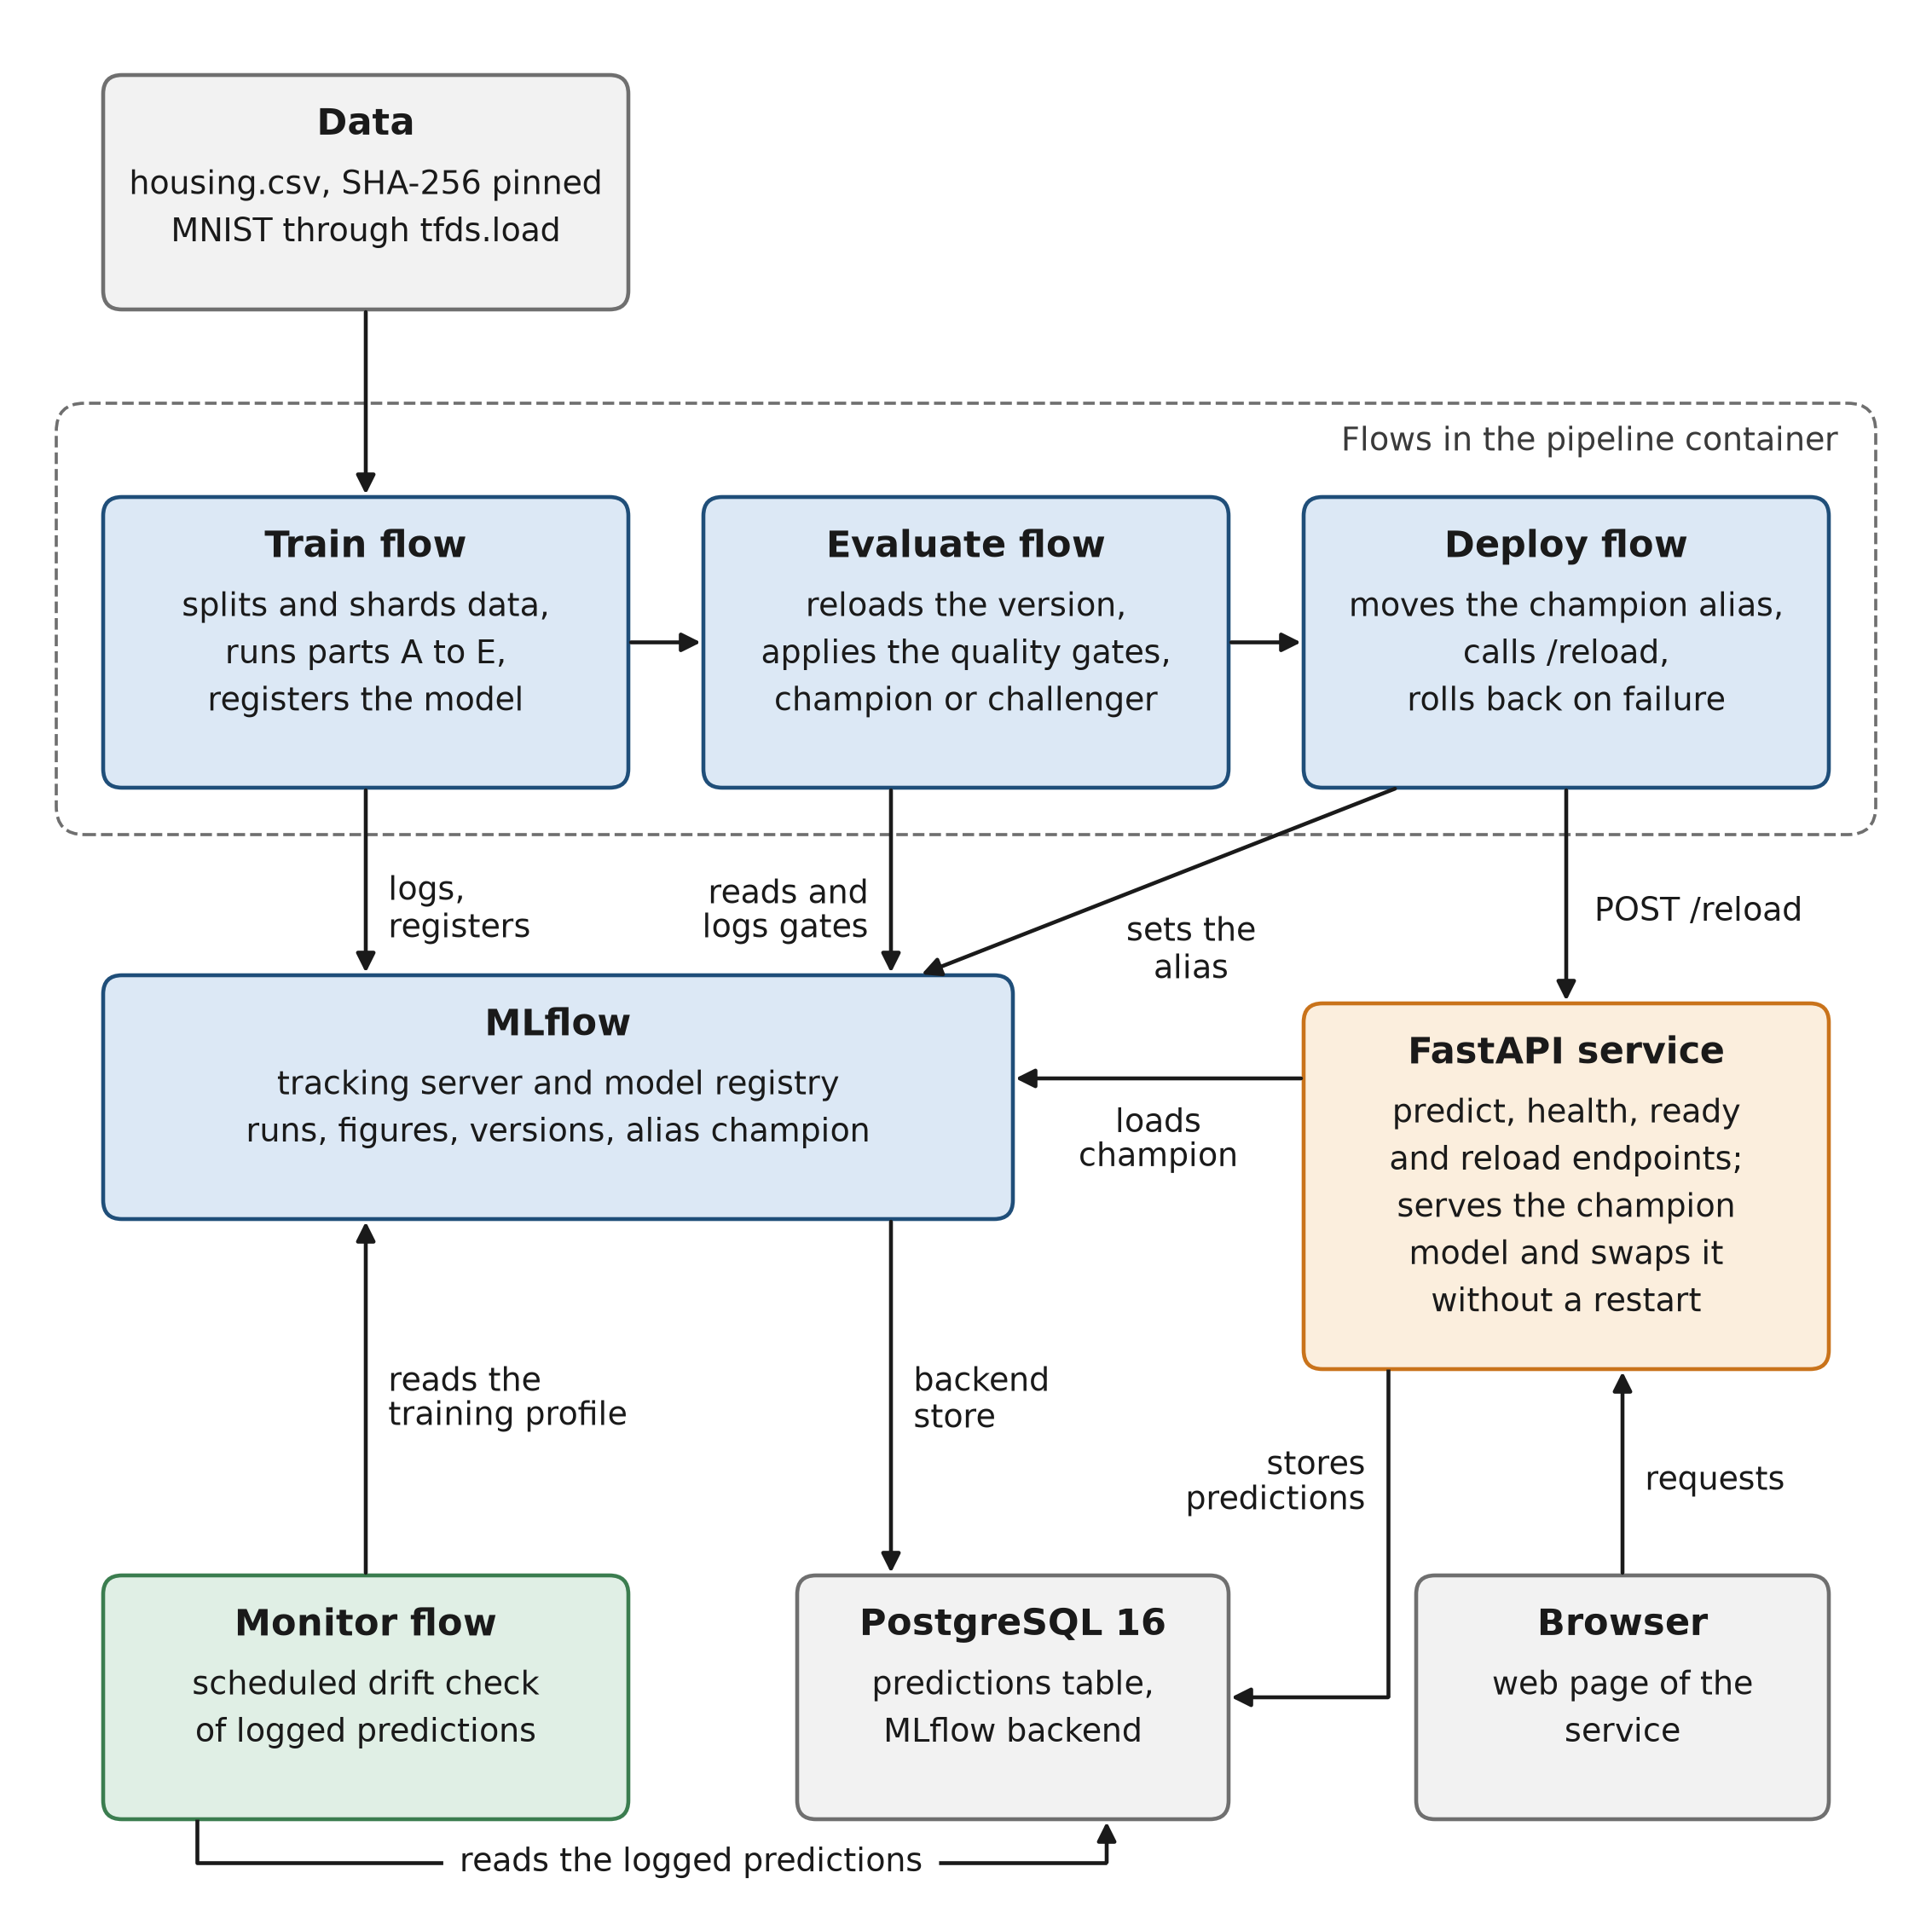
\includegraphics[width=\textwidth]{architecture.png}
\caption{Components of the system. Each arrow points from the component that calls to the component that it uses; the arrows between the three flows show the order in which they run.}
\label{fig:architecture}
\end{figure}

\subsection{Flows}

Four Prefect flows share one configuration file.

The \emph{train flow} prepares the data once, then runs Parts A to E as separate tasks. Every part writes its parameters, metrics and tables to its own nested MLflow run under one parent run. The model of Part E is registered in the MLflow Model Registry together with its lineage: the SHA-256 of the data, the MD5 of the configuration and the git commit (recorded as unknown for the run of this report, which was made outside a git checkout). At the end the flow writes the result tables, the figures and a summary of the run to the \texttt{reports} folder.

The \emph{evaluation flow} loads the registered candidate and re-evaluates it on the test rows that the training run had held out. A candidate passes only if it passes every one of the eight checks of Table~\ref{tab:gates}: five numerical thresholds, two checks of behaviour, and the comparison with the current champion, which may be at most a stated tolerance worse. The \emph{deploy flow} then gives the passing version the alias \texttt{champion} and asks the running service to reload it. The service must then report the new version and answer one canary request, a prediction for a held-out block. If it does not, the alias and the service return to the previous model, and a failed first deployment removes the alias again. When the service cannot be reached at all, the alias stays and the service loads it at its next start or registry check, unless the configuration requires the service, as it does in Docker; then the deployment is rolled back as well. Started alone, the deploy flow evaluates the candidate first, so a version that has not passed the checks is never promoted. The \emph{monitor flow} reads the logged predictions and reports requests that are unlike the training data: unseen categories, values outside the training range, missing values and shifts of the mean measured in training standard deviations.

\subsection{The pipeline that the book describes}

Figure~\ref{fig:pipeline} shows the two data paths of Parts A and B; the models of Parts C and E are trained from the second one. A set of shard files is listed in random order, and five files are open at the same time, their lines interleaved one at a time (the book's \texttt{n\_readers=5}). Whether these files are read by several threads is a separate setting, \texttt{n\_read\_threads}: it is \texttt{None} in the book's function, so the five files are read in turn, and \texttt{AUTOTUNE} in the pipelines that train the models of Parts C and E. A shuffle buffer mixes the lines. Each line is then parsed and standardised, the lines are collected into batches and the next batch is prepared while the current one is used. The right lane is the same idea on TFRecord files: each file is a GZIP-compressed sequence of serialised \texttt{tf.train.Example} messages, which can be parsed one batch at a time instead of one record at a time.

\begin{figure}[!htbp]
\centering
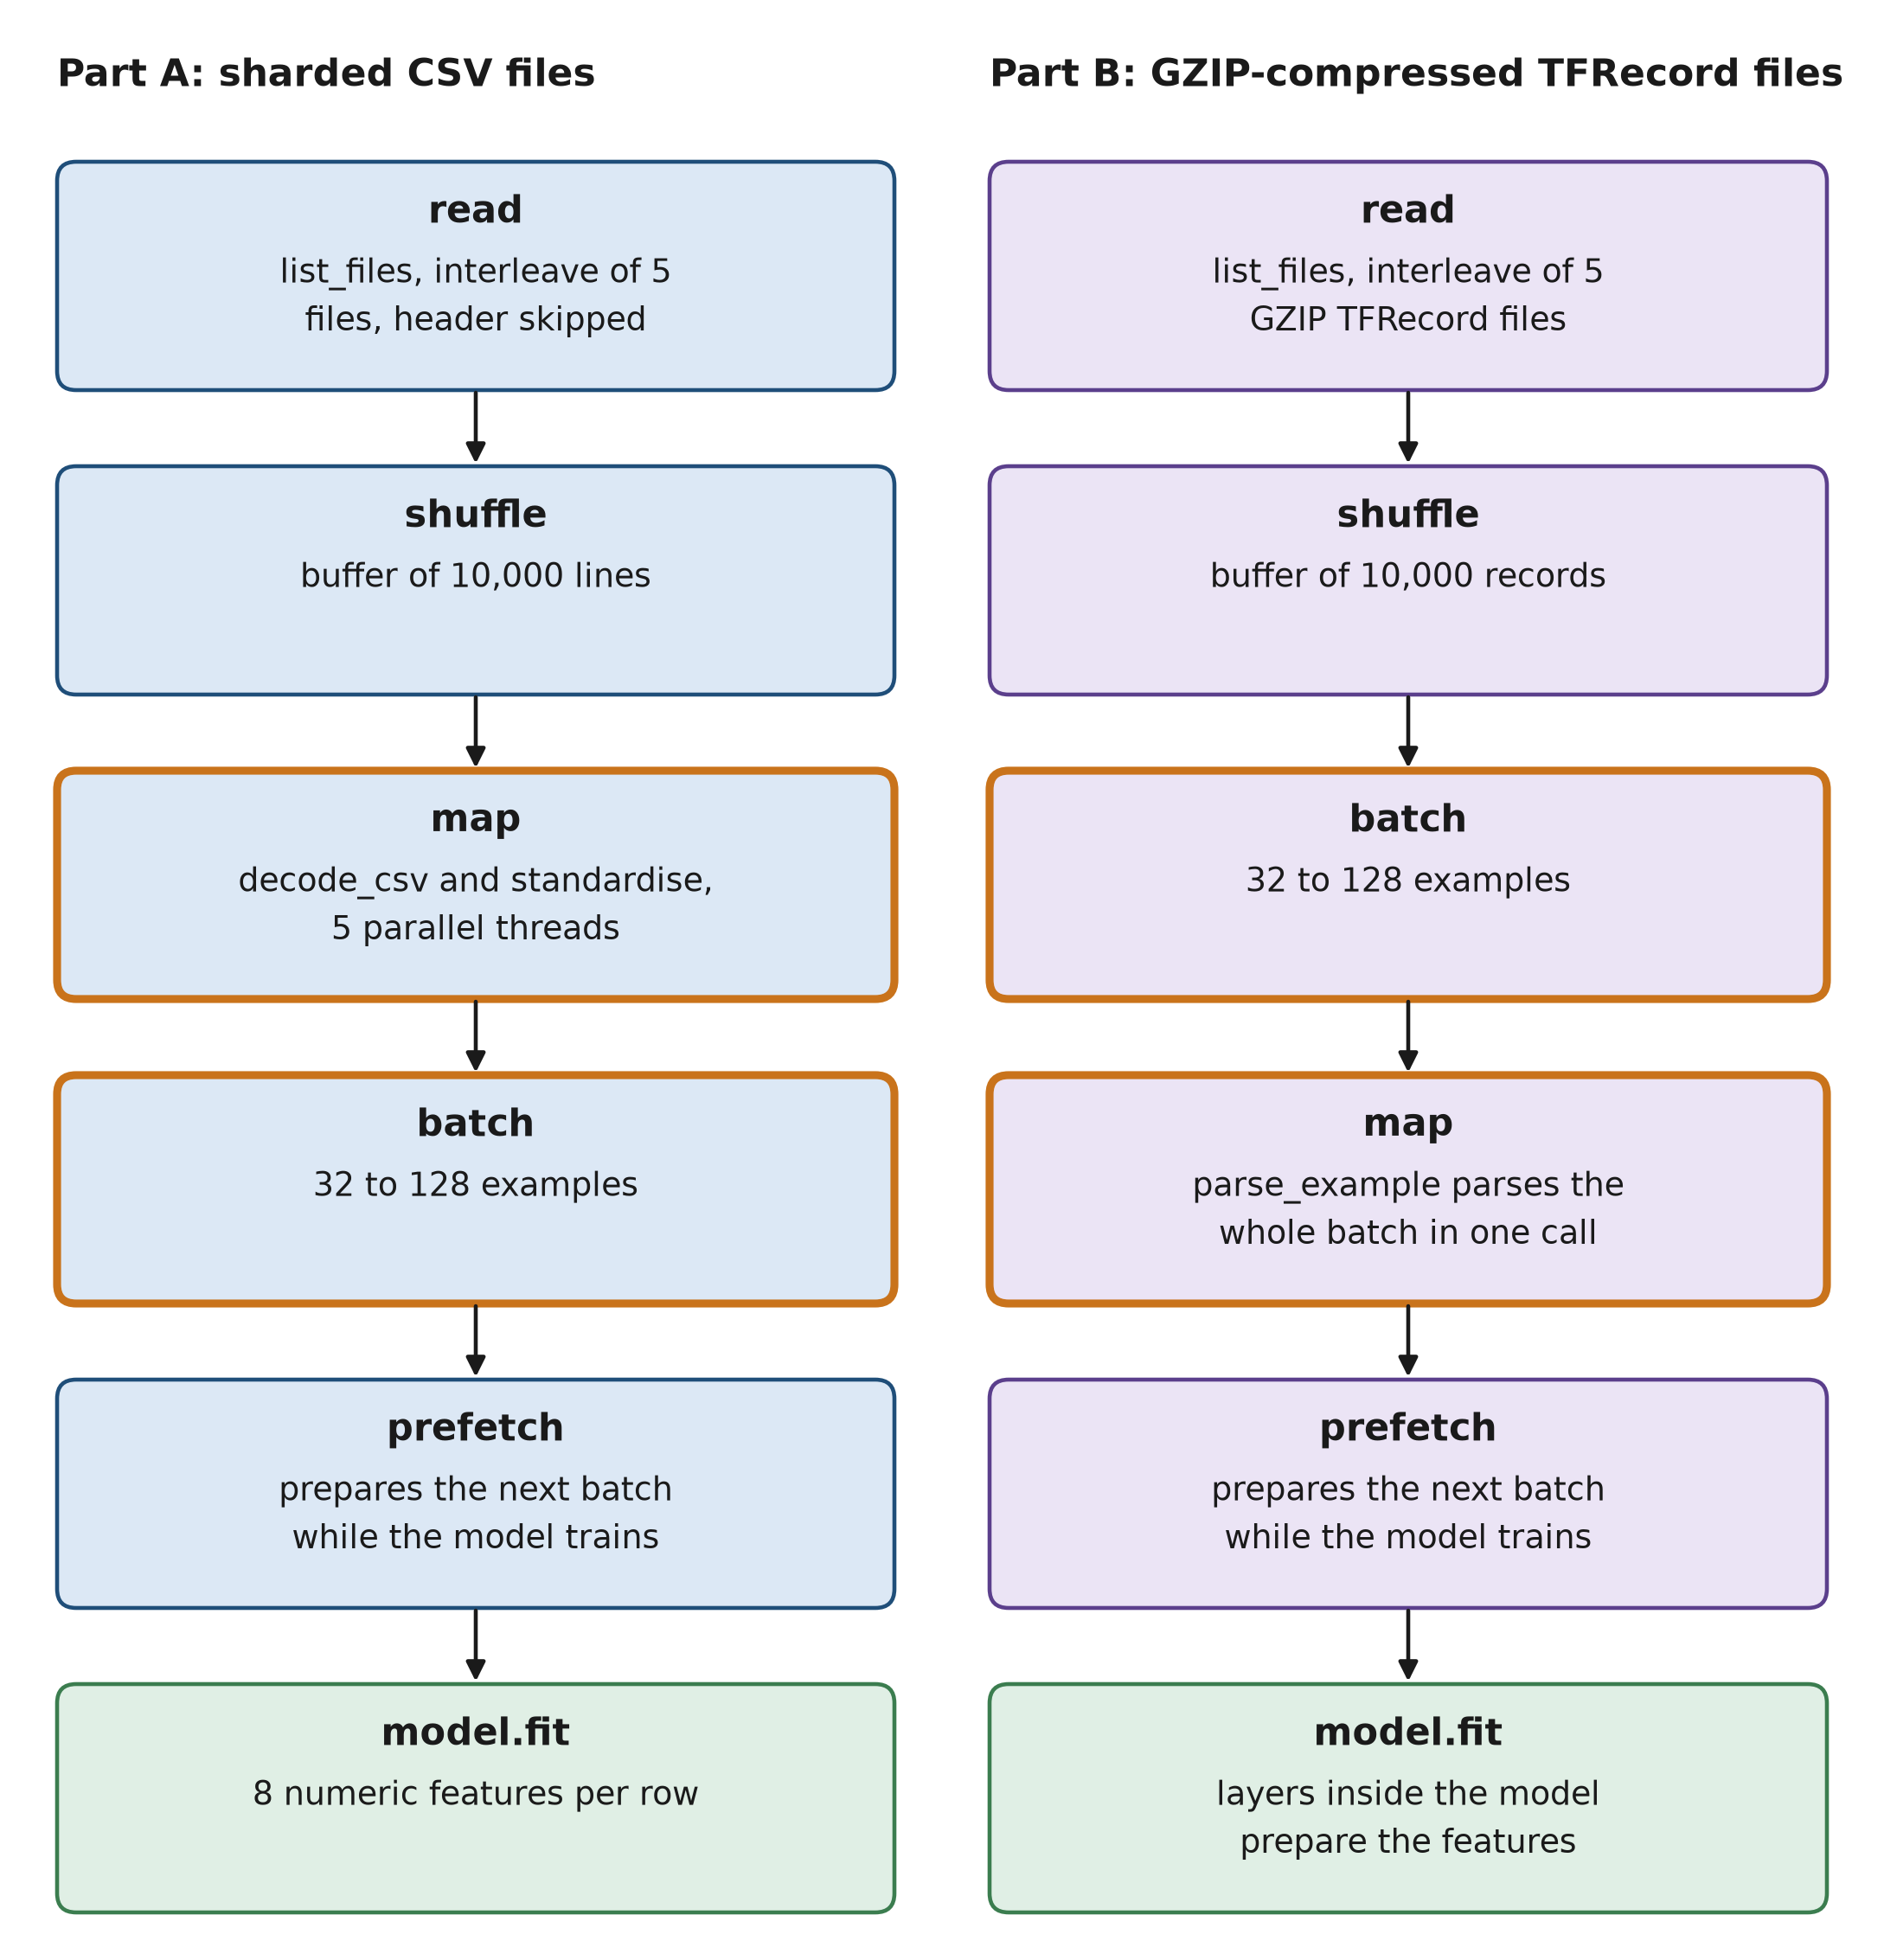
\includegraphics[width=\textwidth]{pipeline.png}
\caption{The two input pipelines. The left lane is the CSV pipeline of Part A and the right lane the TFRecord pipeline of Part B. Both end in \texttt{model.fit}. Orange edges mark the two steps that swap places between the lanes. Prefetch prepares the next batch in the background while the training step works on the current one.}
\label{fig:pipeline}
\end{figure}

\subsection{Tests and continuous integration}

The package has a test suite that runs without network access or a GPU: it checks the pipeline against pandas, the TFRecord size formula, the damaged-file detection, the equality of a dense layer on one-hot input with an embedding, the quality gates, the drift checks, the deploy flow (canary request and rollback) and the API (validation, reload and rollback). A GitHub Actions workflow runs the style checks and the tests on two Python versions, and then builds the Docker images, starts the stack, runs the whole flow with a reduced configuration and sends a request to the service. Section~\ref{sec:repro} gives the commands.

\section{Data and preparation}
\label{sec:data}

The data are the California housing census data that Chapter~2 of the book downloads. The file has 20,640 rows, one per census block group. There are eight numeric columns (longitude, latitude, median age of the houses, total rooms, total bedrooms, population, households and median income), one categorical column, \texttt{ocean\_proximity}, with the five values \texttt{<1H OCEAN}, \texttt{INLAND}, \texttt{ISLAND}, \texttt{NEAR BAY} and \texttt{NEAR OCEAN}, and the target, \texttt{median\_house\_value} in dollars. The column \texttt{total\_bedrooms} has 207 missing values. The file is taken from the book's own repository and is checked against two pinned SHA-256 digests (the archive and the CSV inside it), so a changed download is refused.

Chapter~2 of the book notes that the median house value, which is the target here, was capped, and its scatter plot of income against value shows the cap as a horizontal line at \$500,000. Of the \runSplitNTest{} test rows of this project, \val{cap:n} (\val{cap:pct}\%) have the largest value that occurs, \$\val{cap:value}. These rows are kept, and Section~\ref{sec:model} reports the error on them separately.

\paragraph{Split.} The rows are split as in Chapter~2: stratified on five income categories, so that all three parts have the same income distribution as the whole. First, 20\% of the rows, drawn at random within each income category, are held out as the test set. Of the remaining rows, 25\% are drawn in the same way as the validation set; this second split is a choice of the project and not of the book. The result is a 60/20/20 split with \runSplitNTrain{} training, \runSplitNValid{} validation and \runSplitNTest{} test rows. The validation set is used to compare feature sets in Part C; the test set is used only for the final model and for the quality gates.

\paragraph{Statistics from the training rows only.} A missing number is replaced by the training median of its column, as in Chapter~2, and numeric columns are standardised with the training mean and standard deviation. These statistics are computed once from the training rows and are never recomputed from the validation or the test rows. The target is divided by 100,000, so the model predicts hundreds of thousands of dollars and all errors are reported in dollars after multiplying back.

\paragraph{Shards.} The book recommends splitting a large file into several files of equal length, because files of equal length interleave best. The training rows are written to 20 CSV files, the validation rows to 10 and the test rows to 10, and the same rows are written in the same order to uncompressed and to GZIP-compressed TFRecord files. A shard never mixes rows of different splits. Floating-point numbers are written with their full precision and a missing value is written as an empty field, so that the CSV loses no information and the pipeline's own handling of missing values (Section~\ref{sec:csv}) is exercised on real gaps.

\section{Part A: the Data API on sharded CSV files}
\label{sec:csv}

\subsection{The pipeline}

The function \texttt{csv\_reader\_dataset} follows the one in the book. It lists the files in random order and repeats them, keeps five files open at the same time and interleaves their lines, one line from each file in turn (the book's \texttt{n\_readers=5}; each file's header is skipped), shuffles the lines in a buffer, parses each line with \texttt{tf.io.decode\_csv}, collects batches and prefetches. In the parsing step an empty field is replaced by the training median of its column, through the \texttt{record\_defaults} of \texttt{decode\_csv} (the book's defaults are 0; the median is a choice of this project that follows the imputer of Chapter~2), and the eight numbers are standardised with the training mean and standard deviation. The function has an argument for every step, so that each step can be switched off and measured. Reading threads are a separate argument, \texttt{n\_read\_threads}; the book notes that by default \texttt{interleave()} does not use parallelism, and its function leaves this argument at \texttt{None}, as do pipelines 1 to 5 below.

The first test is that the pipeline returns the same numbers as a plain pandas and NumPy computation of the same quantities. On the \val{eq:rows} training rows, of which \val{eq:missing} have a missing number, the largest absolute difference is \metric{A}{pipeline_max_abs_diff_inputs} in the inputs and \metric{A}{pipeline_max_abs_diff_targets} in the targets, which is consistent with the rounding of 32-bit floating-point numbers.

\subsection{Speed}

Each timing is the median of \param{A}{repeats} passes over the training rows (\val{sweep:batches} batches of \param{A}{batch_size}) after one warm-up pass. To see what a consumer that is not instantaneous does to the pipeline, each batch is followed by a simulated training step of 0 ms (reading only) or 4 ms. Two settings of \texttt{tf.data} are compared. In the first, \emph{only the listed steps}, the automatic graph optimisations of \texttt{tf.data} are switched off, so that a step is present only if the pipeline lists it. In the second, \emph{tf.data defaults}, they are left on. The first answers the question ``what does this step do'', the second ``what does a user get''.

Table~\ref{tab:csvspeed} and Figure~\ref{fig:csv} give the speed of six pipelines, each adding one step to the one above, and of the same computation done with pandas and NumPy. Each pass of this baseline reads the CSV shards into one data frame, standardises it and slices shuffled batches, so it holds all of the data in memory but also pays for reading and parsing the files.

\begin{table}[!htbp]
\centering
\small
\setlength{\tabcolsep}{4pt}
\begin{tabular}{L{6.2cm}R{1.95cm}R{1.95cm}R{1.95cm}R{1.95cm}}
\toprule
 & \multicolumn{2}{c}{No training step} & \multicolumn{2}{c}{4 ms training step} \\
\cmidrule(lr){2-3}\cmidrule(lr){4-5}
Pipeline & Only listed steps & tf.data defaults & Only listed steps & tf.data defaults \\
\midrule
1. one file, no shuffle, serial parse & 13,412 & 21,484 & 4,826 & 6,822 \\
2. + interleave 5 files & 15,632 & 19,019 & 4,792 & 6,851 \\
3. + shuffle buffer & 16,039 & 19,189 & 4,969 & 6,711 \\
4. + 5 parse threads & 18,935 & 25,885 & 5,275 & 6,686 \\
5. + prefetch(1), the book's function & 20,606 & 19,168 & 6,794 & 6,692 \\
6. + AUTOTUNE threads and prefetch & 15,525 & 15,104 & 6,646 & 6,612 \\
pandas and NumPy: read the shards, standardise, slice batches & 354,718 & 354,718 & 7,530 & 7,530 \\
\bottomrule
\end{tabular}

\caption{Examples read per second, without a training step and with a training step of 4~ms per batch. Row 5 is the function of the book.}
\label{tab:csvspeed}
\end{table}

\begin{figure}[!htbp]
\centering
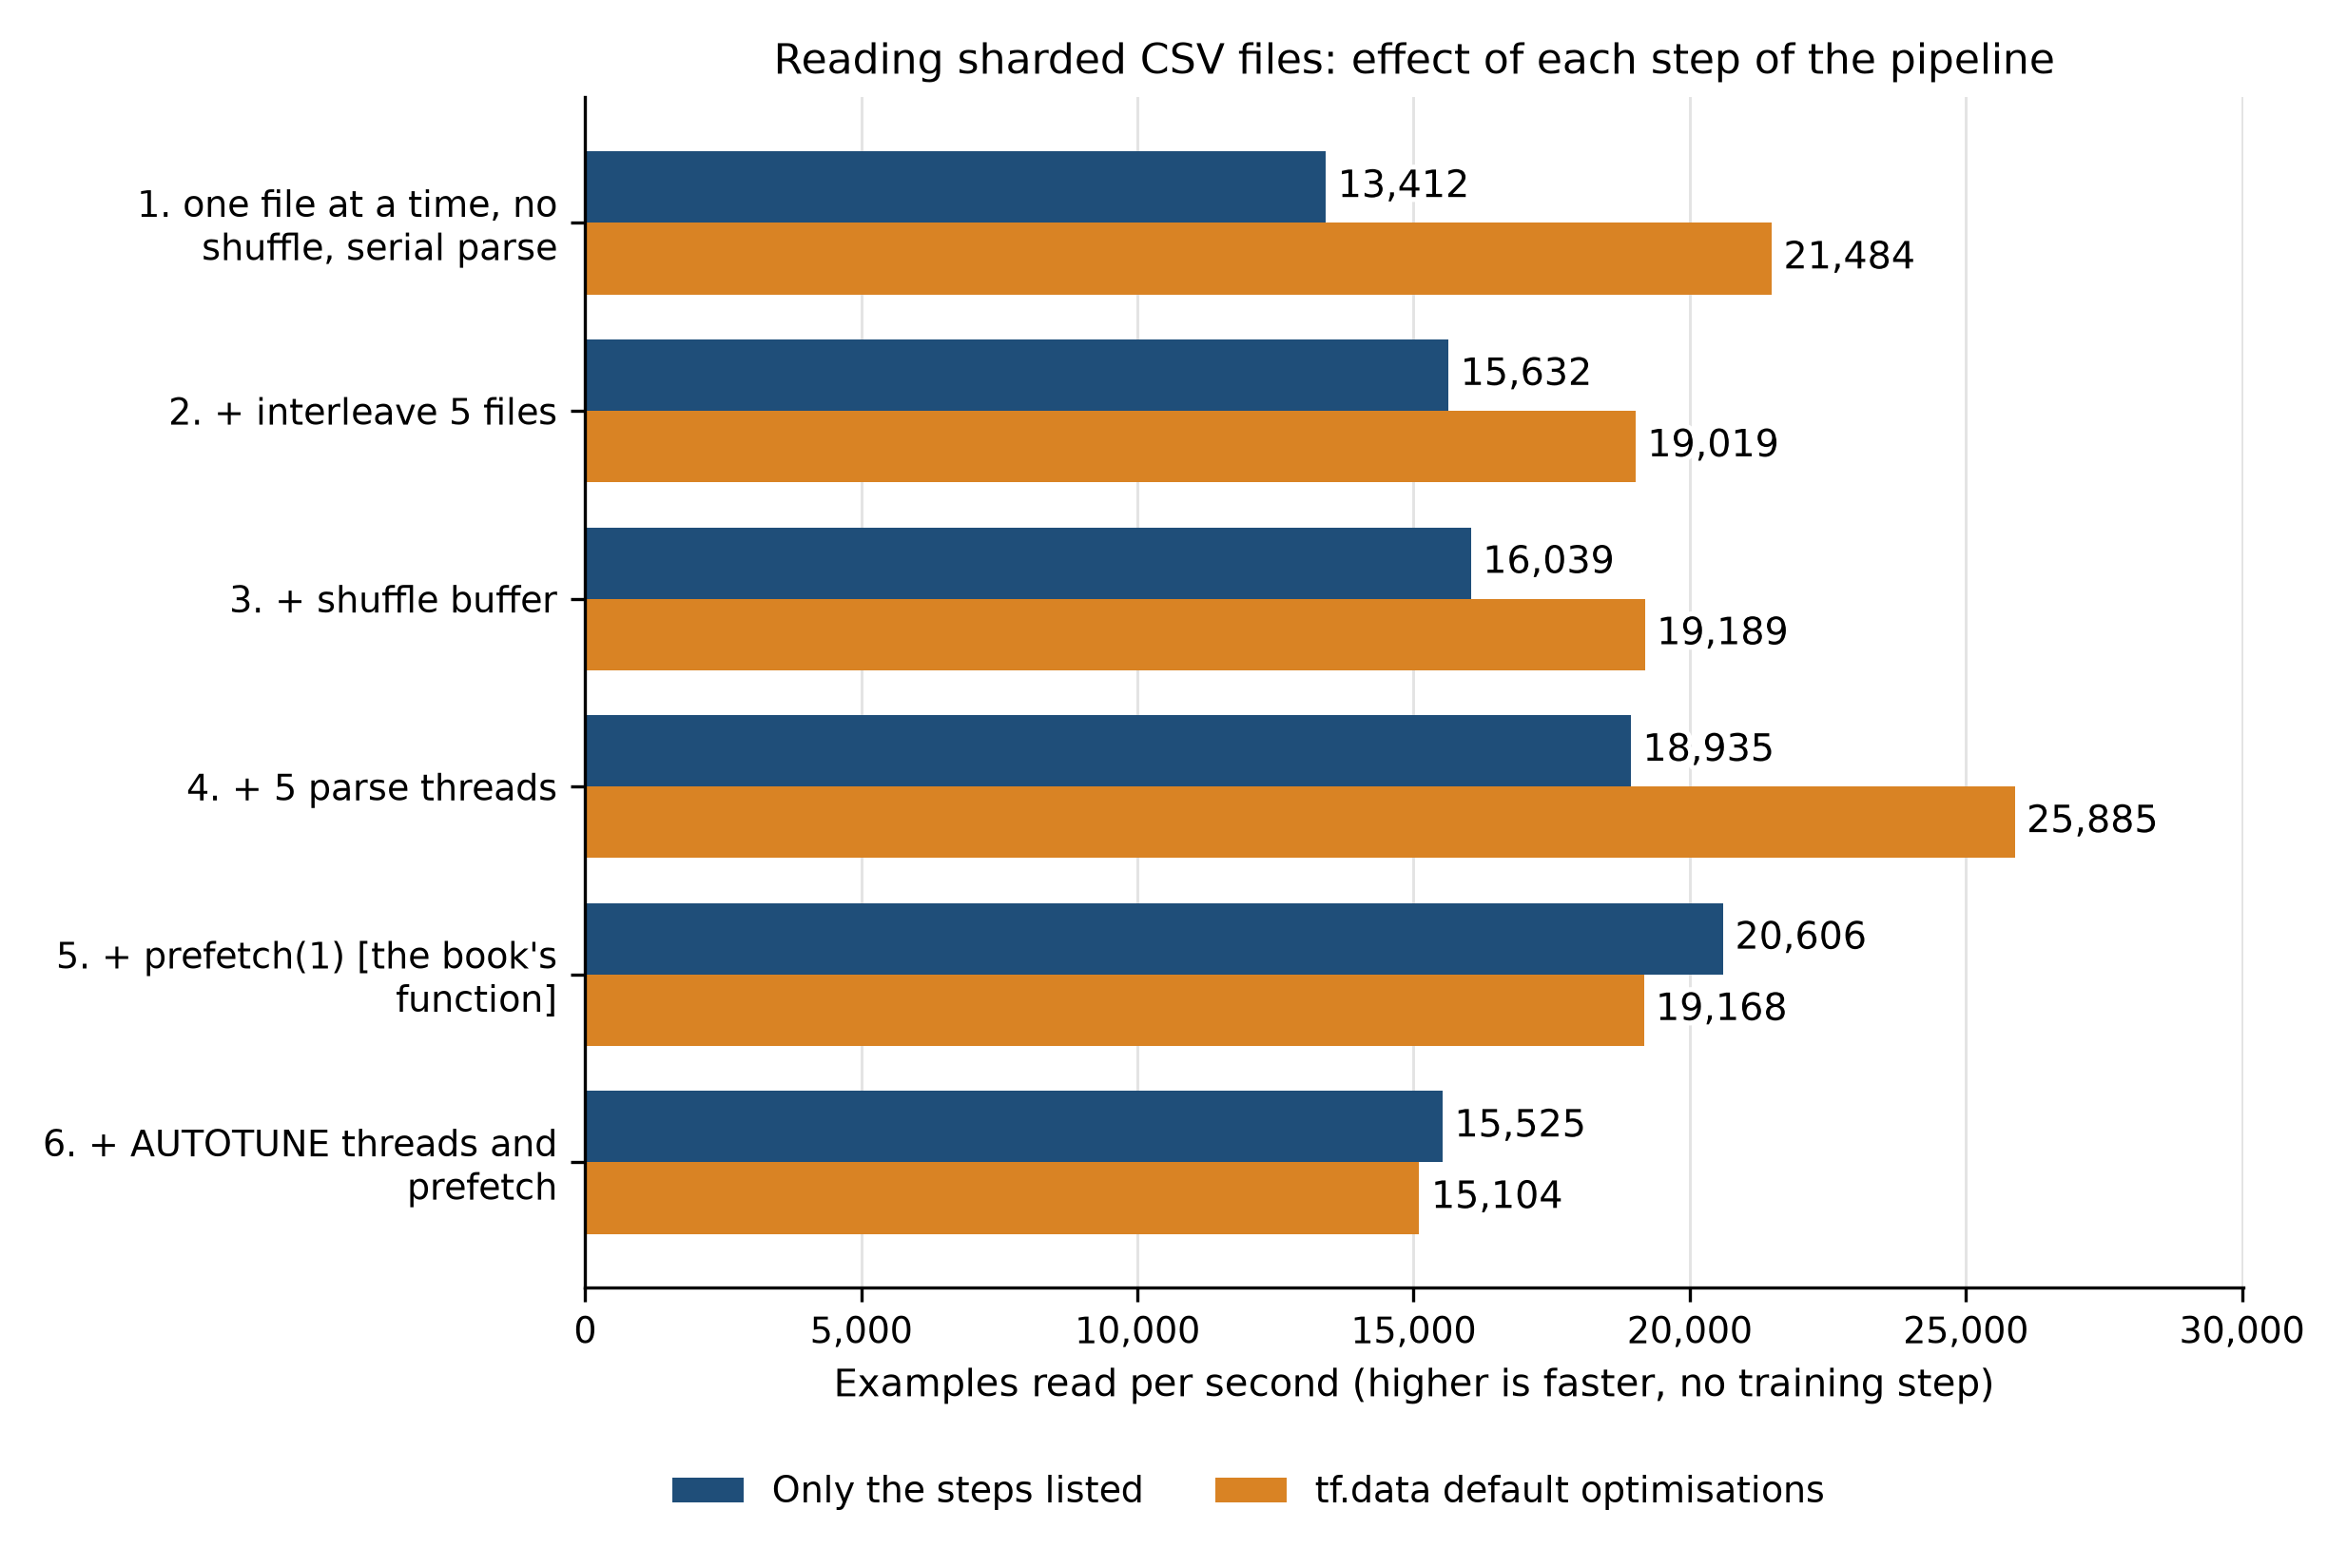
\includegraphics[width=0.92\textwidth]{a_csv_throughput.png}
\caption{Reading speed of the six pipelines of Table~\ref{tab:csvspeed}, without a training step.}
\label{fig:csv}
\end{figure}

With only the listed steps and no training step, the pipeline that reads one file at a time and parses serially reads \val{abl:strict:0:1} examples per second. Interleaving five files raises this to \val{abl:strict:0:2}, the shuffle buffer to \val{abl:strict:0:3}, five parsing threads to \val{abl:strict:0:4}, and \texttt{prefetch(1)}, which completes the function of the book, to \val{abl:strict:0:5}. The function of the book is therefore \val{ablr:strict:0:5:1} times as fast as the plain pipeline. The steps in between should not all be read as separate effects: each added step changes the speed by a factor of between \val{gain:strict:0:min} and \val{gain:strict:0:max}, and the noise of the measurement is of that order: within this run the same configuration was timed twice (row~6 with the \emph{tf.data defaults} in Table~\ref{tab:csvspeed}, and the CSV row of Table~\ref{tab:formats}) and gave \val{noise:a} and \val{noise:b} examples per second, \val{noise:pct}\% apart. Differences of that size or less between rows are therefore not treated as effects.

A training step makes prefetching matter. With a step of 4~ms the pipelines without prefetching read between \val{abl:strict:4:min14} and \val{abl:strict:4:max14} examples per second, and \texttt{prefetch(1)} raises the speed by a factor of \val{ablr:strict:4:5:4} to \val{abl:strict:4:5}. The ceiling for a step of 4~ms and batches of \param{A}{batch_size} is \val{bound:4} examples per second, because the step alone takes that long; the function of the book reaches \val{numpy:book:share:4}\% of the speed of the pandas and NumPy computation, \val{numpy:4} examples per second, in the same situation.

Two results are not what the book's description alone would lead one to expect. First, replacing the fixed values of the book (no reading threads, five parsing threads, \texttt{prefetch(1)}) by \texttt{tf.data.AUTOTUNE} for the reading threads, the parsing threads and the prefetching, with the same five interleaved files, did not help on this machine: without a training step it reads \val{abl:strict:0:6} examples per second, a ratio of \val{ablr:strict:0:6:5} to the fixed values, and with a step of 4~ms the ratio is \val{ablr:strict:4:6:5}. The machine has two cores, and I did not investigate the cause further. Second, in the \emph{tf.data defaults} setting the six pipelines are within \val{abl:default:4:spread}\% of each other when there is a training step (\val{abl:default:4:1} examples per second for the plainest and \val{abl:default:4:5} for the function of the book), and without a step the values, from \val{abl:default:0:min} to \val{abl:default:0:max}, do not form a monotone sequence. When the defaults are on, the plain pipeline is already as fast as the full one when there is a training step of 4~ms (a ratio of \val{ablr:default:4:5:1} for the function of the book to the plain pipeline), so the steps of the book show their effect when they are the only optimisation applied. This is why Table~\ref{tab:csvspeed} reports both settings.

The pandas and NumPy computation is faster than any of the streaming pipelines when there is no training step: it delivers \val{numpy:0} examples per second, \val{numpy:over:book:0} times the function of the book. This is a property of the small data set, whose training rows take only about 1~MB. The point of the pipeline is not to beat a computation that loads everything into memory but to keep working when the data no longer fit (Section~\ref{sec:tfrecord}, Table~\ref{tab:scale}).

\subsection{Prefetching and the formula}

Section~\ref{sec:math} shows that with \texttt{prefetch(1)} the time per batch is $\max(t_{\mathrm{in}}, t_{\mathrm{s}})$, where $t_{\mathrm{in}}$ is the time the input pipeline needs for a batch and $t_{\mathrm{s}}$ the time of the training step, and that without prefetching it is $t_{\mathrm{in}} + t_{\mathrm{s}}$. All of these runs read five interleaved files without reading threads and use a shuffle buffer of 10,000 lines, five parsing threads and no automatic optimisation (the \emph{only listed steps} setting), with and without \texttt{prefetch(1)}. The time $t_{\mathrm{in}}$ is measured with no training step and the formulas are then compared with the measurements for steps from 0 to 8~ms (Table~\ref{tab:prefetch}, Figure~\ref{fig:prefetch}).

\begin{table}[!htbp]
\centering
\small
\begin{tabular}{R{1.6cm}R{2.6cm}R{2.6cm}R{2.6cm}R{2.6cm}}
\toprule
Step (ms) & No prefetch, measured & No prefetch, formula & prefetch(1), measured & prefetch(1), formula \\
\midrule
0.0 & 1.66 & 1.66 & 1.64 & 1.66 \\
1.0 & 3.05 & 2.66 & 1.61 & 1.66 \\
2.0 & 4.04 & 3.66 & 2.66 & 2.00 \\
4.0 & 6.11 & 5.66 & 4.74 & 4.00 \\
8.0 & 10.25 & 9.66 & 8.76 & 8.00 \\
\bottomrule
\end{tabular}

\caption{Time per batch in milliseconds, measured and from the formulas of Section~\ref{sec:math}, with $t_{\mathrm{in}}$ taken from the measurement with a step of 0~ms.}
\label{tab:prefetch}
\end{table}

\begin{figure}[!htbp]
\centering
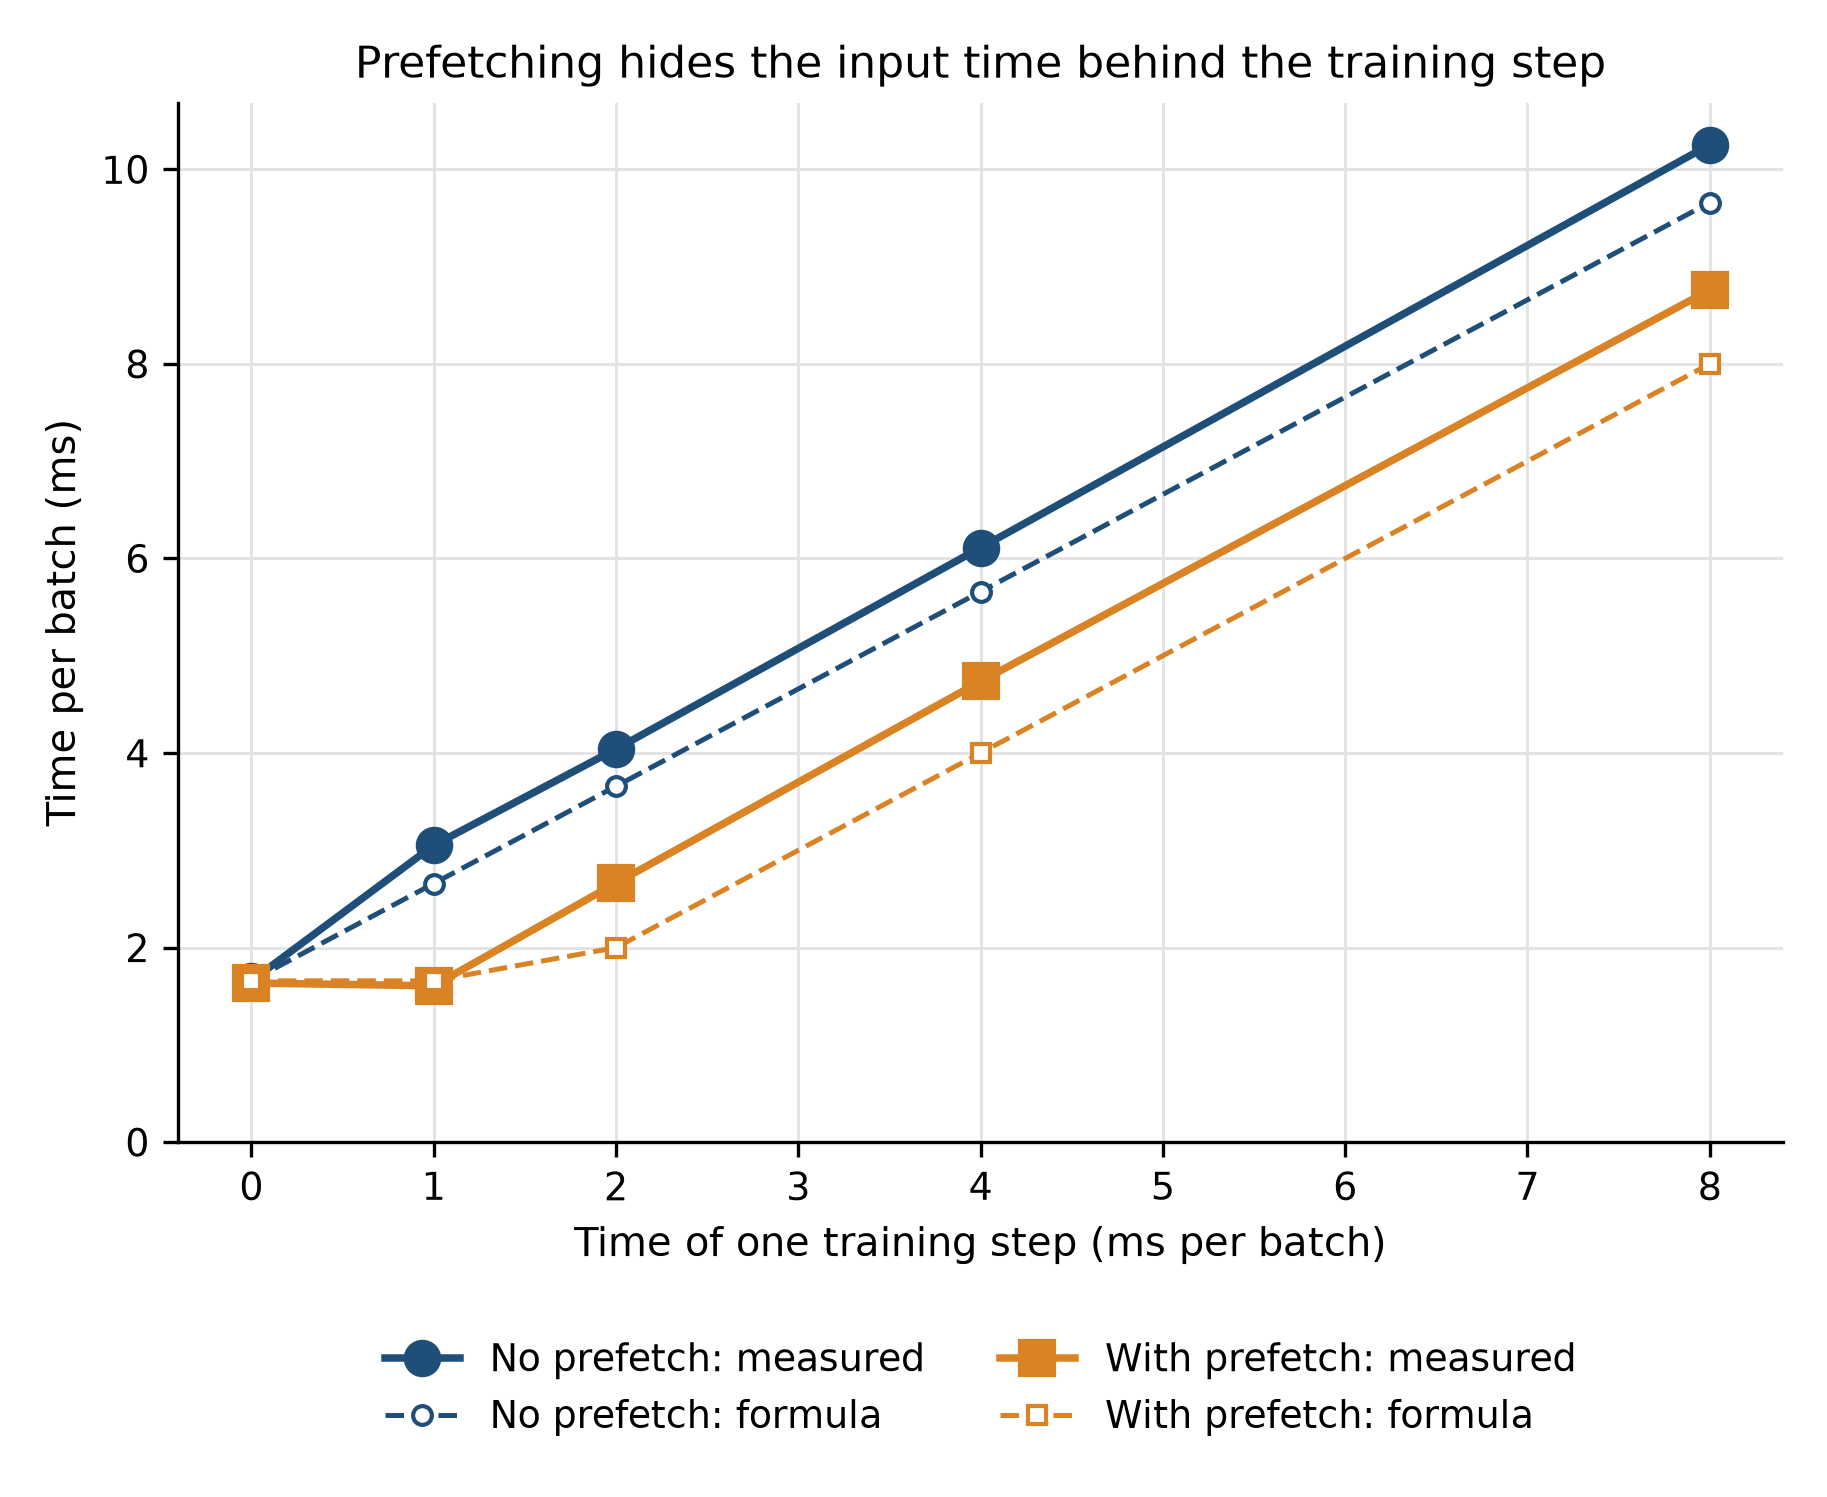
\includegraphics[width=0.92\textwidth]{a_prefetch_sweep.png}
\caption{Time per batch against the length of the training step, with and without prefetching. The dashed lines are the formulas. For a step of 0~ms the two measured series are nearly equal, so their markers overlap.}
\label{fig:prefetch}
\end{figure}

The shape of the formula is confirmed: with prefetching the time per batch stays at $t_{\mathrm{in}}$ as long as the step is shorter than $t_{\mathrm{in}}$ and then grows with a slope of one, and without prefetching it grows with a slope of one from the start. Without prefetching, the measured times exceed the formula by \val{sweep:serial:over:min} to \val{sweep:serial:over:max}~ms per batch for steps of 1~ms and more. With prefetching they agree with $t_{\mathrm{in}}$ for steps of 0 and 1~ms (\val{sweep:pf:0} and \val{sweep:pf:1}~ms against \val{sweep:pred:0}~ms) and exceed the formula by \val{sweep:over:min} to \val{sweep:over:max}~ms for steps of 2~ms and more. Possible reasons, which I did not test, are the cost of handing a batch from one thread to the other and the fact that a simulated step that sleeps for a given time takes a little longer than that time. Because the excess is almost constant, the conclusion of the formula, that prefetching saves the smaller of the two times per batch, holds.

\subsection{How well a shuffle buffer mixes sorted data}

Shuffling is tested on the worst case, a training set stored in sorted order. The training rows are sorted by the target, written to 20 files, and read with different pipelines, in batches of 64. The order correlation is the Spearman correlation between the position of an example in the stream and its target: 1 means the stream is still sorted, 0 means that the order is unrelated to the target. The batch diversity is defined in Section~\ref{sec:math}: 0 means that every batch contains almost the same targets, 1 that every batch looks like the whole set.

\begin{table}[!htbp]
\centering
\small
\begin{tabular}{L{4.4cm}R{1.4cm}R{1.4cm}R{1.8cm}R{1.8cm}R{2.4cm}}
\toprule
Shuffling & Readers & Buffer & Spearman & Formula & Batch diversity \\
\midrule
no shuffling & 1 & 0 & 1.000 &  & 0.006 \\
random file order only & 1 & 0 & $-$0.011 &  & 0.058 \\
interleave 5 files & 5 & 0 & 0.005 &  & 0.920 \\
buffer 100 & 1 & 100 & 1.000 & 1.000 & 0.033 \\
buffer 1000 & 1 & 1,000 & 0.965 & 0.963 & 0.267 \\
buffer 10000 & 1 & 10,000 & 0.061 &  & 0.974 \\
interleave 5 + buffer 100 & 5 & 100 & 0.005 &  & 0.916 \\
interleave 5 + buffer 1000 & 5 & 1,000 & 0.006 &  & 0.943 \\
interleave 5 + buffer 10000 & 5 & 10,000 & $-$0.010 &  & 0.987 \\
\bottomrule
\end{tabular}

\caption{Reading sorted data. ``Formula'' is the prediction of Section~\ref{sec:math}, which is compared with the measurement only for buffers of at most a quarter of the \val{eq:rows} rows (here 100 and 1,000). The rows with ``random file order'' or ``interleave'' also shuffle the order of the files; the rows ``buffer'' alone do not. ``Readers'' is the number of files interleaved (\texttt{n\_readers}); none of these pipelines uses reading or parsing threads.}
\label{tab:shuffle}
\end{table}

\begin{figure}[!htbp]
\centering
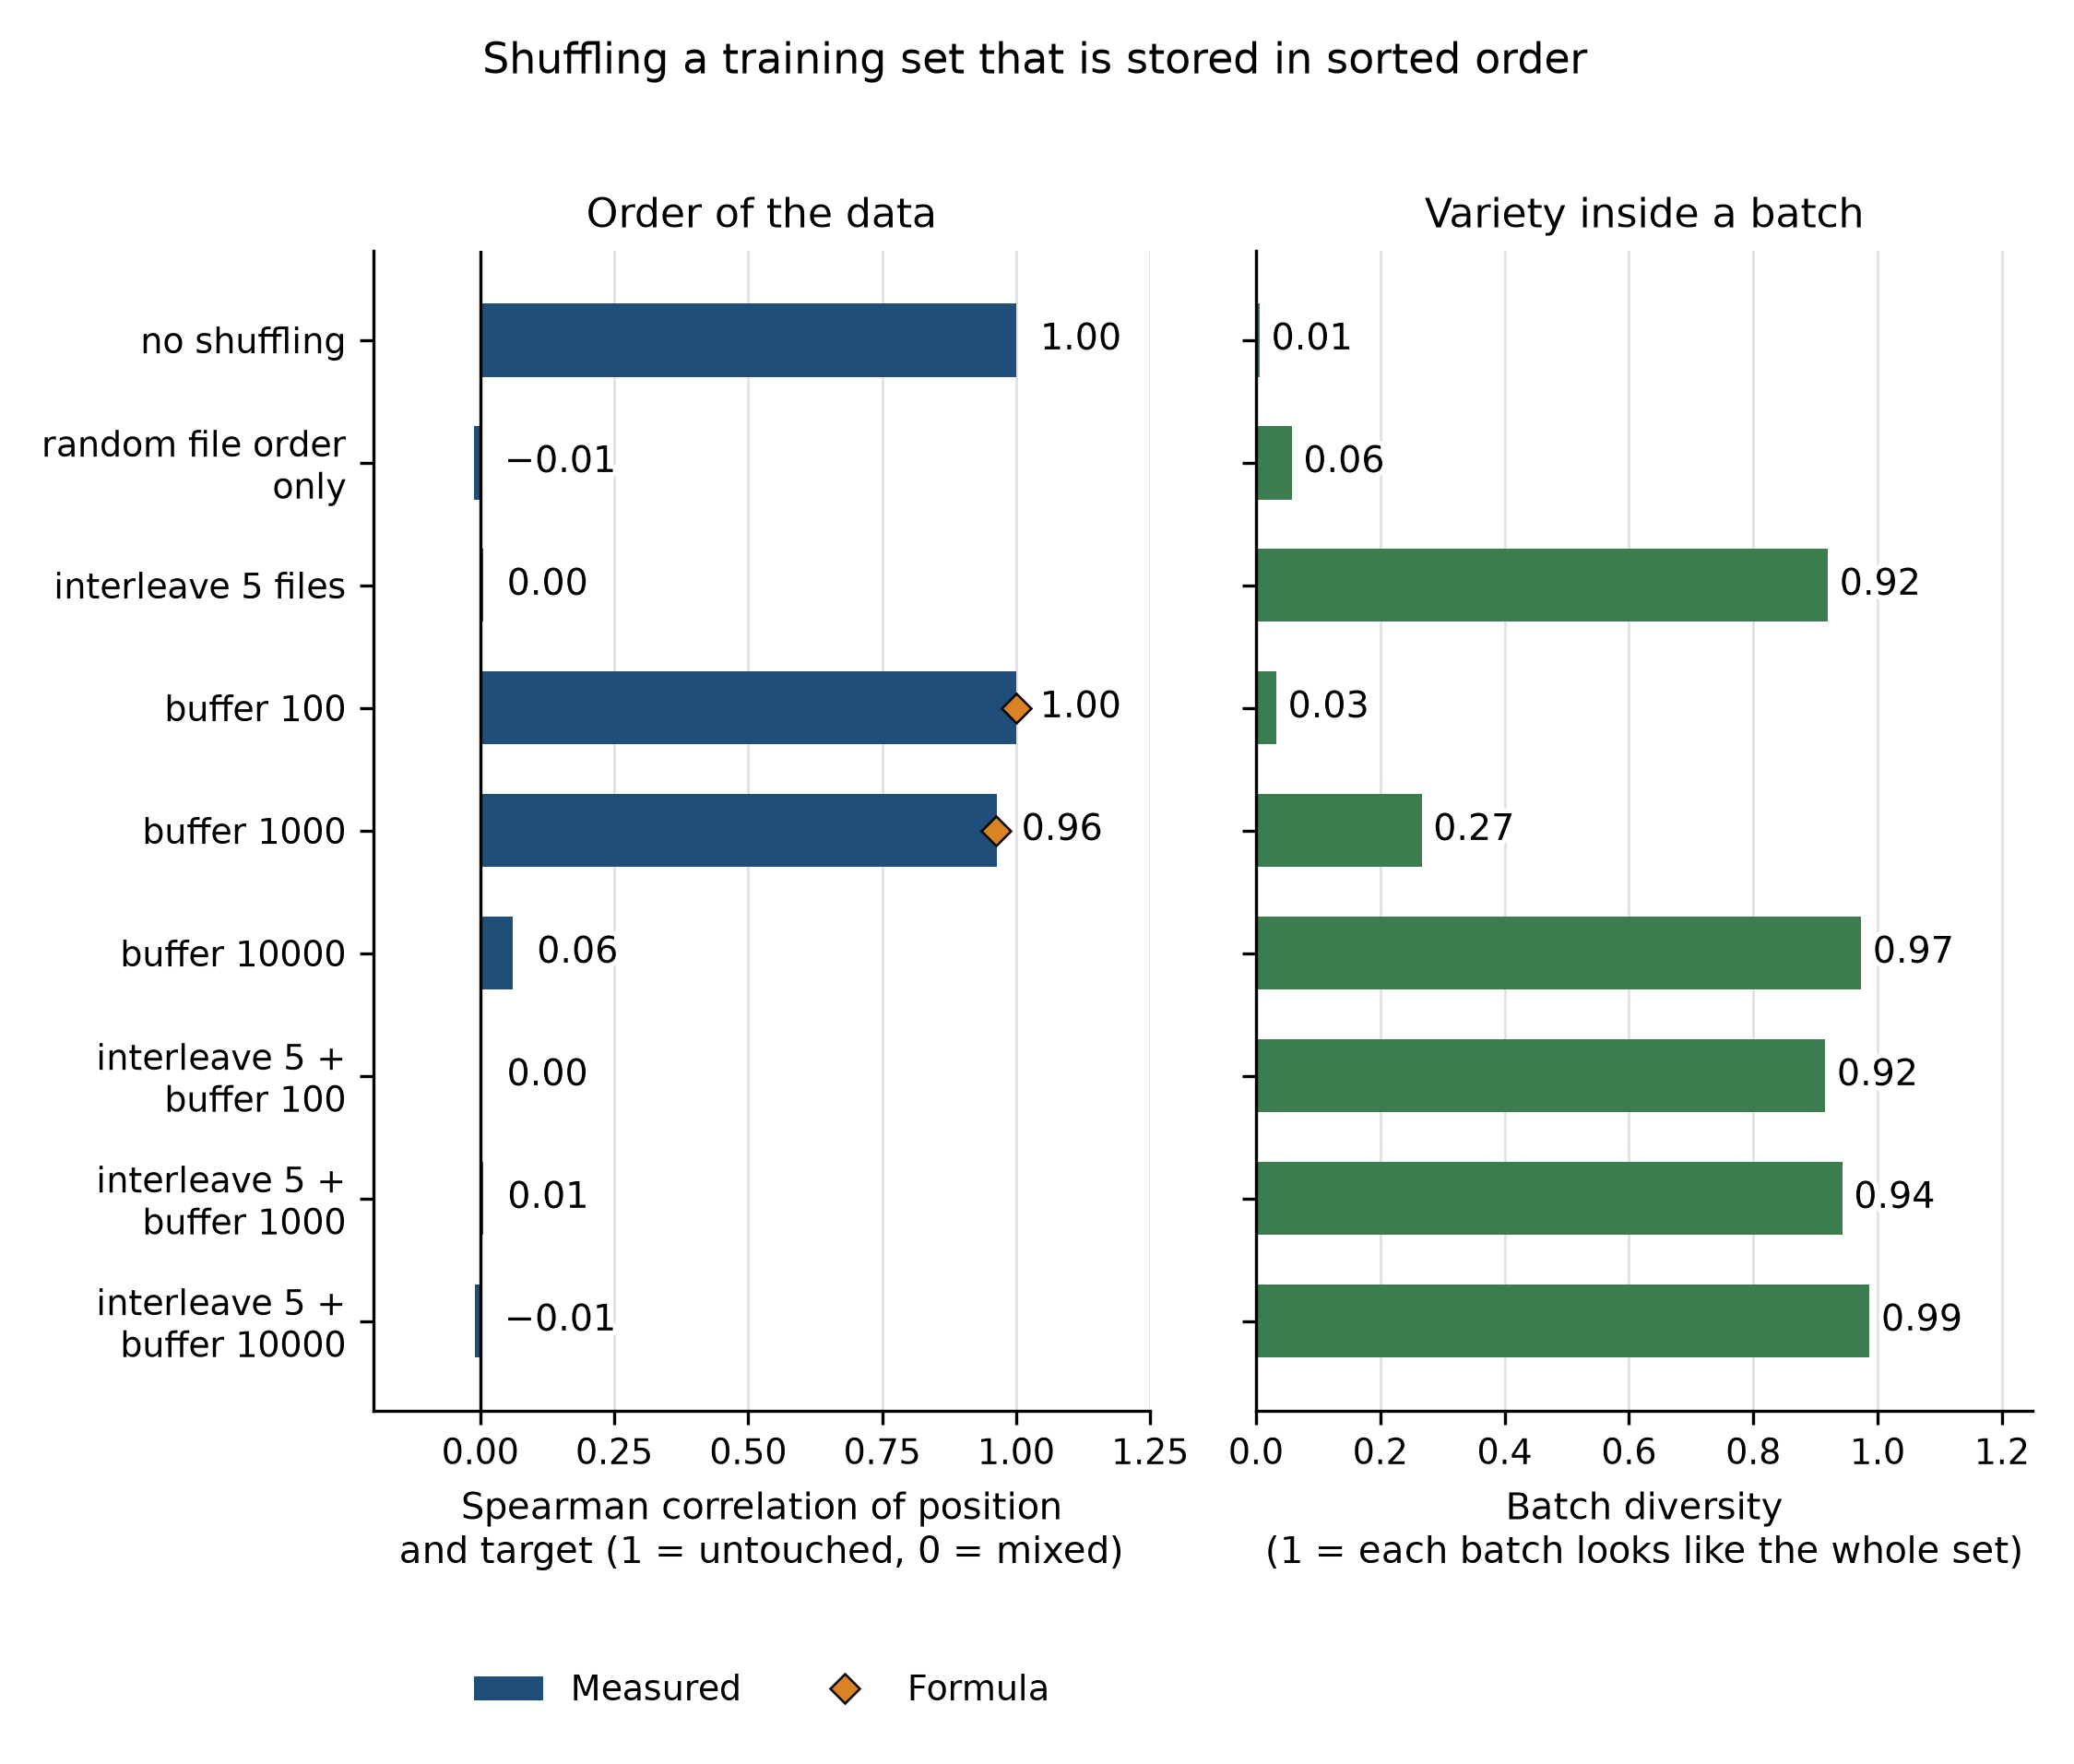
\includegraphics[width=\textwidth]{a_shuffle_quality.png}
\caption{Order correlation (left) and batch diversity (right) for the pipelines of Table~\ref{tab:shuffle}. The diamonds on the left are the predictions of the formula.}
\label{fig:shuffle}
\end{figure}

A buffer of 100 rows leaves sorted data almost sorted (correlation \val{shuf:buffer-100:rho}, formula \val{shuf:buffer-100:pred}), and a buffer of 1,000 rows leaves it mostly sorted (\val{shuf:buffer-1000:rho} against the predicted \val{shuf:buffer-1000:pred}). In the \val{shuf:npred} cases in which the formula was compared with the measurement the largest difference is \val{shuf:maxdev}. A buffer of 10,000 rows is \val{shuf:buf10000:frac}\% of the data, beyond the quarter up to which the formula is compared, and reduces the correlation to \val{shuf:buffer-10000:rho}.

The correlation alone can mislead. Reading the files in random order, with no buffer, gives a correlation of \val{shuf:random-file-order-only:rho}, which looks like perfect shuffling, but the batch diversity is only \val{shuf:random-file-order-only:div}: each file is still sorted, so every batch holds almost the same targets. Interleaving five files at once, as the book does, gives a diversity of \val{shuf:interleave-5-files:div} already and, together with a buffer of 10,000 rows, \val{shuf:interleave-5-buffer-10000:div}. This is the reason for the two steps of the book: the shuffling of the file order and the interleaving mix the data coarsely, the buffer mixes it finely.

\section{Part B: the TFRecord format}
\label{sec:tfrecord}

\subsection{From CSV to TFRecord}

A TFRecord file is a sequence of binary records, and each record here is one serialised \texttt{tf.train.Example}: a Protocol Buffers message that maps feature names to a list of floats, of integers or of byte strings. A housing row becomes an \texttt{Example} with ten features: the eight numbers and the target as float lists of one element, and \texttt{ocean\_proximity} as a byte string. A missing number is not written. The rows are written in the same order and into the same number of files as the CSV shards, once uncompressed and once with GZIP compression (\texttt{tf.io.TFRecordOptions}).

Reading uses \texttt{tf.io.FixedLenFeature} for every feature. A missing number then gets its \emph{default value}, which is set to the training median, exactly as for the CSV pipeline; a test checks that the value that comes out of a record without \texttt{total\_bedrooms} is the training median. The target has no default, so a record without a target raises an error.

The CSV and the TFRecord pipelines return the same data: the largest absolute difference between the numbers they produce is \metric{B}{csv_tfrecord_max_abs_diff}, the categories are equal, and the compressed files hold the same records as the uncompressed ones.

\subsection{The size of a file can be computed}

Section~\ref{sec:math} derives the number of bytes of a serialised \texttt{Example} and of a file from the Protocol Buffers encoding. The experiment computes this number for each of the \val{eq:rows} training rows from its values alone, without writing anything, and compares it with the real length. Table~\ref{tab:wire} shows that every record, and therefore the whole file, has exactly the predicted size. The records have between \val{wire:min} and \val{wire:max} bytes; the differences come from the missing numbers, which are left out, and from the length of the category name.

\begin{table}[!htbp]
\centering
\small
\begin{tabular}{p{9cm}r}
\toprule
Quantity & Value \\
\midrule
Records & 12,384 \\
Serialised Example, smallest and largest (bytes) & 243 and 275 \\
Serialised Example, mean (bytes) & 272.79 \\
File size from the formula (bytes) & 3,576,363 \\
File size on disk (bytes) & 3,576,363 \\
Formula equals the length of every record & yes \\
\bottomrule
\end{tabular}

\caption{The size of the uncompressed TFRecord file of the training rows, predicted and measured.}
\label{tab:wire}
\end{table}

\subsection{Size and reading speed}

Table~\ref{tab:formats} and Figure~\ref{fig:formats} compare five ways of storing and reading the same \val{eq:rows} training rows: the CSV shards, the same shards compressed with GZIP, TFRecord shards parsed one record at a time (\texttt{tf.io.parse\_single\_example}), TFRecord shards parsed a batch at a time (\texttt{tf.io.parse\_example} after \texttt{batch}), and the compressed TFRecord shards parsed a batch at a time. All five use the same settings: five interleaved files, a shuffle buffer of 10,000 examples, \texttt{tf.data.AUTOTUNE} for the reading and parsing threads and for prefetching, one pass and no training step.

\begin{table}[!htbp]
\centering
\small
\begin{tabular}{L{7.0cm}R{2.2cm}R{2.0cm}R{2.6cm}}
\toprule
Format and reading & Bytes & Size vs CSV & Examples per second \\
\midrule
csv & 856,778 & 1.00 & 16,602 \\
csv.gz & 287,248 & 0.34 & 16,405 \\
tfrecord, parse one record at a time & 3,576,363 & 4.17 & 17,964 \\
tfrecord, parse a batch at a time & 3,576,363 & 4.17 & 60,155 \\
tfrecord.gz, parse a batch at a time & 483,662 & 0.56 & 62,195 \\
\bottomrule
\end{tabular}

\caption{Size and reading speed of the same training rows in five formats.}
\label{tab:formats}
\end{table}

\begin{figure}[!htbp]
\centering
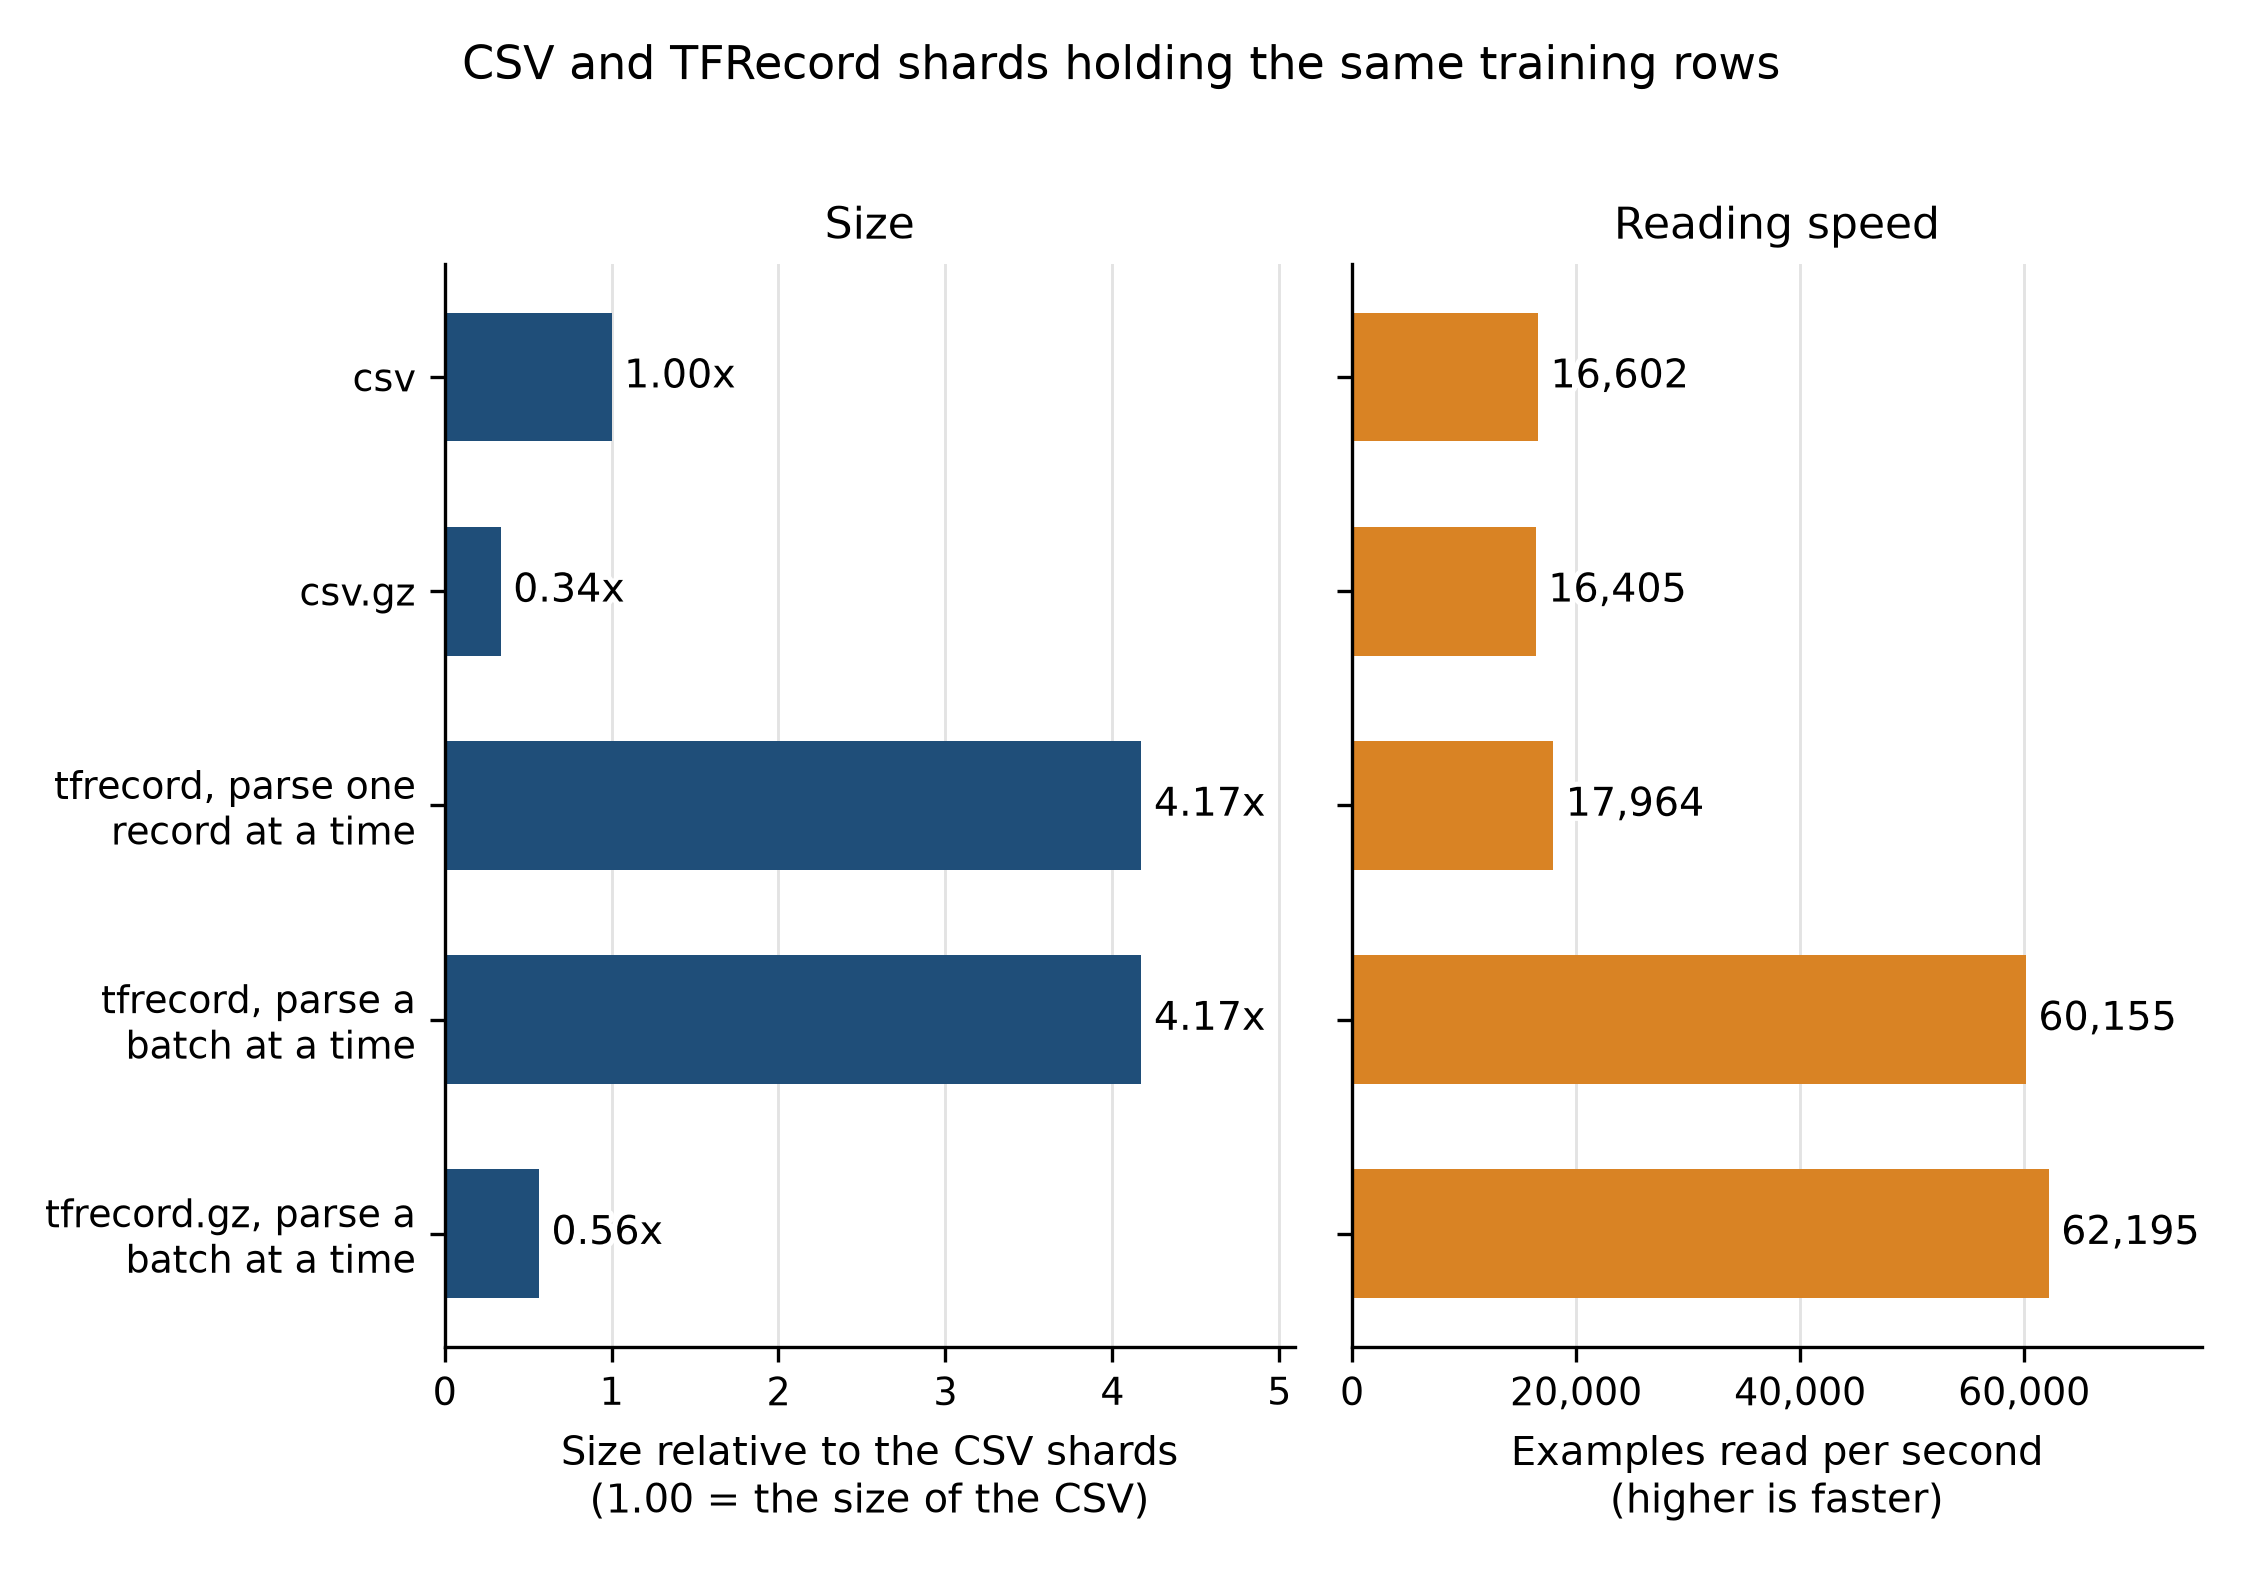
\includegraphics[width=\textwidth]{b_formats.png}
\caption{Size (left) and reading speed (right) of the five formats of Table~\ref{tab:formats}.}
\label{fig:formats}
\end{figure}

\paragraph{Size.} An uncompressed TFRecord is \val{fmt:tfr:size} times as large as the CSV, because every record repeats the names of its ten features and adds the framing and the type information of the message, whereas a CSV states the names once in the header. Compression removes this repetition: the GZIP TFRecord is \val{fmt:tfrgz:size} times the size of the CSV. The comparison with the CSV is not the fair one, though. A GZIP-compressed CSV is only \val{fmt:csvgz:size} times the size of the CSV, so the compressed TFRecord is \val{fmt:tfrgz:over:csvgz} times as large as the compressed CSV. TFRecord does not win on size for these data, and the report does not claim that it does.

\paragraph{Speed.} Parsing one record at a time is as fast as reading the CSV (\val{fmt:single:over:csv} times the speed of the CSV, which is within the noise of Section~\ref{sec:csv}). The gain comes from parsing a whole batch of serialised records in one call: it is \val{fmt:batch:over:csv} times as fast as the CSV, and \val{fmt:batch:over:single} times as fast as parsing record by record. The CSV pipeline parses one line per call; a CSV reader that parses a whole batch of lines with one call was not tested, so the factor of \val{fmt:batch:over:csv} does not separate the effect of the format from the effect of batching. All five rows use \texttt{tf.data.AUTOTUNE}, which Section~\ref{sec:csv} found slower than fixed thread counts on this machine, and the ratios were not measured again with fixed counts. The compressed files are read as fast as the uncompressed ones (\val{fmt:batchgz:over:csv} times the speed of the CSV), so on this machine the decompression is not a cost that shows in the measurement.

\subsection{Damaged files are detected}

Every record carries two CRC checksums, one for its length and one for its data (Section~\ref{sec:math}). Table~\ref{tab:corruption} shows what happens when a file that reads correctly is damaged in the middle (one byte flipped) or cut off at 60\% of its length. In all \val{corr:cases} cases tested, for both the uncompressed and the compressed file, reading stops with a \texttt{DataLossError} instead of delivering wrong numbers. In the uncompressed file the flipped byte is caught by the checksums of the record; for the compressed file the test does not show whether the error came from the checksums of the records or from the decompression. This is the result of the run reported here and not a guarantee: the byte at which a file is cut depends on the order in which Protocol Buffers writes the features, and in about one test process in forty a compressed file that was cut at 60\% was read to its end as a shorter file without an error. A pipeline that must not lose records therefore compares the number of records read with the number written, in addition to relying on the checksums.

\begin{table}[!htbp]
\centering
\small
\begin{tabular}{llll}
\toprule
File & Case & Result & Error raised \\
\midrule
uncompressed & intact & read 620 records & no \\
uncompressed & one byte flipped in the middle & DataLossError & yes \\
uncompressed & truncated at 60\% & DataLossError & yes \\
GZIP & intact & read 620 records & no \\
GZIP & one byte flipped in the middle & DataLossError & yes \\
GZIP & truncated at 60\% & DataLossError & yes \\
\bottomrule
\end{tabular}

\caption{Reading an intact and a damaged shard of 620 records.}
\label{tab:corruption}
\end{table}

\subsection{Scaling up}

The training set is only about 1~MB, so the interesting question is what the two approaches cost when the data are larger. The training shards are repeated $N$ times, for $N = 1$, 10 and 100, giving up to \val{scale:rows:max} rows and \val{scale:csv:max}~MB of CSV, and two ways of reading them are compared, each in a fresh process: one pass through the compressed TFRecord shards with the \texttt{tf.data} pipeline (shuffle buffer of 10,000 examples, batches of \param{B}{batch_size}), and loading all CSV shards into a pandas data frame and standardising it. The memory growth is the increase of the resident memory of the process during the pass.

\begin{table}[!htbp]
\centering
\small
\setlength{\tabcolsep}{4pt}
\begin{tabular}{R{1.2cm}R{1.8cm}R{1.4cm}R{2.1cm}R{1.7cm}R{1.7cm}R{1.6cm}R{1.6cm}}
\toprule
Copies & Rows & CSV (MB) & TFRecord.gz (MB) & tf.data growth (MB) & pandas growth (MB) & tf.data pass (s) & pandas load (s) \\
\midrule
1 & 12,384 & 0.9 & 0.5 & 11 & 8 & 0.2 & 0.0 \\
10 & 123,840 & 8.5 & 4.7 & 26 & 34 & 1.9 & 0.2 \\
100 & 1,238,400 & 85.4 & 47.2 & 31 & 182 & 20.5 & 1.1 \\
\bottomrule
\end{tabular}

\caption{Memory and time of one pass over the training set repeated $N$ times.}
\label{tab:scale}
\end{table}

\begin{figure}[!htbp]
\centering
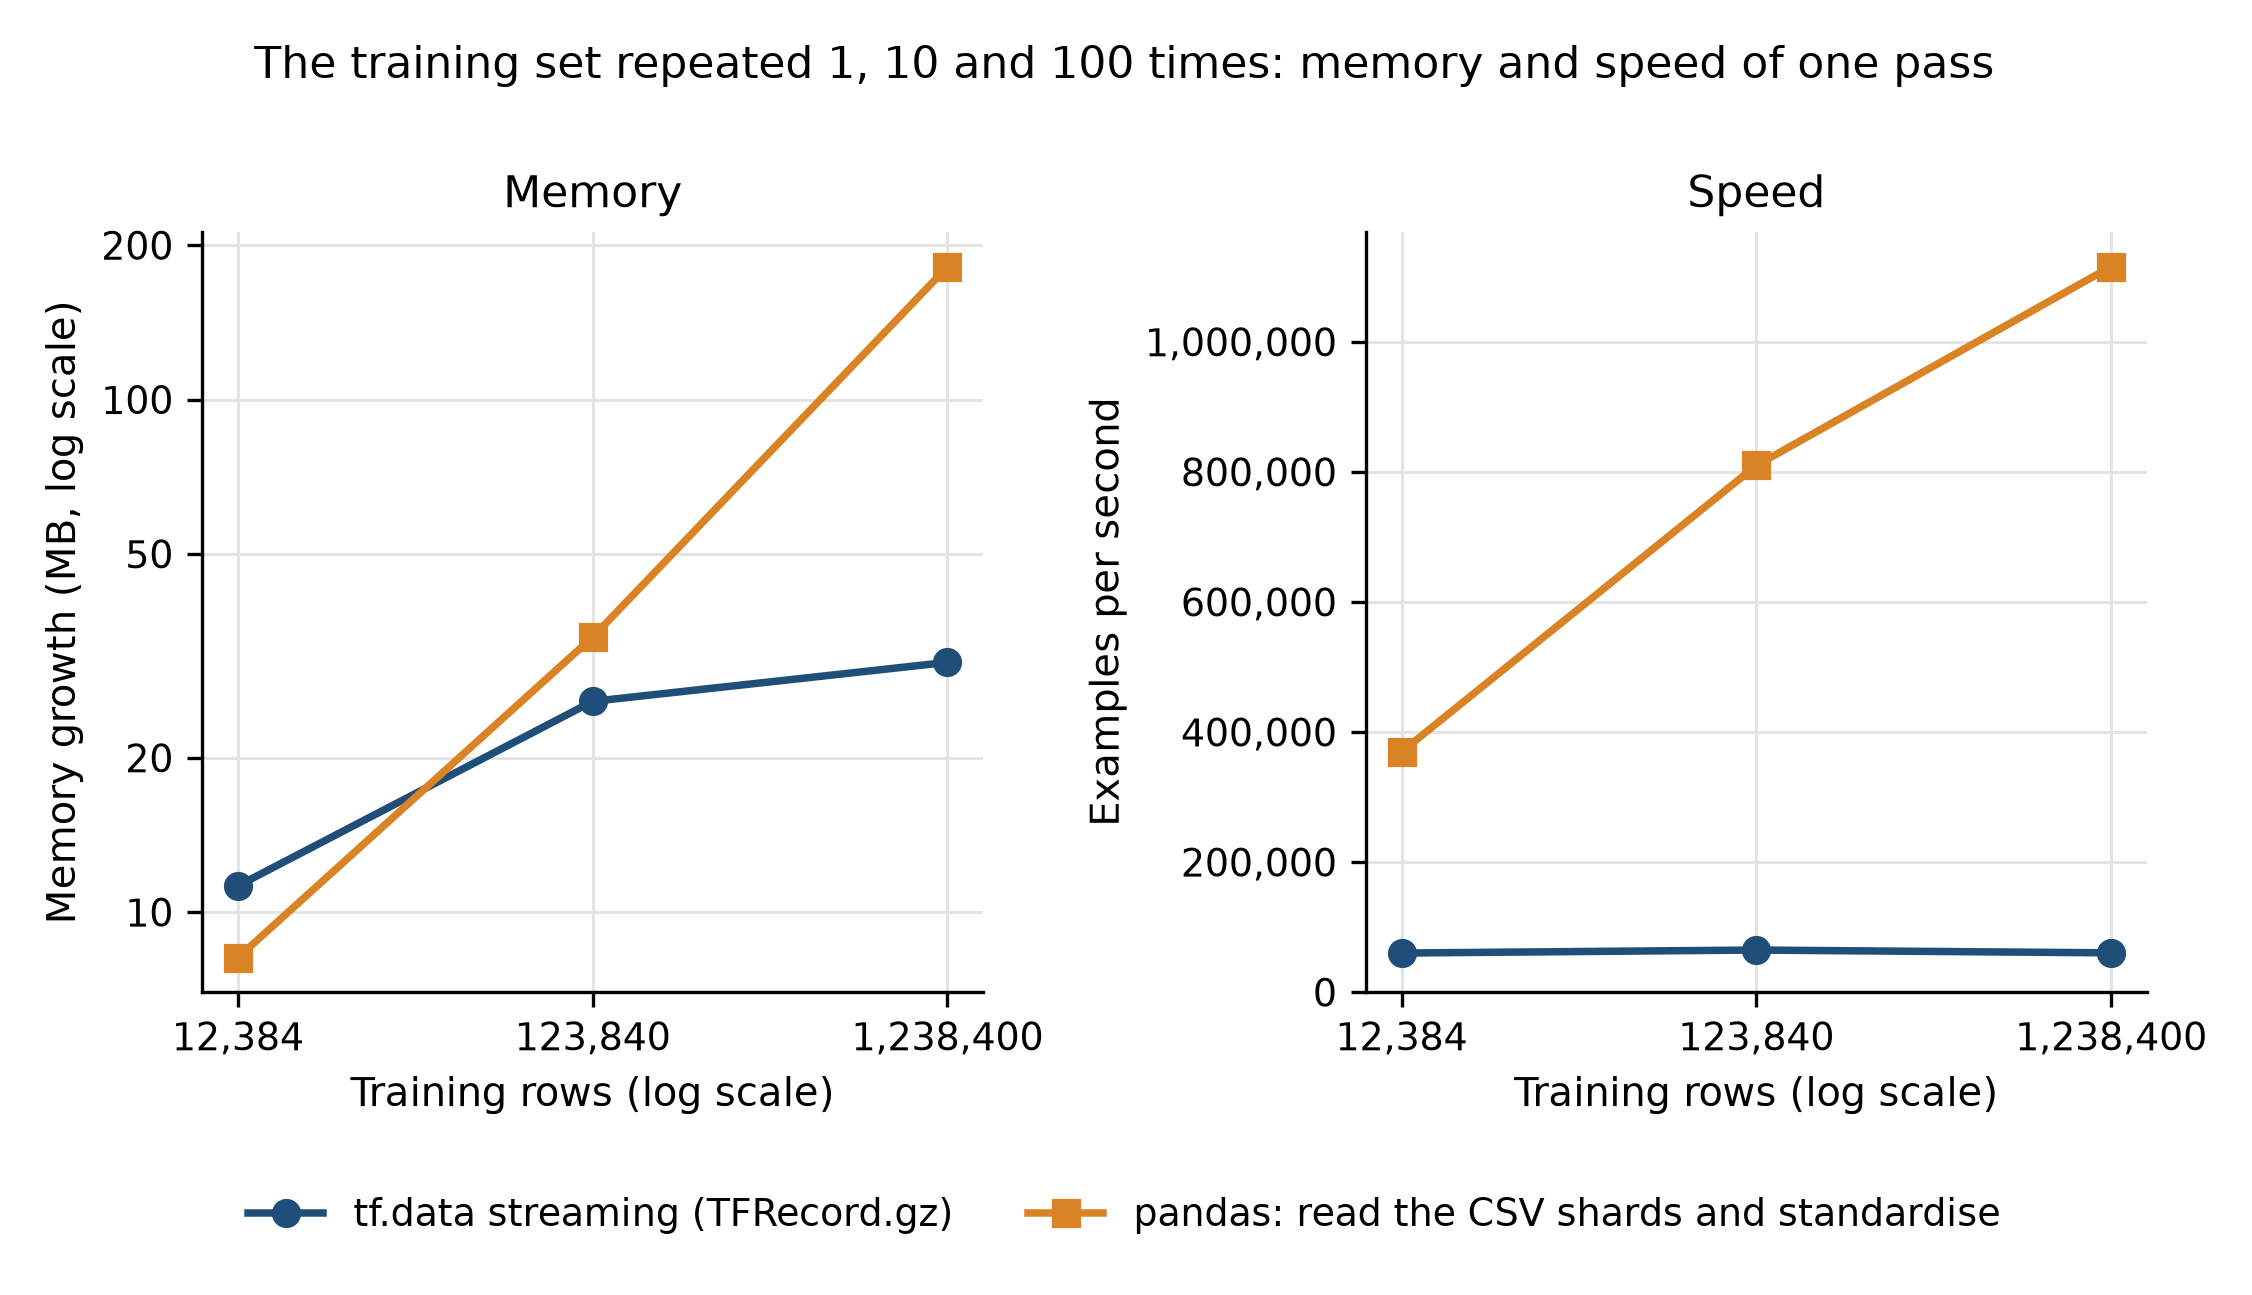
\includegraphics[width=\textwidth]{b_scale_test.png}
\caption{Memory growth (left) and reading speed (right) of the streaming pipeline and of pandas when the training set is repeated up to 100 times.}
\label{fig:scale}
\end{figure}

The memory of the streaming pipeline grows from \val{scale:growth:stream:min} to \val{scale:growth:stream:max}~MB, while the 100-fold data set grows by a factor of 100; that of pandas grows from \val{scale:growth:pandas:min} to \val{scale:growth:pandas:max}~MB, which is \val{scale:growth:ratio} times as much as the pipeline at the largest size, and it would keep growing with the data. The speed of the pipeline stays between \val{scale:speed:min} and \val{scale:speed:max} examples per second at every size. For the smallest data set the pipeline needs more memory than pandas; a plausible reason, which I did not test, is the fixed cost of the buffers and thread pools of \texttt{tf.data}. Two things must not be overlooked. Pandas is faster in time: loading the \val{scale:rows:max} rows takes \val{scale:pandas:max}~s, a pass of the streaming pipeline takes \val{scale:pass:max}~s, and the two do not do the same work, since the pipeline also shuffles, parses and batches. And the pandas data frame at the largest size still fits in memory comfortably, so these data do not yet show the case in which the streaming approach is the only one that works. They show how the two approaches scale: while the data grow by a factor of 100, the memory of the pipeline grows by a factor of \val{scale:ratio:stream} and that of pandas by a factor of \val{scale:ratio:pandas} (factors computed from the unrounded measurements, so they differ slightly from the ratios of the rounded cells of Table~\ref{tab:scale}).

\section{Part C: preprocessing inside the model}
\label{sec:features}

\subsection{From the Features API to Keras layers}

Chapter~13 builds the features of a model with \texttt{tf.feature\_column}: standardised numeric columns, a bucketised column, a categorical column with a vocabulary turned into an indicator (one-hot) column, a crossed column that is hashed, and an embedding column, all joined by a \texttt{DenseFeatures} layer. Keras~3 no longer contains \texttt{DenseFeatures}, so I built the same features with Keras preprocessing layers, which are part of the model (Table~\ref{tab:mapping}). The boundaries, the vocabulary, the 20 by 20 grid and the sizes of the hash tables (100 and 1,000 buckets) are the numbers of the book.

\begin{table}[!htbp]
\centering
\small
\begin{tabular}{L{7.5cm}L{7.1cm}}
\toprule
Book (\texttt{tf.feature\_column}) & This project (Keras 3 layers) \\
\midrule
\texttt{numeric\_column} with \texttt{normalizer\_fn} & \texttt{Normalization} with the training mean and variance \\
\texttt{bucketized\_column} & \texttt{Discretization} \\
\texttt{categorical\_column\_with\_\allowbreak vocabulary\_list} & \texttt{StringLookup}; index 0 is the bucket for unseen values \\
\texttt{indicator\_column} (one-hot) & the one-hot output mode of the lookup or the discretisation \\
\texttt{crossed\_column} (hashed) & \texttt{HashedCrossing} \\
\texttt{embedding\_column} & \texttt{Embedding} \\
\texttt{DenseFeatures} & \texttt{Concatenate} of the blocks \\
\bottomrule
\end{tabular}
\caption{The Features API of the book and the layers that replace it.}
\label{tab:mapping}
\end{table}

Because the layers are part of the model, the model takes the raw columns, and the preprocessing that is used in training is the one that is used when the model is served. The book's TF~Transform section warns about the difference between the two (training/serving skew); here a quality gate checks that the request path and the \texttt{tf.data} path give the same predictions (Section~\ref{sec:model}). The layers that have no learned weights are also tested against a plain NumPy computation of the same features on the validation rows; the largest difference is \metric{C}{layer_check_max_abs_diff}.

\subsection{The features}

Three ideas of the chapter are implemented.

\paragraph{One-hot encoding of a categorical column.} \texttt{ocean\_proximity} has five categories. A \texttt{StringLookup} layer with the five-word vocabulary turns it into a one-hot vector of six elements: the first element is the bucket for any category that the model has not seen, so that an unknown word at serving time gives an answer instead of an error.

\paragraph{A crossed grid of latitude and longitude.} Latitude is cut at 19 equally spaced boundaries from 32 to 42 degrees, which gives 20 intervals of which the first and the last are open-ended, longitude in the same way into 20 intervals with boundaries from $-125$ to $-114$ degrees, and the two are crossed into a grid of $20 \times 20 = 400$ cells. Two forms are used. The exact grid is the outer product of the two one-hot vectors, a one-hot vector of 400 elements. The book's form hashes the pair of indices into 1,000 buckets (with \texttt{HashedCrossing} here); the book says that the number of buckets must be high enough to avoid too many collisions and that a higher number needs more memory for the embedding table. With 400 cells in 1,000 buckets this form does not make the table smaller than the exact grid; I used it because it is the form of the book. Section~\ref{sec:math} computes how many collisions to expect when 400 cells are hashed into 1,000 buckets.

\paragraph{Embeddings.} An embedding replaces a one-hot vector by a short vector of learned numbers: of dimension 2 for the five categories, which is the value of the book, and of dimension 8 for the cells of the grid and 4 for the cross of age and category, which are choices of this project (age is cut into six intervals and crossed with \texttt{ocean\_proximity}, hashed into 100 buckets). The embedding of the exact 400 cells is implemented as a \texttt{Dense} layer without a bias on the one-hot vector, which is the same thing (Section~\ref{sec:math}); the embedding of the hashed cells is an \texttt{Embedding} layer. Section~\ref{sec:math} shows that an embedding is a one-hot vector multiplied by a matrix, and a test in the package checks that a dense layer without a bias on the one-hot input and an embedding give the same output.

\subsection{Feature sets and the experiment}

The nine feature sets of Table~\ref{tab:featuresets} are compared. Each set adds one idea to the baseline, the numbers plus the one-hot \texttt{ocean\_proximity}, except the first, which has the numbers only, and the last, which combines the income buckets, the age cross and the hashed grid. Each set is used in two models: a linear model, which has no hidden layer, so that the quality of the features is visible without a network that could construct features itself, and a small neural network with two hidden layers of 64 units. Every combination is trained with \metric{C}{n_seeds} seeds, with early stopping on the validation error, reading the GZIP-compressed TFRecord shards with \texttt{tf.data}. This makes \metric{C}{n_feature_sets} feature sets $\times$ 2 models $\times$ \metric{C}{n_seeds} seeds trainings. The comparison uses the validation set; the test error is shown for information and is not used to choose.

\begin{table}[!htbp]
\centering
\small
\begin{tabular}{llp{8.6cm}}
\toprule
 & Feature set & Inputs of the model \\
\midrule
1 & numeric only & the 8 standardised numbers \\
2 & + ocean one-hot & 1, and the one-hot vector of \texttt{ocean\_proximity} (baseline) \\
3 & + ocean embedding & 1, and a 2-dimensional embedding of \texttt{ocean\_proximity} \\
4 & + income buckets & 2, and the one-hot vector of the income bucket (boundaries 1.5, 3, 4.5 and 6) \\
5 & + age $\times$ ocean & 2, and a 4-dimensional embedding of the hashed cross of age and ocean (100 buckets) \\
6 & + grid one-hot (400) & 2, and the one-hot vector of the 400 grid cells \\
7 & + grid embedding (400) & 2, and an 8-dimensional embedding of the 400 grid cells \\
8 & + hashed grid (1000) & 2, and an 8-dimensional embedding of the 400 cells hashed into 1,000 buckets \\
9 & all features & 2, the income buckets, the age cross and the hashed grid \\
\bottomrule
\end{tabular}
\caption{The nine feature sets.}
\label{tab:featuresets}
\end{table}

Differences between feature sets are tested with paired seeds (Section~\ref{sec:math}): for each seed the two sets use the same seed for the shuffling of the data and for the initialisation, so the difference of their errors removes part of the noise of training. A difference is called clear when the 95\% interval of the mean difference does not contain 0.

\subsection{Results}

Tables~\ref{tab:featlin} and~\ref{tab:featmlp} give, for each feature set, the mean validation RMSE over the \metric{C}{n_seeds} seeds, the paired difference from the baseline with its 95\% interval, and the test RMSE; Figure~\ref{fig:ablation} shows the test RMSE with its interval across seeds.

\begin{table}[!htbp]
\centering
\footnotesize
\setlength{\tabcolsep}{4pt}
\begin{tabular}{L{3.9cm}R{1.0cm}R{1.2cm}R{1.3cm}L{4.0cm}R{1.3cm}R{1.0cm}}
\toprule
Feature set & Inputs & Params & Valid. RMSE & Diff. from baseline\newline [95\% interval] & Test RMSE & Test $R^2$ \\
\midrule
numeric only & 8 & 9 & 69,626 & $+$770 [$+$746, $+$793]* & 68,473 & 0.640 \\
+ ocean one-hot & 14 & 15 & 68,856 & baseline & 67,490 & 0.651 \\
+ ocean embedding & 10 & 23 & 68,902 & $+$46 [$+$2, $+$89]* & 67,462 & 0.651 \\
+ income buckets & 19 & 20 & 67,980 & $-$876 [$-$901, $-$850]* & 66,604 & 0.660 \\
+ age $\times$ ocean & 18 & 419 & 68,580 & $-$276 [$-$309, $-$243]* & 67,149 & 0.654 \\
+ grid one-hot (400) & 414 & 415 & 64,226 & $-$4,630 [$-$4,657, $-$4,602]* & 62,546 & 0.700 \\
+ grid embedding (400) & 22 & 3,223 & 64,583 & $-$4,273 [$-$4,371, $-$4,174]* & 62,787 & 0.698 \\
+ hashed grid (1000) & 22 & 8,023 & 64,675 & $-$4,182 [$-$4,352, $-$4,011]* & 62,846 & 0.697 \\
all features & 31 & 8,432 & 63,211 & $-$5,645 [$-$5,737, $-$5,553]* & 61,316 & 0.712 \\
\bottomrule
\end{tabular}

\caption{Linear model on each feature set. Errors in dollars. The baseline is \texttt{+ ocean one-hot}; a negative difference is an improvement, and * marks an interval that excludes 0.}
\label{tab:featlin}
\end{table}

\begin{table}[!htbp]
\centering
\footnotesize
\setlength{\tabcolsep}{4pt}
\begin{tabular}{L{3.9cm}R{1.0cm}R{1.2cm}R{1.3cm}L{4.0cm}R{1.3cm}R{1.0cm}}
\toprule
Feature set & Inputs & Params & Valid. RMSE & Diff. from baseline\newline [95\% interval] & Test RMSE & Test $R^2$ \\
\midrule
numeric only & 8 & 4,801 & 52,303 & $-$312 [$-$1,088, $+$464] & 51,852 & 0.794 \\
+ ocean one-hot & 14 & 5,185 & 52,616 & baseline & 51,530 & 0.796 \\
+ ocean embedding & 10 & 4,941 & 52,180 & $-$436 [$-$1,159, $+$287] & 51,387 & 0.797 \\
+ income buckets & 19 & 5,505 & 53,079 & $+$463 [$-$133, $+$1,059] & 51,730 & 0.795 \\
+ age $\times$ ocean & 18 & 5,841 & 52,706 & $+$90 [$-$488, $+$669] & 51,814 & 0.794 \\
+ grid one-hot (400) & 414 & 30,785 & 52,759 & $+$143 [$-$356, $+$642] & 51,590 & 0.796 \\
+ grid embedding (400) & 22 & 8,897 & 52,230 & $-$385 [$-$964, $+$193] & 51,065 & 0.800 \\
+ hashed grid (1000) & 22 & 13,697 & 52,002 & $-$614 [$-$1,191, $-$36]* & 50,668 & 0.803 \\
all features & 31 & 14,673 & 52,803 & $+$188 [$-$586, $+$961] & 51,606 & 0.796 \\
\bottomrule
\end{tabular}

\caption{Neural network with two hidden layers of 64 units on each feature set, in the same form as Table~\ref{tab:featlin}.}
\label{tab:featmlp}
\end{table}

\begin{figure}[!htbp]
\centering
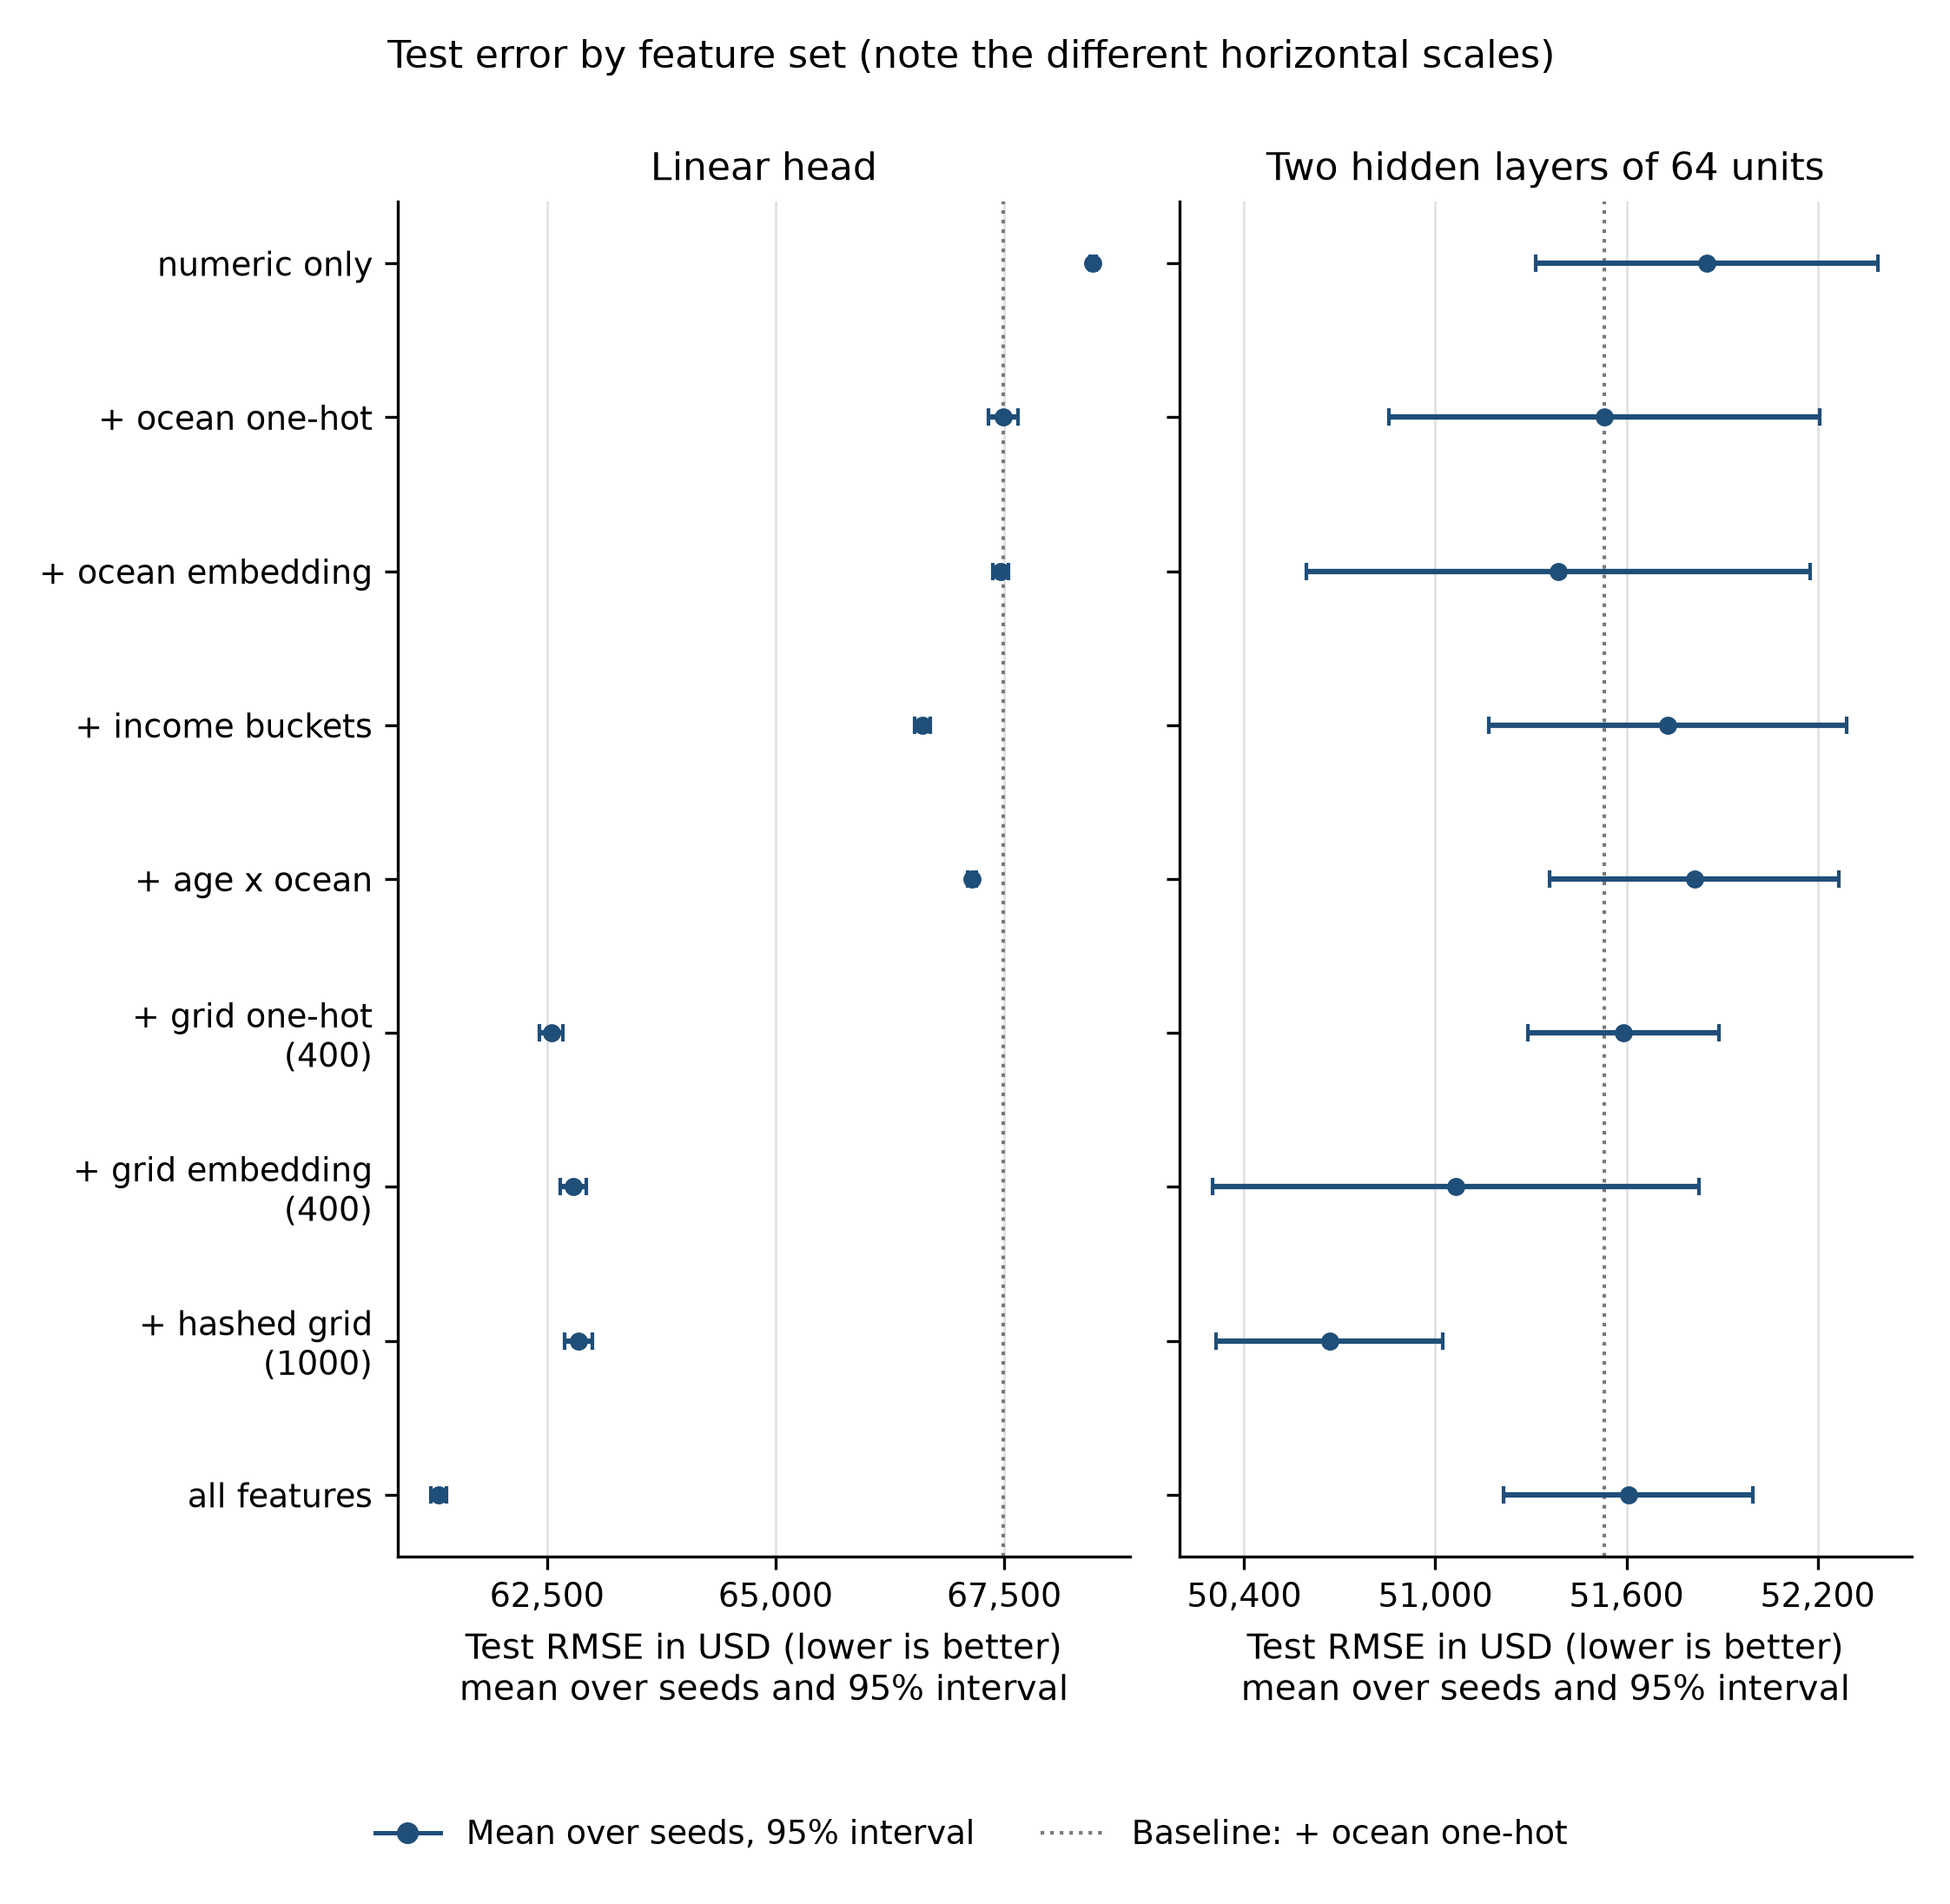
\includegraphics[width=\textwidth]{c_feature_ablation.png}
\caption{Test RMSE of the nine feature sets for the linear model (left) and the neural network (right): mean over the seeds with the 95\% interval.}
\label{fig:ablation}
\end{figure}

\paragraph{Linear model.} The features matter for the linear model. The baseline has a validation RMSE of \$\val{c:linear:base}. Crossing latitude and longitude into the exact grid of 400 cells lowers it by \$\val{c:linear:grid-one-hot-400:diff} (\val{c:linear:grid-one-hot-400:pct}\%), and the two grid forms that use 22 inputs instead of 414, the learned embedding of the 400 cells and the hashed grid, lower it by \$\val{c:linear:grid-embedding-400:diff} and \$\val{c:linear:hashed-grid-1000:diff}. A linear model can make the price depend on the position only linearly in latitude and longitude; the grid gives every cell its own coefficient. All features together lower the error by \$\val{c:linear:all-features:diff} (\val{c:linear:all-features:pct}\%). The income buckets (\$\val{c:linear:income-buckets:diff}) and the cross of age and category (\$\val{c:linear:age-x-ocean:diff}) help little; the one-hot category itself is worth \$\val{c:linear:numeric-only:diff} against the numbers alone, and a 2-dimensional embedding of the category is almost as good as the one-hot vector (\$\val{c:linear:ocean-embedding:diff} worse). For all \val{c:linear:ncompared} comparisons the interval excludes 0, but the intervals are very narrow, because a linear model trained with different seeds ends almost in the same place. They describe the variation caused by the seeds and not what another split of the data would change.

\paragraph{Neural network.} With two hidden layers the baseline is already \val{c:mlp:over:linear:pct}\% better than the linear model (a validation RMSE of \$\val{c:mlp:base}), and the additional features change little. Only one of the \val{c:mlp:ncompared} comparisons has an interval that excludes 0: the hashed grid improves the validation RMSE by \$\val{c:mlp:hashed-grid-1000:diff} (\val{c:mlp:hashed-grid-1000:pct}\%), with an interval from $-$\$\val{c:mlp:hashed-grid-1000:difflo} to $-$\$\val{c:mlp:hashed-grid-1000:diffhi}. All features together are not better than the baseline (a difference of $+$\$\val{c:mlp:all-features:diff}, with an interval that contains 0). A plausible explanation, which I did not test separately, is that the hidden layers can build functions of position from raw latitude and longitude themselves, so that the grid adds less than it does for the linear model. The result of the single interval should be read with care (this is my own reading, not the book's): eight intervals of 95\% were computed for this model, and one that only just excludes 0 is not strong evidence. The set with the lowest mean validation error of the neural network, \texttt{\val{c:mlp:best:name}}, is the one that is deployed (Section~\ref{sec:model}); the rule uses the validation set and not the test set. Compared in the same paired way with the network on the eight numbers alone, the number of the \val{c:mlp:vsnum:n} richer feature sets whose interval shows them to be better is \val{c:mlp:vsnum:nbetter}. Replacing the one-hot grid of 400 cells by an 8-dimensional embedding lowers the mean error from \$\val{c:mlp:grid-one-hot-400:valid} to \$\val{c:mlp:grid-embedding-400:valid} and reduces the parameters from \val{c:mlp:grid-one-hot-400:params} to \val{c:mlp:grid-embedding-400:params}; the paired interval of this difference is from \val{pair:mlp:gridemb:lo} to \val{pair:mlp:gridemb:hi}, so on these data the smaller form was not worse. The paired comparisons of this paragraph and the next were chosen after looking at the tables, so the caveat about many intervals applies to them as well.

\paragraph{Hash collisions of the location cross.} The 400 cells land in \metric{C}{hash_distinct_buckets_all_cells} distinct buckets out of 1,000, so \val{hash:shared:cells} cells share a bucket with a cell that was there first. A uniformly random hash would be expected to use \val{hash:expected} buckets and to cause \val{hash:expected:shared} such sharings (Table~\ref{tab:hash}, Figure~\ref{fig:grid}). Only \metric{C}{hash_cells_with_training_rows} of the 400 cells contain training rows, since the data cover only a part of the rectangle that the grid spans, and of these just \metric{C}{hash_occupied_cells_sharing_a_bucket} share a bucket with another occupied cell; the training rows in these buckets are \val{hash:rows:pct}\% of the data. In this project the same cells collided in repeated calls; I did not check other versions of Keras. The collisions were not isolated in a separate experiment, so I do not claim that they are harmless. For the neural network the hashed grid has the lower mean error (\$\val{c:mlp:hashed-grid-1000:valid} against \$\val{c:mlp:grid-one-hot-400:valid} for the exact grid, a paired interval of the difference from \val{pair:mlp:hash:lo} to \val{pair:mlp:hash:hi}). For the linear model it is \$\val{hash:lin:worse} worse (\$\val{c:linear:hashed-grid-1000:valid} against \$\val{c:linear:grid-one-hot-400:valid}, a paired interval from \val{pair:lin:hash:lo} to \val{pair:lin:hash:hi}), and its mean is \$\val{hash:lin:worse:emb} above that of the embedding of the exact cells, a difference whose paired interval, from \val{pair:lin:hashemb:lo} to \val{pair:lin:hashemb:hi}, contains 0.

\begin{table}[!htbp]
\centering
\small
\begin{tabular}{p{10cm}r}
\toprule
Quantity & Value \\
\midrule
Grid cells & 400 \\
Hash buckets & 1,000 \\
Distinct buckets used by all cells (measured) & 335 \\
Distinct buckets expected for a uniform random hash & 329.8 \\
Cells that contain training rows & 133 \\
Occupied cells that share a bucket with another occupied cell & 6 \\
Training rows in such shared buckets & 94 (0.76\%) \\
\bottomrule
\end{tabular}

\caption{Hashing the 400 grid cells into 1,000 buckets.}
\label{tab:hash}
\end{table}

\begin{figure}[!htbp]
\centering
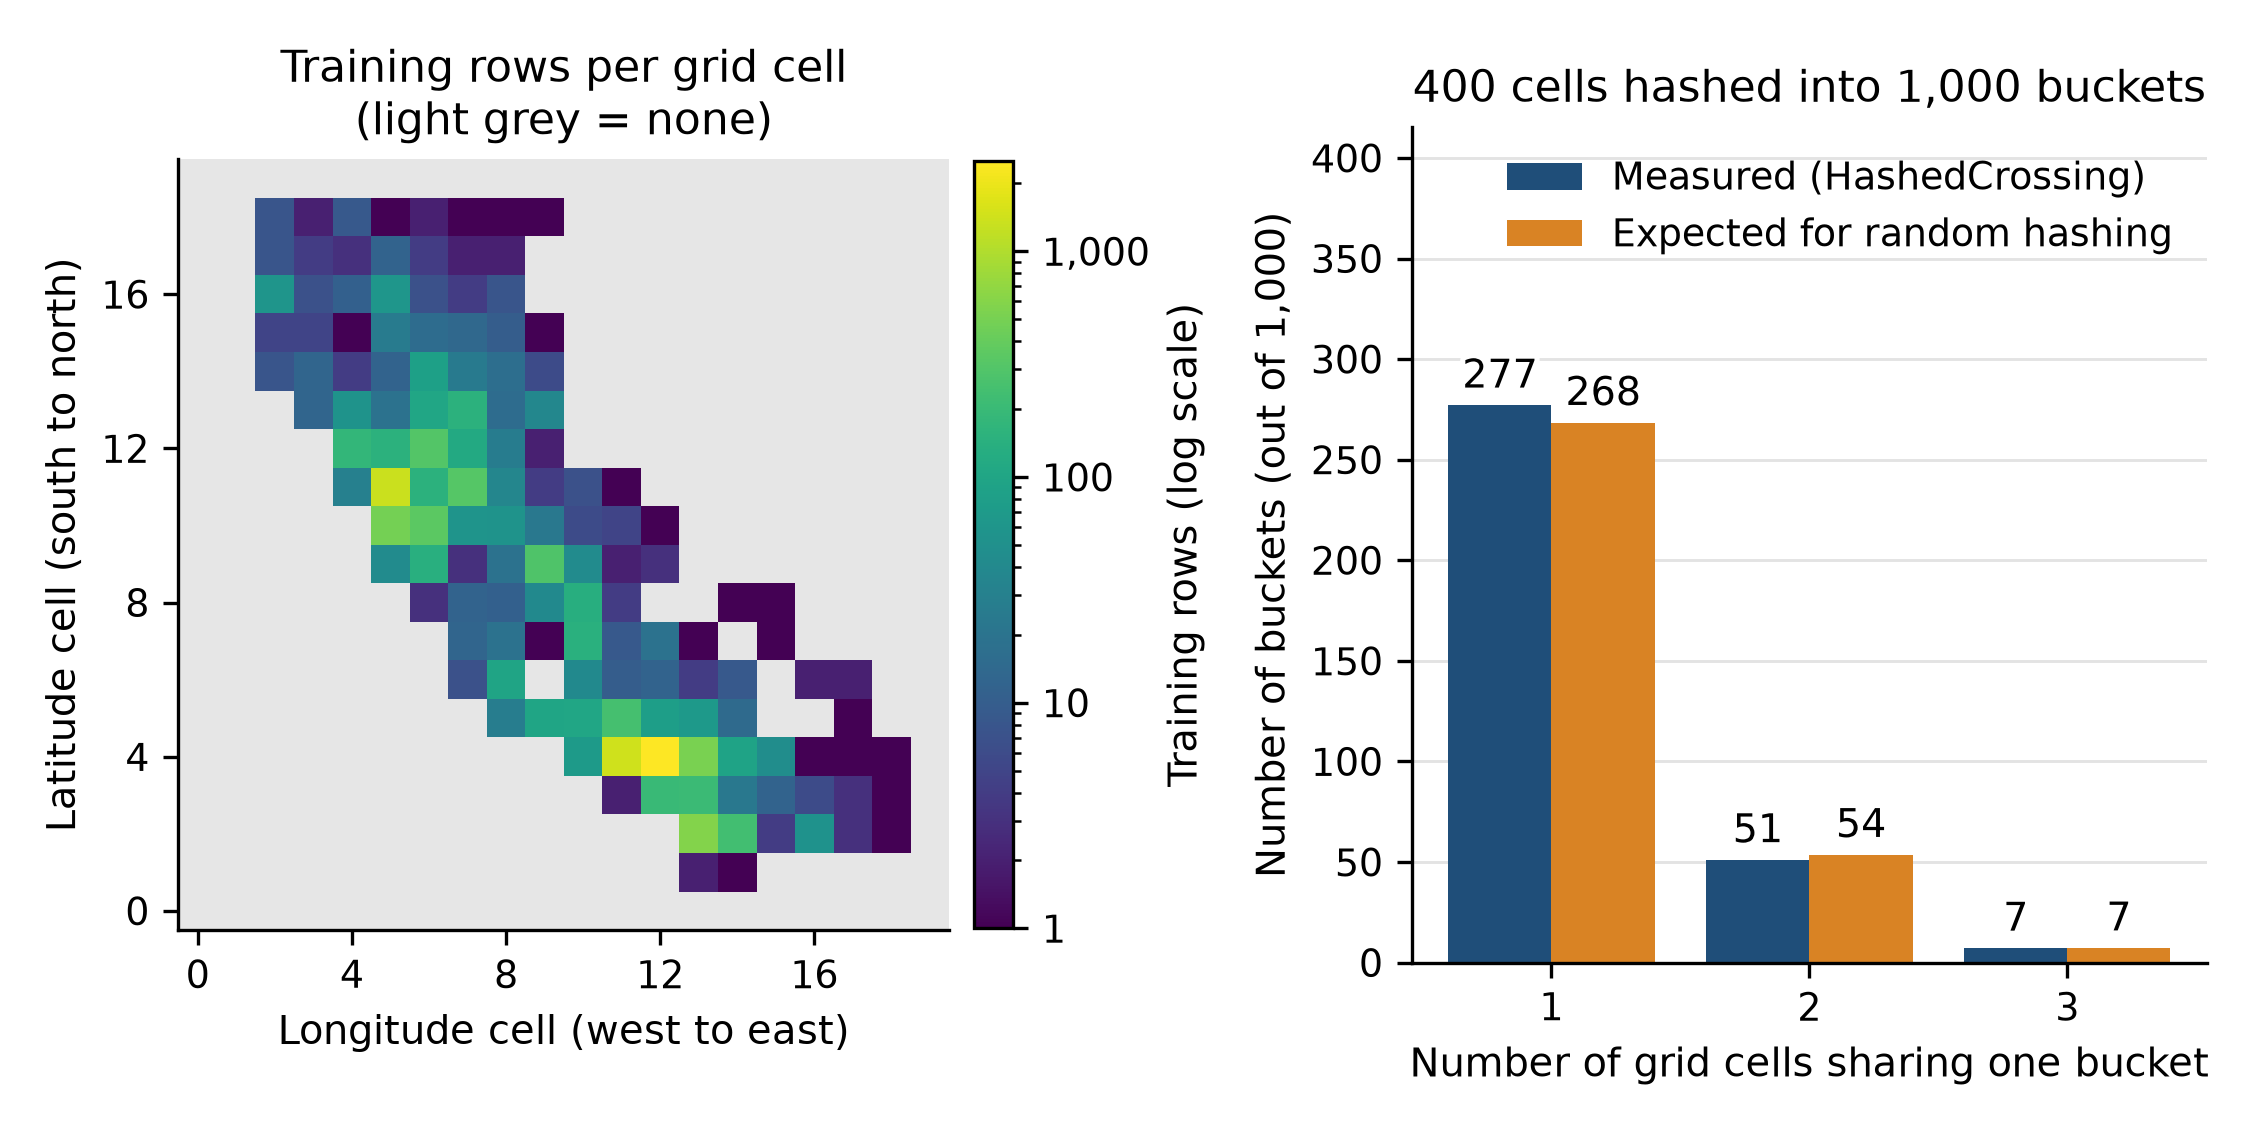
\includegraphics[width=\textwidth]{c_location_grid.png}
\caption{Left: the number of training rows in each cell of the 20 by 20 grid (light grey: none). Right: the number of buckets that hold $k$ cells, measured and expected for a uniform random hash.}
\label{fig:grid}
\end{figure}

\section{Part D: TensorFlow Datasets and images in TFRecord files}
\label{sec:tfds}

\subsection{\texttt{tfds.load}}

The last section of Chapter~13 loads MNIST and trains on it with a few lines (the model definition is elided in the book, as is its \texttt{compile} call):

\begin{verbatim}
dataset = tfds.load(name="mnist", batch_size=32, as_supervised=True)
mnist_train = dataset["train"].repeat().prefetch(1)
model.fit(mnist_train, steps_per_epoch=60000 // 32, epochs=5)
\end{verbatim}

The project makes the first call with the same arguments. The result is a dictionary with a \texttt{train} and a \texttt{test} data set, each already batched, whose elements are a batch of images (28 by 28 pixels, one channel, unsigned bytes) and a batch of labels. The training set has \metric{D}{train_batches} batches of 32 images, the number that the book's \texttt{steps\_per\_epoch} gives for \metric{D}{n_train_images} images, and the test set has \metric{D}{test_batches} batches, the last of which is not full because 10,000 is not a multiple of 32.

The version of TFDS used here downloads the four official MNIST files from a Google Cloud Storage address. Some firewalls and CI runners cannot reach that address, and this project was built in such an environment, so the project can fetch the same four files from a public mirror, compare their MD5 checksums with the official ones and hand them to the MNIST builder of TFDS; everything after the download is then the real \texttt{tfds.load} (Section~\ref{sec:limits}). The route of this run was \texttt{\param{D}{source}}.

\subsection{MNIST stored as TFRecord files}

The book explains that a \texttt{BytesList} can hold any binary data: an image encoded with \texttt{tf.io.encode\_jpeg}, or any tensor turned into a byte string with \texttt{tf.io.serialize\_tensor}. Three encodings of the \metric{D}{n_train_images} training images are compared, each in \param{D}{n_shards} shards, once uncompressed and once with GZIP. The first is the serialised tensor of the book. The second is an encoded image; it is PNG and not the book's JPEG, because PNG is lossless and the pixels that come back can be compared with the original ones. The third, the plain bytes of the pixel array, is an addition of this project (it is not in the book) and the only one that can be decoded for a whole batch at a time, because in the code of this project \texttt{tf.io.decode\_raw} accepts a vector of strings, while \texttt{tf.io.decode\_png} and \texttt{tf.io.parse\_tensor} take one string. For all three encodings, the first 256 training images and their labels come back from the files exactly equal to the originals.

\begin{table}[!htbp]
\centering
\small
\setlength{\tabcolsep}{5pt}
\begin{tabular}{llR{2.1cm}R{1.6cm}R{1.6cm}R{1.6cm}R{1.6cm}}
\toprule
 & & & \multicolumn{2}{c}{One record at a time} & \multicolumn{2}{c}{A batch at a time} \\
\cmidrule(lr){4-5}\cmidrule(lr){6-7}
Encoding & Compression & Bytes/image & Serial & Parallel & Serial & Parallel \\
\midrule
raw & none & 838 & 23,461 & 20,452 & 121,449 & 64,376 \\
raw & GZIP & 173 & 26,791 & 20,369 & 89,173 & 56,684 \\
png & none & 331 & 23,474 & 19,083 & -- & -- \\
png & GZIP & 242 & 22,866 & 16,655 & -- & -- \\
tensor & none & 857 & 27,490 & 21,543 & -- & -- \\
tensor & GZIP & 173 & 25,460 & 18,205 & -- & -- \\
\bottomrule
\end{tabular}

\caption{Size and reading speed of the MNIST training images in three encodings. Speeds are in images per second, with no training step. ``Parallel'' uses \texttt{tf.data.AUTOTUNE} for reading, decoding and prefetching, ``serial'' uses none of these. A dash marks a combination that does not exist for that encoding.}
\label{tab:mnistformats}
\end{table}

\begin{figure}[!htbp]
\centering
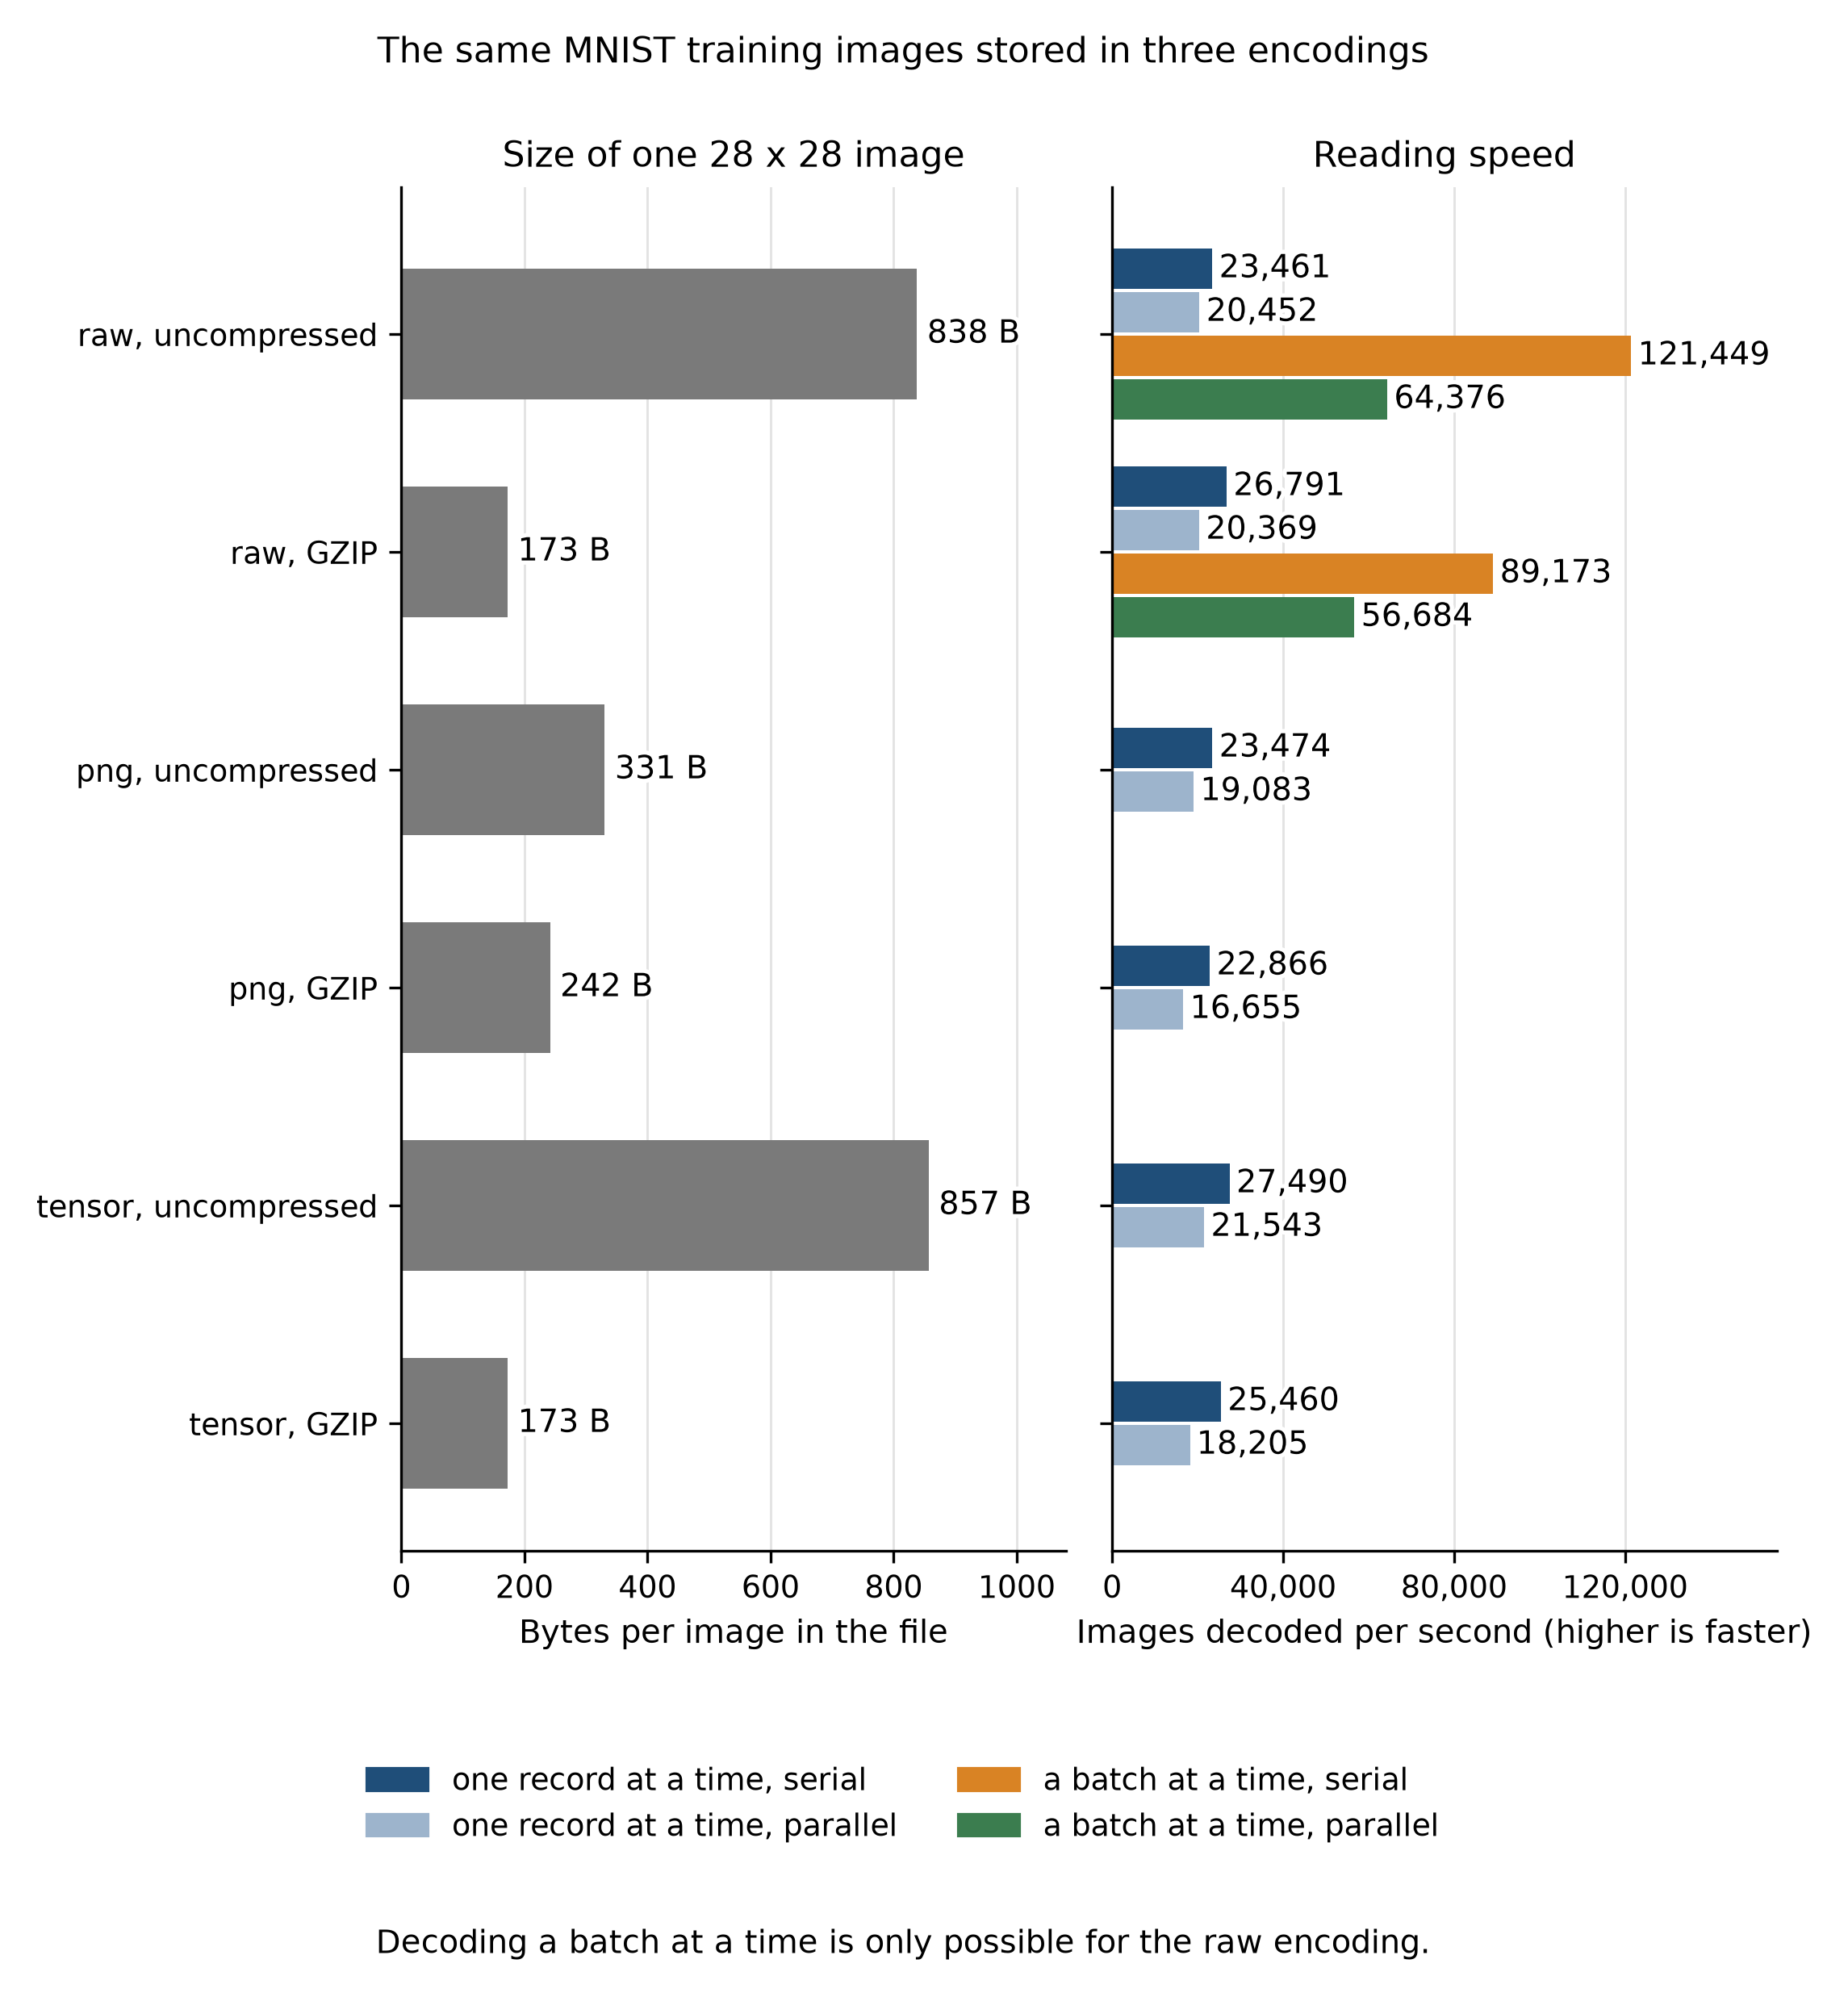
\includegraphics[width=\textwidth]{d_mnist_formats.png}
\caption{Size per image (left) and reading speed (right) of the six files of Table~\ref{tab:mnistformats}.}
\label{fig:mnist}
\end{figure}

\paragraph{Size.} The sizes are in Table~\ref{tab:mnistformats} and Figure~\ref{fig:mnist}; the factors below are computed from the unrounded sizes. A raw record takes \val{mnist:raw} bytes for \val{mnist:pixels} pixels. The \val{mnist:raw:overhead} bytes in addition are the 16 bytes of framing of the record (Section~\ref{sec:math}) and the \texttt{Example} structure with the names \texttt{image} and \texttt{label}. The serialised tensor takes \val{mnist:tensor:extra} bytes more than the raw bytes (\val{mnist:tensor} bytes), which is the description of type and shape that it carries. A PNG image is \val{mnist:png:over:raw} times as large as the raw bytes (\val{mnist:png} bytes), because PNG compresses a picture that is mostly black. GZIP shrinks the raw and the tensor records to \val{mnist:raw:gz} and \val{mnist:tensor:gz} bytes, factors of \val{mnist:raw:gz:ratio} and \val{mnist:tensor:gz:ratio}, and the PNG records to \val{mnist:png:gz} bytes. The compressed raw record is therefore smaller than the PNG record, with or without GZIP on top of PNG. A plausible reason, which I did not test, is that GZIP is applied to the whole stream of records and can use what repeats from one record to the next, whereas PNG compresses one image at a time.

\paragraph{Speed.} Decoding one record at a time in serial, the six files are read at between \val{mnist:single:min} and \val{mnist:single:max} images per second, which is a spread of \val{mnist:single:spread}\%. Each configuration was timed in one experiment, and in Part~A the same CSV pipeline timed in two experiments of one run differed by \val{noise:pct}\% (Section~\ref{sec:csv}); I therefore do not draw a conclusion about which of the single-record encodings decodes fastest. The result that is large enough to be an effect is the one of Part~B: decoding a whole batch of raw records in one call reads \val{mnist:batch:plain} images per second from the uncompressed files and \val{mnist:batch:gz} from the compressed ones, which is \val{mnist:batch:over:single:plain} and \val{mnist:batch:over:single:gz} times as fast as one record at a time (for the housing rows the factor was \val{fmt:batch:over:single}). As in Part~B, the comparison mixes the effect of batching with that of the encoding, because the other two encodings could not be decoded for a batch at once. The \texttt{AUTOTUNE} variants were slower than their serial counterparts in all \val{mnist:par:n} cases, by factors between \val{mnist:par:over:ser:min} and \val{mnist:par:over:ser:max}, in line with what Part~A found for \texttt{AUTOTUNE} on this two-core machine; I did not investigate the cause.

\subsection{The same classifier from both sources}

A small classifier is trained from the two sources: the batches of \texttt{tfds.load}, used as in the book, and the compressed raw TFRecord files read with a shuffle buffer of 10,000 images and batch-wise decoding. The book elides the layers of its model and uses the optimiser \texttt{sgd}; the classifier here is a choice of the project (the pixels divided by 255, one hidden layer of 128 units, a softmax layer of 10 units, Adam), so its accuracy is not comparable with any number of the book. Both are trained for \param{D}{epochs} epochs of 1,875 batches with the same \metric{D}{n_train_images} training images and with \param{D}{n_seeds} seeds, the two sources sharing the random numbers of the initialisation for each seed. The accuracy is that on the test set after the last epoch; nothing was chosen with it.

\begin{table}[!htbp]
\centering
\small
\begin{tabular}{lrrr}
\toprule
Input & Seeds & Mean test accuracy & Standard deviation \\
\midrule
\texttt{tfds.load} & 3 & 0.9757 & 0.0010 \\
TFRecord (raw, GZIP) & 3 & 0.9764 & 0.0010 \\
\bottomrule
\end{tabular}

\caption{Test accuracy of the same classifier trained from the two sources: mean and standard deviation over the seeds.}
\label{tab:mnistfits}
\end{table}

The mean accuracies (Table~\ref{tab:mnistfits}) are \val{mnist:acc:tfds} from \texttt{tfds.load} and \val{mnist:acc:tfrecord} from the TFRecord files, and all \val{mnist:acc:n}~$\times$~2 values lie between \val{mnist:acc:min} and \val{mnist:acc:max}. The paired difference (\texttt{tfds.load} minus TFRecord) has a mean of \val{mnist:acc:diff:mean} and a 95\% interval from \val{mnist:acc:diff:lo} to \val{mnist:acc:diff:hi}, which contains 0. With three seeds the interval is wide, so this shows that no difference was detected and not that there is none. It is a check that the TFRecord files lead to the same classifier as the data of TFDS; the exact comparison of the first 256 images (0.4\% of the 60,000) is direct evidence for those images only.

\section{Part E: the deployed model}
\label{sec:model}

\subsection{The model}

The model that is deployed is the neural network with two hidden layers of 64 units on the feature set \texttt{\param{E}{feature_set}}. It takes the raw columns, so its preprocessing layers (the standardisation, the buckets, the hashed cross and the embeddings of Section~\ref{sec:features}) are stored in the same file as its weights. It is trained on the GZIP-compressed TFRecord shards with early stopping on the validation error: it ran for \metric{E}{epochs_run} epochs, the best one being epoch \metric{E}{best_epoch}, and has \metric{E}{n_params} parameters. The validation RMSE is \$\metric{E}{valid_rmse}; this is the run with seed \param{E}{seed} of Part~C (the same seed and the same data give the same result), whereas the \$\val{c:mlp:hashed-grid-1000:valid} of Table~\ref{tab:featmlp} is the mean of \metric{C}{n_seeds} runs, and the two differ by the variation between seeds.

The choice of the feature set is not itself a finding. With the caveat about many intervals of Section~\ref{sec:features}, the comparisons do not show any feature set to be better for the network than the eight numbers alone: the mean validation errors of the nine sets lie between \$\val{c:mlp:valid:min} and \$\val{c:mlp:valid:max}, and the network on the numbers alone, with \val{c:mlp:numeric-only:params} parameters, is \$\val{pair:mlp:num:diff} behind the deployed set, with a paired interval from \val{pair:mlp:num:lo} to \val{pair:mlp:num:hi}. The deployed set was chosen by the stated rule, the lowest mean validation RMSE, so its small advantage should not be read as an effect.

\subsection{Quality on the test set}

The test set was not used to choose the model, the feature set or any setting of the training; the thresholds of the quality gates were set after a first run (Section~\ref{sec:limits}). Two yardsticks are used: always predicting the mean of the training targets, and the model of Chapter~2 of the book without its three combined attributes (median imputation, standardised numbers, one-hot category, linear regression) fitted on the same training rows.

\begin{table}[!htbp]
\centering
\small
\begin{tabular}{lrr}
\toprule
 & Test RMSE (USD) & 95\% interval (USD) \\
\midrule
Always the training mean & \metric{E}{baseline_mean_test_rmse} & \\
Linear model of Chapter 2 & \metric{E}{baseline_linear_test_rmse} & \\
Deployed model & \metric{E}{test_rmse} & \val{e:rmse:lo} to \val{e:rmse:hi} \\
\bottomrule
\end{tabular}
\caption{Error of the deployed model and of two yardsticks on the \runSplitNTest{} test rows. The interval is computed for the deployed model, whose predictions are stored with the results, by the method of Chapter~2 (Section~\ref{sec:math-paired}).}
\label{tab:final}
\end{table}

The deployed model has a test $R^2$ of \metric{E}{test_r2} and a mean absolute error of \$\metric{E}{test_mae}. Its test RMSE is \val{e:gain:linear:pct}\% lower than that of the linear model of Chapter~2 and \val{e:gain:mean:pct}\% lower than that of the mean. As in Chapter~2 of the book, a 95\% confidence interval for this error is computed from the squared errors of the test rows; it runs from \$\val{e:rmse:lo} to \$\val{e:rmse:hi}. It describes only the sampling variation of the \val{e:ntest} test rows: the model, its seed and the split are held fixed.

Chapter~2 of the book notes that the median house values were capped (Section~\ref{sec:data}). On the \val{cap:n} test rows at the largest value, \$\val{cap:value}, the RMSE of the deployed model is \$\val{cap:rmse} and its mean error is \val{cap:mean:err}; on the other \val{cap:rest:n} rows the RMSE is \$\val{cap:rest:rmse}.

Figure~\ref{fig:model} shows the learning curve, the predictions against the actual values, and the error by area type and by income band; the two tables behind the last panels are Tables~\ref{tab:errocean} and~\ref{tab:errincome}.

\begin{figure}[!htbp]
\centering
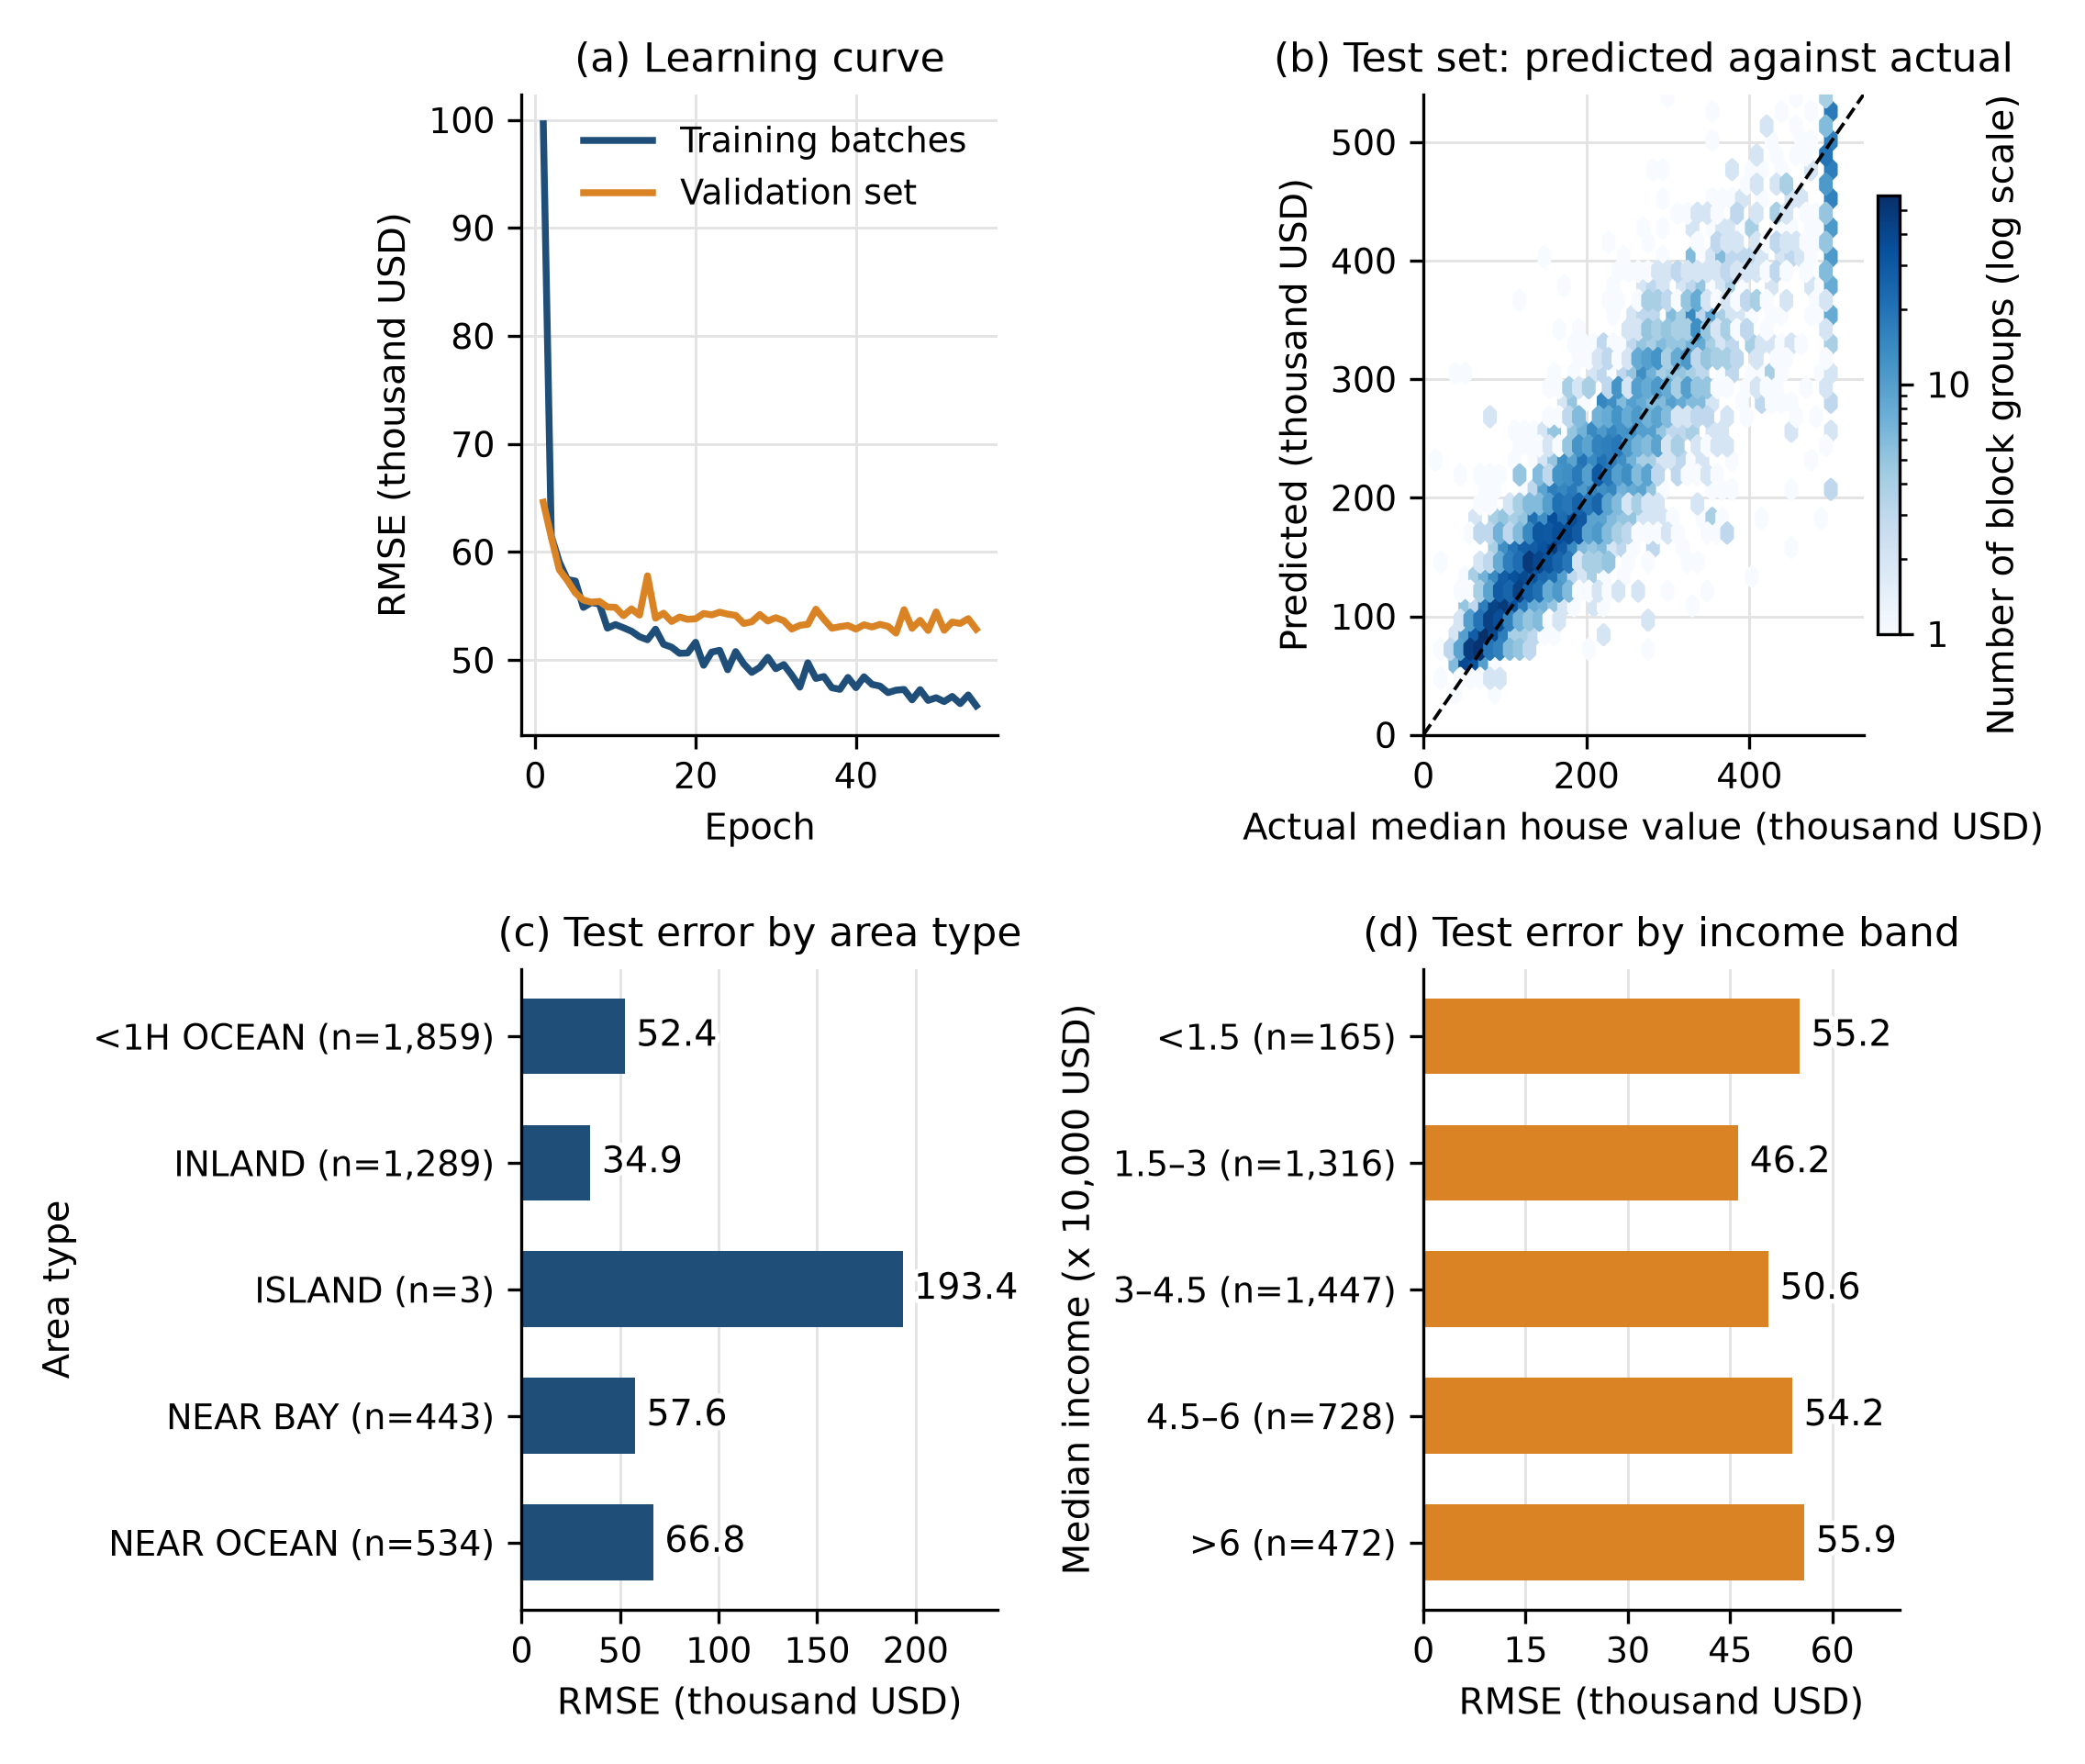
\includegraphics[width=\textwidth]{e_model_quality.png}
\caption{The deployed model. (a) RMSE on the training and validation data during training. (b) Predicted against actual value on the test set; the dashed line is a perfect prediction. (c), (d) RMSE on the test set by \texttt{ocean\_proximity} and by income band.}
\label{fig:model}
\end{figure}

\begin{table}[!htbp]
\centering
\small
\begin{tabular}{lrrr}
\toprule
Group & Test rows & RMSE (USD) & Mean error (USD) \\
\midrule
<1H OCEAN & 1,859 & 52,387 & $+$2,116 \\
INLAND & 1,289 & 34,881 & $+$3,807 \\
ISLAND & 3 & 193,405 & $+$2,647 \\
NEAR BAY & 443 & 57,556 & $-$130 \\
NEAR OCEAN & 534 & 66,795 & $+$4,043 \\
\bottomrule
\end{tabular}

\caption{Test error by \texttt{ocean\_proximity}. The mean error is the mean of prediction minus actual value.}
\label{tab:errocean}
\end{table}

\begin{table}[!htbp]
\centering
\small
\begin{tabular}{lrrr}
\toprule
Group & Test rows & RMSE (USD) & Mean error (USD) \\
\midrule
<1.5 & 165 & 55,206 & $-$2,673 \\
1.5--3 & 1,316 & 46,202 & $+$3,567 \\
3--4.5 & 1,447 & 50,632 & $+$1,667 \\
4.5--6 & 728 & 54,156 & $+$3,518 \\
>6 & 472 & 55,914 & $+$3,650 \\
\bottomrule
\end{tabular}

\caption{Test error by income band (median income in tens of thousands of dollars).}
\label{tab:errincome}
\end{table}

\subsection{Quality gates}

A registered version is deployed only if it passes the checks of Table~\ref{tab:gates}. The version is loaded from the registry, not taken from the training process, and evaluated on the test rows in two ways: through the \emph{request path}, which sends raw rows to the same function that the API uses, and through the \emph{pipeline path}, which reads the TFRecord shards with \texttt{tf.data}. Their largest difference is the training/serving skew; the gate requires that it is at most \$0.05. Further gates check that an unseen category gives a finite answer, that a missing number gives the same answer as the training median in its place, that the registered file reproduces the error that the training run logged, and that the version is not worse than the current champion by more than 1\%.

\begin{table}[!htbp]
\centering
\small
\begin{tabular}{p{8cm}rrl}
\toprule
Check & Value & Required & Result \\
\midrule
test RMSE (USD) & 50,751 & at most 60,000 & pass \\
test R-squared & 0.802 & at least 0.750 & pass \\
RMSE gain over the linear baseline (\%) & 25 & at least 10 & pass \\
training/serving skew, max |difference| (USD) & 0.000 & at most 0.050 & pass \\
unseen category gives a finite answer & yes & yes & pass \\
missing number is replaced by the median & yes & yes & pass \\
reproduces the training RMSE, |difference| (USD) & 0.000 & at most 1.000 & pass \\
test RMSE against the current champion (USD) & 50,751 & at most 51,758 & pass \\
\bottomrule
\end{tabular}

\caption{Quality gates for the deployed version. The thresholds are choices of the project (Section~\ref{sec:limits}), not content of the book.}
\label{tab:gates}
\end{table}

The largest difference between the two paths on the test rows is \metric{E}{skew_max_abs_usd} dollars, so there is no skew. A model that is saved, loaded again and used on all test rows gives predictions that are identical to the original (a largest difference of \metric{E}{roundtrip_max_abs_usd} dollars).

\subsection{Serving and monitoring}

The FastAPI service loads the model with the alias \texttt{champion} from the MLflow registry. Its endpoints are \texttt{/predict} for one row, \texttt{/predict/batch} for up to 1,000 rows, \texttt{/health} and \texttt{/ready} for the liveness and the readiness of the service, \texttt{/model-info} for the version and the profile of the training data (value ranges, categories, share of missing values, the location grid), and \texttt{/reload}, which the deploy flow calls to replace the model without restarting the service and which keeps the old model if loading the new one fails. Inputs are validated: impossible values are rejected, while values that are possible but outside the range of the training data are accepted and flagged in the answer, as are missing numbers and unseen categories. Every request is stored in PostgreSQL. The monitor flow reads these requests and reports the share of unseen categories, of values outside the training range and of missing values, and the shift of the mean of each input and of the predictions, measured in training standard deviations. The web page of the service (Figure~\ref{fig:ui}) estimates a price, shows what the preprocessing layers made of the request (the standardised numbers and the cell of the location grid), displays the measurements of the training run, and shows the monitoring.

\begin{figure}[!htbp]
\centering
% The screenshot has no resolution entry, so 1 pixel = 1 bp; trim removes the title bar and tabs (top) and the footer line (bottom).
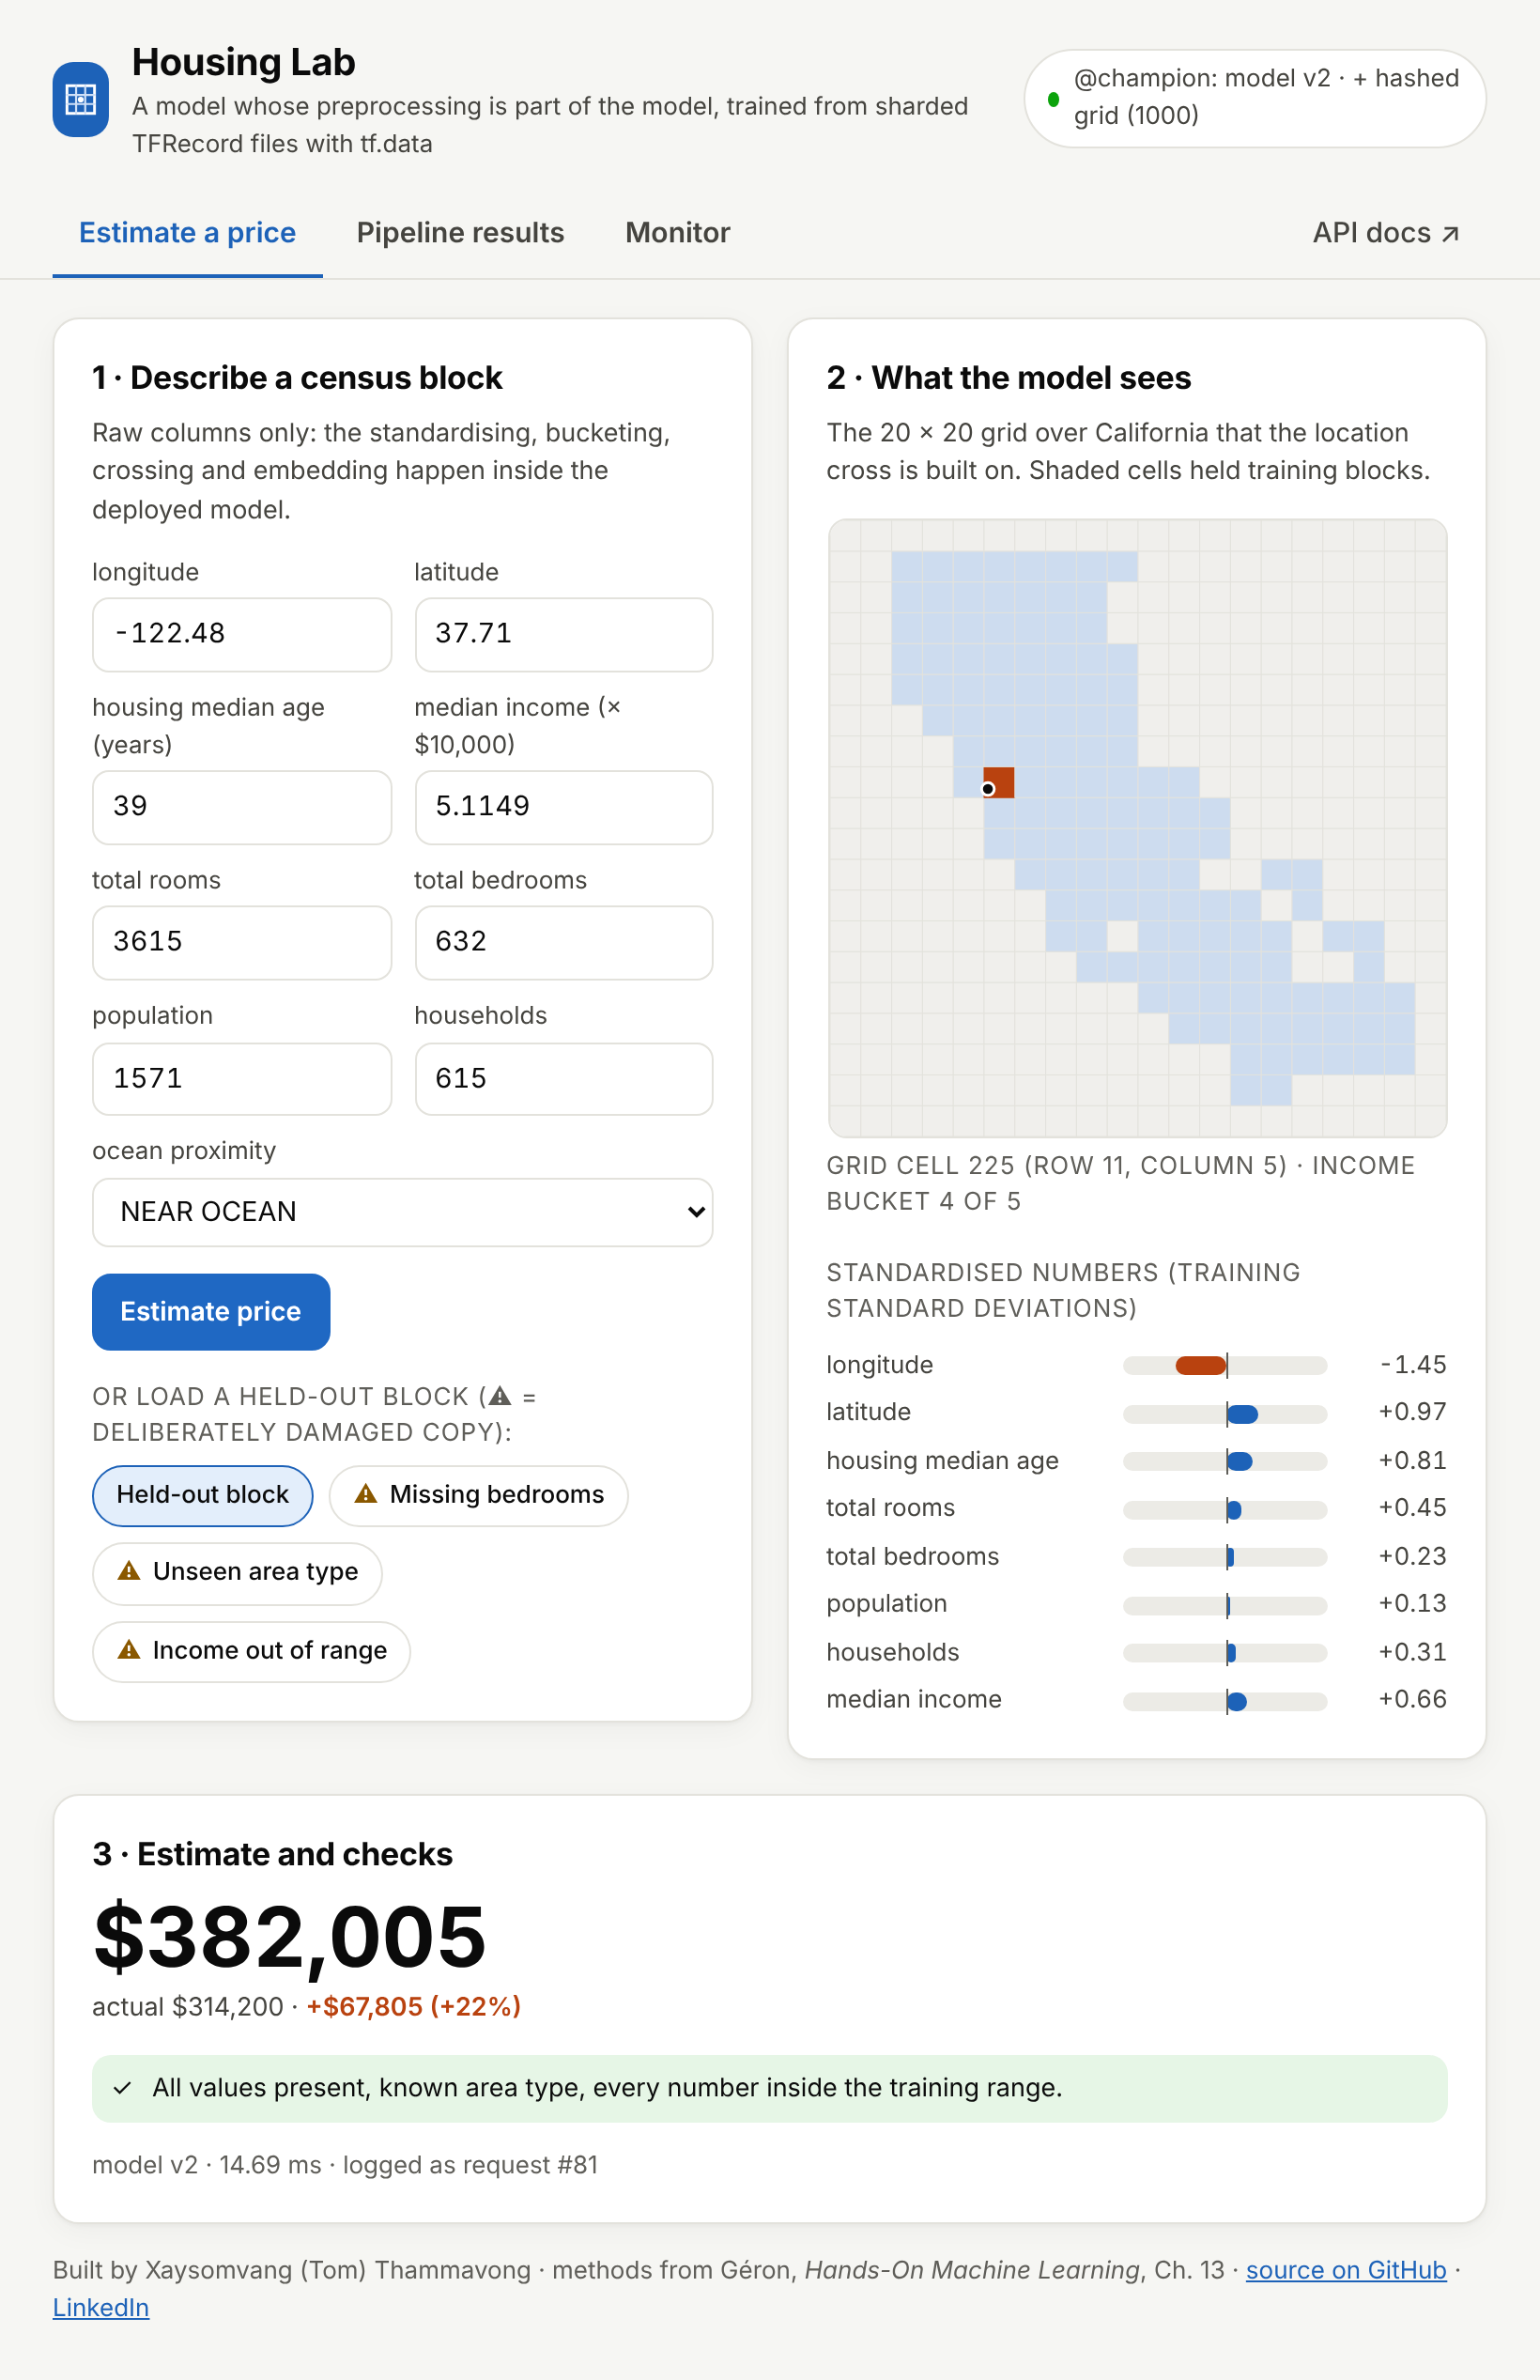
\includegraphics[width=\textwidth,trim=0 145 0 310,clip]{ui_estimate.png}
\caption{The estimate page of the service. Top left: the form with the raw columns of a census block and the buttons that load a held-out block or a deliberately damaged copy of one. Top right: the cell of the location grid and the standardised numbers that the preprocessing layers made of the request. Bottom: the estimate, the actual value of the block, and the data-quality checks.}
\label{fig:ui}
\end{figure}

\FloatBarrier

\section{Mathematical notes}
\label{sec:math}

This section derives the formulas that the experiments use. Most of them are compared with a measurement in the sections above; Sections~\ref{sec:math-embed} and~\ref{sec:math-paired} are definitions and algebra, and the batch diversity is a definition.

\subsection{Prefetching and the time per batch}

Let $t_{\mathrm{in}}$ be the time the input pipeline needs to prepare one batch (read, shuffle, parse, batch) and $t_{\mathrm{s}}$ the time of one training step. Without prefetching the two alternate, so the time for $N$ batches is
\begin{equation}
T_N^{\mathrm{serial}} = N\,(t_{\mathrm{in}} + t_{\mathrm{s}}) .
\end{equation}

With \texttt{prefetch(1)} a background thread prepares batch $k$ while the training step works on batch $k-1$. Write $p_k$ for the time at which batch $k$ is ready and $f_k$ for the time at which step $k$ ends, with $f_0 = 0$. The model assumes that the thread starts preparing batch $k$ as soon as the one-batch buffer is free, that is when step $k-1$ starts (batch 1 starts at time 0, so $p_1 = t_{\mathrm{in}}$), and that every batch takes exactly $t_{\mathrm{in}}$. Step $k$ starts when both the previous step has ended and batch $k$ is ready, so
\begin{equation}
f_k = \max(f_{k-1},\, p_k) + t_{\mathrm{s}} .
\end{equation}

\emph{Case $t_{\mathrm{in}} \le t_{\mathrm{s}}$ (the step is the bottleneck).} Batch $k$ starts to be prepared when step $k-1$ starts, which is at time $f_{k-1} - t_{\mathrm{s}}$, and it is ready at $p_k = f_{k-1} - t_{\mathrm{s}} + t_{\mathrm{in}} \le f_{k-1}$, that is before step $k-1$ ends. Hence $p_k \le f_{k-1}$ for $k \ge 2$, and the maximum is always $f_{k-1}$. Only the first batch has to be waited for: $f_1 = t_{\mathrm{in}} + t_{\mathrm{s}}$ and $f_k = f_{k-1} + t_{\mathrm{s}}$, so
\begin{equation}
f_N = t_{\mathrm{in}} + N\,t_{\mathrm{s}} = t_{\mathrm{in}} + (N-1)\,t_{\mathrm{s}} + t_{\mathrm{s}} .
\end{equation}

\emph{Case $t_{\mathrm{in}} > t_{\mathrm{s}}$ (the input is the bottleneck).} The consumer is faster than the producer, so the buffer is never full and the producer never waits: $p_k = k\,t_{\mathrm{in}}$. Step $k-1$ ends at $f_{k-1} = (k-1)\,t_{\mathrm{in}} + t_{\mathrm{s}} < k\,t_{\mathrm{in}} = p_k$ (this is the induction hypothesis, and it holds for $k=1$ with $f_0 = 0$), so each step starts the moment its batch is ready, $f_k = p_k + t_{\mathrm{s}} = k\,t_{\mathrm{in}} + t_{\mathrm{s}}$, and
\begin{equation}
f_N = t_{\mathrm{in}} + (N-1)\,t_{\mathrm{in}} + t_{\mathrm{s}} .
\end{equation}

Both cases have the form $f_N = t_{\mathrm{in}} + (N-1)\max(t_{\mathrm{in}}, t_{\mathrm{s}}) + t_{\mathrm{s}}$. Dividing by $N$ and letting $N$ grow gives the time per batch
\begin{equation}
\lim_{N\to\infty} \frac{f_N}{N} = \max(t_{\mathrm{in}},\, t_{\mathrm{s}}) ,
\end{equation}
which is the overlap shown in the book's Figure 13-3. This is the dashed line in Figure~\ref{fig:prefetch}, with $t_{\mathrm{in}}$ taken from the measurement with no training step.

\subsection{How well a shuffle buffer mixes sorted data}

A shuffle buffer of size $B$ works as follows: it is first filled with the first $B$ elements of the stream; then, for every output, one of the $B$ elements in the buffer is chosen uniformly at random and sent out, and the next element of the stream takes its place. Suppose the stream is sorted, so the element with input index $i$ has target rank $i$, for $i = 1, \dots, n$.

Consider an element that has just entered the buffer. At each later output it is the chosen one with probability $p = 1/B$, independently of the earlier outputs. The number $G$ of outputs until it leaves therefore has a geometric distribution,
\begin{equation}
\Pr(G = g) = (1-p)^{g-1} p, \qquad
\mathrm{E}[G] = \frac{1}{p} = B, \qquad
\mathrm{Var}(G) = \frac{1-p}{p^{2}} = B(B-1) .
\end{equation}
The buffer holds the first $B$ elements before the first output, and after $m$ outputs it has taken in elements up to $B + m$. Element $i$ can therefore first be chosen at output number $i - B + 1$ (for $i > B$), and it is output at position $(i - B + 1) + (G_i - 1)$, that is
\begin{equation}
O_i = i - B + G_i = i + \varepsilon_i , \qquad \mathrm{E}[\varepsilon_i] = 0, \qquad \mathrm{Var}(\varepsilon_i) = B(B-1) \approx B^{2},
\end{equation}
where the start and the end of the stream, which behave slightly differently, are ignored.

The order correlation reported in the experiments is the Spearman correlation between output position and target. The positions $O_i$ are not exactly ranks, so the Spearman correlation differs slightly from the Pearson correlation of $i$ and $O_i$ that is computed here (by about 0.003 for $B/n = 0.08$ in the experiment); I use the Pearson value as the approximation. Treat $\varepsilon_i$ as independent of $i$. For $i$ uniform on $1,\dots,n$,
\begin{equation}
\mathrm{Var}(i) = \frac{n^{2}-1}{12} \approx \frac{n^{2}}{12} .
\end{equation}
Then $\mathrm{Cov}(i, O_i) = \mathrm{Var}(i)$ and $\mathrm{Var}(O_i) = \mathrm{Var}(i) + B^{2}$, so
\begin{equation}
\begin{aligned}
\rho &= \frac{\mathrm{Cov}(i, O_i)}{\sqrt{\mathrm{Var}(i)\,\mathrm{Var}(O_i)}}
= \frac{\mathrm{Var}(i)}{\sqrt{\mathrm{Var}(i)\,\bigl(\mathrm{Var}(i) + B^{2}\bigr)}} \\
&= \frac{1}{\sqrt{1 + B^{2}/\mathrm{Var}(i)}}
\approx \frac{1}{\sqrt{1 + 12\,(B/n)^{2}}} .
\end{aligned}
\end{equation}

The approximation needs $B$ much smaller than $n$: the noise $\varepsilon_i$ is cut off by the ends of the stream when $B$ is comparable to $n$, and a buffer as large as the data gives a uniformly random order, with $\rho = 0$. The report therefore compares the formula with the measurement only for $B \le n/4$.

\paragraph{Batch diversity.} The second quantity in Figure~\ref{fig:shuffle} is
\begin{equation}
D = \frac{\overline{s}}{s_{\mathrm{all}}}, \qquad
\overline{s} = \frac{1}{K}\sum_{k=1}^{K} \mathrm{sd}(y_{k,1},\dots,y_{k,b}),
\end{equation}
the mean standard deviation of the target inside a batch of $b$ examples, divided by the standard deviation $s_{\mathrm{all}}$ of the whole training set. Batches that look like random draws have $D$ close to 1; consecutive rows of sorted data have $D$ close to 0. Gradient descent works best on the first kind of batch, which is why the book shuffles.

\subsection{Size of a TFRecord file}

The book gives the definition of the \texttt{Example} message and says that a record holds a length, a checksum of the length, the data and a checksum of the data. The byte counts below, the rules of the Protocol Buffers encoding, are not in the book; they are tested by Table~\ref{tab:wire}, where the prediction equals the real size for every record.

A \texttt{tf.train.Example} is a Protocol Buffers message. A length-delimited field with a payload of $L$ bytes occupies
\begin{equation}
F(L) = 1 + v(L) + L \quad\text{bytes},
\end{equation}
where the 1 is the tag (field numbers below 16 need one byte) and $v(L)$ is the number of bytes of $L$ written as a varint: $v(L) = 1$ for $L < 128$, $v(L) = 2$ for $128 \le L < 16384$.

A numeric feature holds a \texttt{float\_list} with one 4-byte float, stored packed. The packed field is $F(4) = 6$ bytes, the \texttt{float\_list} field around it is $F(6) = 8$ bytes, and this is the \emph{Feature} message. A text feature of $s$ bytes is a \texttt{bytes\_list} holding one string, a Feature of $F(F(s))$ bytes. The features are entries of a map from a name to a Feature. An entry with a key of $k$ bytes and a Feature of $f$ bytes has the payload $F(k) + F(f)$, and itself occupies $F\bigl(F(k) + F(f)\bigr)$ bytes in the map. With $E$ the sum of the entry sizes over all features of one row, the serialised row is
\begin{equation}
S = F(E) .
\end{equation}
A missing number is left out of the message, which removes its entry from $E$.

A TFRecord file stores each serialised row as a header (8 bytes for the length and 4 bytes for the CRC of the length), the $S$ bytes of data and a footer (4 bytes for the CRC of the data), so every record carries 16 bytes of framing besides $S$:
\begin{equation}
\text{file size} = \sum_{r=1}^{R} \bigl(S_r + 16\bigr) .
\end{equation}
The experiment computes this sum from the rows without writing a file and compares it with the real file size, byte for byte (Table~\ref{tab:wire}).

\paragraph{A worked example.} The nine numeric names have $9 + 8 + 18 + 11 + 14 + 10 + 10 + 13 + 18 = 111$ bytes in total, and the name \texttt{ocean\_proximity} has 15. A numeric entry has a key of $k$ bytes and a Feature of $f = F(F(4)) = 8$ bytes, so its payload is $F(k) + F(8) = (k + 2) + 10$ and the entry is $F(k + 12) = k + 14$ bytes. The nine numeric entries together have $111 + 9 \cdot 14 = 237$ bytes. The entry of the category, with a string of $s$ bytes, has the payload $F(15) + F(F(F(s))) = 17 + (s + 6)$ and is $F(s + 23) = s + 25$ bytes. With all numbers present $E = 237 + s + 25 = 262 + s$, and because $E \ge 128$ the length of $E$ takes two bytes, so $S = E + 3 = 265 + s$. For \texttt{NEAR OCEAN} ($s = 10$) this gives $S = 275$, the largest size in Table~\ref{tab:wire}. For \texttt{INLAND} ($s = 6$) without \texttt{total\_bedrooms}, whose entry has $14 + 14 = 28$ bytes, $E = 237 - 28 + 31 = 240$ and $S = 243$, the smallest size in the table.

The two CRCs are what detects a flipped byte in the uncompressed file; for the GZIP file the corruption test does not show whether the error came from these checksums or from the decompression.

\subsection{Hashing the location grid into buckets}

The 20 by 20 grid has $n = 400$ cells. The book hashes a crossed feature into $m = 1{,}000$ buckets; it notes that too few buckets cause collisions and that more buckets need a larger embedding table. If the hash behaves like a uniform random function, the number $K$ of cells that land in one given bucket is binomial,
\begin{equation}
K \sim \mathrm{Binomial}\!\left(n, \tfrac{1}{m}\right), \qquad
\Pr(K = k) = \binom{n}{k}\left(\tfrac{1}{m}\right)^{k}\left(1 - \tfrac{1}{m}\right)^{n-k} .
\end{equation}
The expected number of buckets that hold exactly $k$ cells is $m \Pr(K = k)$; this is the second set of bars in Figure~\ref{fig:grid}. A bucket is empty with probability $(1 - 1/m)^{n}$, so the expected number of occupied buckets is
\begin{equation}
\mathrm{E}[\text{occupied}] = m\left[1 - \left(1 - \tfrac{1}{m}\right)^{n}\right] = 1000\,\bigl[1 - 0.999^{400}\bigr] \approx 329.8 ,
\end{equation}
(the number of occupied buckets is a sum of $m$ indicator variables, each equal to 1 with probability $1 - (1-1/m)^n$, and the expectation of a sum is the sum of the expectations), so about $400 - 329.8 = 70.2$ cells are expected to share a bucket with an earlier cell. A given cell shares its bucket with at least one of the other 399 cells with probability $1 - 0.999^{399} \approx 0.33$. In this project the same cells collided in repeated calls of the \texttt{HashedCrossing} layer; I did not check other versions of Keras. What matters for the model is how many \emph{training rows} fall in colliding cells, which the experiment reports because most of the 400 cells hold few rows or none.

\subsection{An embedding is a one-hot vector times a matrix}
\label{sec:math-embed}

Let a categorical feature take values $1, \dots, V$ and let $\mathbf{e}_j \in \{0,1\}^{V}$ be the one-hot vector of value $j$ (a 1 in position $j$, zeros elsewhere). An embedding of dimension $d$ is a matrix $W \in \mathbb{R}^{V \times d}$ whose row $j$ is the learned vector for value $j$. Multiplying the one-hot vector by the matrix selects that row:
\begin{equation}
\mathbf{e}_j^{\top} W = \sum_{i=1}^{V} (\mathbf{e}_j)_i\, W_{i,:} = W_{j,:} .
\end{equation}
So a dense layer without a bias applied to a one-hot input is the same as an embedding lookup, and the lookup is cheaper because it reads one row instead of multiplying $V$ numbers. The gradient of a loss $\mathcal{L}$ with respect to the matrix is
\begin{equation}
\frac{\partial \mathcal{L}}{\partial W} = \mathbf{e}_j \left(\frac{\partial \mathcal{L}}{\partial \mathbf{z}}\right)^{\!\top}, \qquad \mathbf{z} = \mathbf{e}_j^{\top} W ,
\end{equation}
To see this, write $z_l = \sum_k (\mathbf{e}_j)_k W_{k,l}$, so that $\partial z_l / \partial W_{i,m} = (\mathbf{e}_j)_i\,\delta_{l,m}$, and use the chain rule:
\begin{equation}
\frac{\partial \mathcal{L}}{\partial W_{i,m}} = \sum_l \frac{\partial \mathcal{L}}{\partial z_l}\,(\mathbf{e}_j)_i\,\delta_{l,m} = (\mathbf{e}_j)_i\,\frac{\partial \mathcal{L}}{\partial z_m} ,
\end{equation}
the $(i,m)$ entry of $\mathbf{e}_j (\partial \mathcal{L}/\partial \mathbf{z})^{\top}$. It is zero except in row $j$, so a plain gradient-descent step changes only the vector of the value that was seen (the optimiser used in the experiments, Adam, also moves other rows through its running averages). For a batch the gradients of the examples add. A test in the project checks the equality of a dense layer on one-hot input and an embedding layer numerically.

\subsection{Comparing feature sets with paired seeds}
\label{sec:math-paired}

Every feature set is trained with the same $S$ seeds. For a pair of sets $a$ and $b$ and seed $s$, let $r_{a,s}$ and $r_{b,s}$ be the validation RMSE values (the tables of Section~\ref{sec:features} use the validation set for the comparison). Because the same seed fixes the shuffling order and the random numbers that start the training, the errors of the two sets for the same seed are not independent, and the paired differences $d_s = r_{b,s} - r_{a,s}$ remove the part that they share. The mean and the sample standard deviation of the $d_s$ are
\begin{equation}
\bar d = \frac{1}{S}\sum_{s=1}^{S} d_s ,
\qquad
s_d = \sqrt{\frac{1}{S-1}\sum_{s=1}^{S} \bigl(d_s - \bar d\bigr)^2} ,
\end{equation}
and the 95\% confidence interval for the mean difference is the interval of the Student $t$ distribution with $S-1$ degrees of freedom. Chapter 2 of the book applies the same function (\texttt{scipy.stats.t.interval}) to the squared errors of the test instances; here it is applied to the differences between seeds:
\begin{equation}
\bar d \;\pm\; t_{S-1,\,0.975}\,\frac{s_d}{\sqrt{S}} .
\end{equation}
A difference is called clear in the tables when this interval does not contain 0. The interval describes the variation caused by the seeds only. The data split is the same for all runs, so it does not include the variation that another split would add.

\paragraph{The interval of the test RMSE.} Section~\ref{sec:model} uses the function as Chapter~2 does. Let $q_i = (\hat y_i - y_i)^2$ be the squared error of test row $i$, for $i = 1, \dots, n$, with the mean $\bar q$ and the sample standard deviation $s_q$. The mean $\bar q$ is the mean squared error, so $\sqrt{\bar q}$ is the RMSE. Treat the $q_i$ as independent draws with expectation $\mu$, the mean squared error of the model on new rows. The 95\% interval for $\mu$ is $[a, b]$ with
\begin{equation}
a, b = \bar q \;\mp\; t_{n-1,\,0.975}\,\frac{s_q}{\sqrt{n}} .
\end{equation}
The square root is increasing, so $a \le \mu \le b$ holds exactly when $\sqrt{a} \le \sqrt{\mu} \le \sqrt{b}$. The interval $[\sqrt{a}, \sqrt{b}]$ therefore contains $\sqrt{\mu}$ whenever $[a, b]$ contains $\mu$, and it is a 95\% interval for the RMSE:
\begin{equation}
\left[\sqrt{\bar q - t_{n-1,\,0.975}\,s_q/\sqrt{n}}\,,\; \sqrt{\bar q + t_{n-1,\,0.975}\,s_q/\sqrt{n}}\,\right] .
\end{equation}
It is not symmetric about the RMSE, because the square root is not linear. The model is held fixed, so the interval describes only the variation that another sample of $n$ test rows would cause.

\section{Limits and what is not claimed}
\label{sec:limits}

\paragraph{Machine and timings.} All timings come from a cloud machine with two CPU cores and no GPU. Absolute numbers depend on the machine; ratios are what to compare. Each timing is the median of several passes after a warm-up pass, but two measurements of the same configuration still differ: within the run of this report the same CSV pipeline was timed twice and gave \val{noise:a} and \val{noise:b} examples per second (Section~\ref{sec:csv}), \val{noise:pct}\% apart. Differences of that size or less between neighbouring rows of a table are not treated as effects. The tables of only one complete run are stored, so the variation between complete runs is not measured here.

\paragraph{Small data.} The housing data has 20,640 rows and takes about 1.4~MB as a CSV file; the training rows alone take about 0.86~MB. An array in memory is faster than any of the streaming pipelines for such data, and the report shows it. The scale test repeats the training set up to 100 times; this tests how memory and speed of the pipeline grow, and no model is trained on the repeated rows. Even the largest repetition fits in the memory of the machine, so the report shows the different growth of memory but not a case in which pandas fails.

\paragraph{Features.} The book's \texttt{tf.feature\_column} API is replaced by Keras~3 preprocessing layers, so the models are not byte-for-byte the models of the book; in particular I did not check whether \texttt{HashedCrossing} assigns the same buckets as the old crossed column, and the collision counts of Section~\ref{sec:features} are those of the layer used here. The comparison of feature sets uses one split of the data, so its intervals describe the variation caused by the seeds and not the variation another split would cause. The feature sets were not tuned: the sizes of the embeddings other than the book's own (2 dimensions for the categories) and the learning rates were set once.

\paragraph{MNIST.} The version of TFDS used here downloads MNIST from a Google Cloud Storage address. When that address cannot be reached (some firewalls and CI runners cannot reach it, and this project was built in such an environment), the four official files are fetched from a public mirror, checked against the official MD5 checksums and passed to the MNIST builder of TFDS, so that everything after the download is the real \texttt{tfds.load}. The route that this run used is \texttt{\param{D}{source}}. The two inputs that are compared in Part D are trained with the same classifier, but the data from \texttt{tfds.load} are used in the order TFDS delivers them (the book says that the training set it returns is already shuffled), while the TFRecord pipeline shuffles with a buffer of 10,000 images. The comparison of their accuracies is a check that the TFRecord files contain the same data, not a measurement of which input is better.

\paragraph{Choices made after looking at results.} The thresholds of the quality gates are choices of the project, set after looking at the results of a first run; they are meant to catch a broken model, not to define a good one. The feature set of the deployed model is chosen by a rule, the lowest mean validation RMSE of the neural network in Part C. The first version of the configuration named the set \texttt{all features} instead; after the comparison showed that this set was not better than the baseline, the configuration was changed to the rule and the deployment was repeated. The test set played no part in this choice. It is used, however, by the quality gates and by the comparison with the champion, and the thresholds of the gates were set after a first run had been evaluated on it. Chapter~1 of the book warns that a model adapted to a test set by repeated measurements is unlikely to do as well on new data. The test numbers of this report are therefore a final report of this run, not a fresh estimate that no decision has seen.

\paragraph{Sources.} The data loading and preprocessing follow Chapter~13 of the book and the housing data, the split and the confidence interval follow its Chapter~2. The MLOps system around them (Prefect, MLflow, FastAPI, PostgreSQL, Docker Compose, the quality gates, the monitoring and the continuous integration) is not in the book; it follows the structure of the example repository cited in the bibliography.

\subsection{What I learned and what I would do next}

Most of what I learned is about measuring. A step of a pipeline has to be timed with the automatic optimisations of \texttt{tf.data} switched off as well as on, because the optimisations hid most of the effect of the book's steps. One statistic can mislead: reading the files in random order gave an order correlation near 0 while every batch still held almost the same targets. A comparison of two formats needs a control: the TFRecord pipeline differed from the CSV pipeline in the format and in the batching at once. And timings from one machine are compared as ratios, with differences of about \val{noise:pct}\% treated as noise.

The next steps follow from what this report did not separate or did not test:
\begin{itemize}
\item a CSV reader that parses a whole batch of lines in one call, to separate the effect of the TFRecord format from that of batch-wise parsing (Section~\ref{sec:tfrecord});
\item the comparison of \texttt{AUTOTUNE} with the book's fixed values on a machine with more cores and with longer passes, since the cause of the slower \texttt{AUTOTUNE} runs was not investigated (Sections~\ref{sec:csv} and~\ref{sec:tfds});
\item the comparison of feature sets on other splits of the data, so that the intervals include the variation between splits and not only that between seeds (Section~\ref{sec:features});
\item a test of the explanation, so far untested, of why the network gains little from the grid (that its hidden layers build functions of position from raw latitude and longitude), and an experiment that isolates the effect of the hash collisions (Section~\ref{sec:features});
\item data that do not fit in memory, which the scale test, in which every repetition fits comfortably, did not reach (Section~\ref{sec:tfrecord}).
\end{itemize}

\Needspace{14\baselineskip}
\section{Reproducing the results}
\label{sec:repro}

The commands are run from the root of the repository. The quick configuration trains on the same data with fewer repetitions and takes a few minutes. It writes its results to \texttt{reports/quick/}, so the committed results of the full run stay as they are. The full configuration, whose results are in this report, took about 45 minutes on the two-core machine that produced it.

\Needspace{7\baselineskip}
\begin{verbatim}
make install   # Python 3.12 or newer
make test      # offline tests
make quick     # quick configuration; writes reports/quick/
make train     # full experiment; writes the tables, figures and RESULTS.md
make report    # tables of the last run to LaTeX, then this PDF
make up        # the whole stack in Docker (PostgreSQL, MLflow, Prefect, API)
\end{verbatim}

The run that produced this report used the configuration \texttt{configs/full\_flow\_config.yaml} with seed~\runSeed{} on the data with SHA-256 prefix \texttt{\runDataSha}.


\begin{thebibliography}{9}
\bibitem{geron} A.~Géron, \emph{Hands-On Machine Learning with Scikit-Learn, Keras and TensorFlow},
2nd edition, O'Reilly, 2019. Chapter~1 (the use of the test set), Chapter~2 (the housing data,
the split, the confidence interval, the capped values) and
Chapter~13 (the Data API, the TFRecord format, the Features API and TensorFlow Datasets).
\bibitem{example} GitHub user jomariya23156, \emph{full-stack-on-prem-cv-mlops}, public repository,\\
\url{https://github.com/jomariya23156/full-stack-on-prem-cv-mlops}. The structure of the surrounding
MLOps system (one configuration file, train, evaluate and deploy flows, a service that serves the
registered model) follows this project.
\end{thebibliography}

\end{document}
